\documentclass[]{interact}

% ===================== PACKAGES =====================
\usepackage[utf8]{inputenc}
\usepackage[T1]{fontenc}
\usepackage{amsmath,amssymb,amsfonts}
\usepackage{amsthm}
\usepackage{graphicx}
\usepackage{multirow}
\usepackage{booktabs}
\usepackage{array}
\usepackage[hyphens]{url}
\usepackage{algorithm}
\usepackage{algorithmic}
\usepackage{xcolor}
\usepackage[table]{xcolor}
\usepackage{siunitx}
\usepackage{enumitem}
\usepackage{placeins}
\usepackage{float}
\usepackage{pdflscape}
\usepackage{silence}
\usepackage[colorlinks=true,linkcolor=black,citecolor=black,urlcolor=blue]{hyperref}

% Interact-specific citation support updated for Chicago Author-Date
\usepackage[authoryear,round]{natbib}
\renewcommand\bibfont{\fontsize{10}{12}\selectfont}

\usepackage{epstopdf} % To incorporate .eps illustrations
\usepackage[caption=false]{subfig} % Support for small, `sub' figures and tables

% ===================== SETTINGS =====================
\sisetup{detect-weight=true,detect-family=true}
\WarningFilter{latex}{Text page}
\Urlmuskip=0mu plus 2mu

% Custom column type to allow hyphenation in fixed-width columns
\newcolumntype{L}[1]{>{\raggedright\arraybackslash\hspace{0pt}}p{#1}}

\begin{document}

\articletype{RESEARCH ARTICLE}

\title{Explainable Regime Conditioned Mixture of Experts for Financial Anomaly Detection, Risk Capital Calibration, and Cross Market Validation}

\author{
\name{Prashant Hemrajani\textsuperscript{a}, Harshit Kumar\textsuperscript{a}, Sarthak Kumar\textsuperscript{a}, Shashank Shekhar\textsuperscript{a}, Varsha Himthani\textsuperscript{b}, Sayan Mahalik\textsuperscript{a}, and Manoj Kumar Bohra\textsuperscript{a}\thanks{CONTACT Manoj Kumar Bohra. Email: manojkumar.bohra@jaipur.manipal.edu}}
\affil{\textsuperscript{a}Department of IoT and Intelligent Systems, Manipal University Jaipur, Jaipur, Rajasthan, India. Emails: prashant.hemrajani@jaipur.manipal.edu, harshit.23fe10cii00175@muj.manipal.edu, sarthak.23fe10cii00229@muj.manipal.edu, shashank.23fe10cii00220@muj.manipal.edu, sayanmahalik6@gmail.com, manojkumar.bohra@jaipur.manipal.edu; \textsuperscript{b}School of Computer Science Engineering and Technology, Bennett University, Greater Noida, Uttar Pradesh, India. Email: varsha.himthani@gmail.com}
}

\maketitle

\begin{abstract}
Conventional financial anomaly detection relies on static threshold models that ignore volatility regime dynamics. This causes substantial mis-calibration of capital across varied market conditions. To address this, a regime-conditioned mixture of experts (RC-MoE) architecture is proposed. It partitions the market into volatility regimes via realised-volatility quantiles and trains individual experts per regime on eight interpretable features spanning trend, momentum, volatility, market state and tail risk over a 128-day lookback. Experiments are conducted on 2,513 daily observations from the S\&P~500~(US) over 9.7~years (2016--2025) under a leakage-free protocol. Results are further extended to the NASDAQ~(US), Russell~2000~(US), and Bitcoin~(Global). Two key findings emerge. First, unconditional $\text{VaR}_{99}$ fails Kupiec coverage in high-volatility regimes while overcharging capital in stable ones, a result that holds across all four markets. Second, RC-MoE reduces signal frequency by 3.2$\times$ relative to GARCH (6.2\% vs.\ 19.6\% of trading days), improving hedging efficiency by 85\%. The regime-conditioning advantage is independently validated against a global classifier baseline. Factor regression confirms a low market beta (0.63) and near-zero alpha, while Explainability Consistency Index bootstrapping reveals that anomaly drivers shift structurally across regimes. Together, the results establish RC-MoE as a validated framework for regime-conditioned anomaly detection, risk-capital miscalibration correction, and cross-market empirical validation.
\end{abstract}

\begin{keywords}
Financial anomaly detection; mixture of experts; volatility regimes; extreme value theory; Basel III capital calibration; Value-at-Risk; explainability consistency index; S\&P 500
\end{keywords}


\section{Introduction}
Financial markets can be considered complex adaptation systems wherein return distribution is known to display
non-Gaussian behavior, heteroskedasticity, and structure altering regimes~\citep{mandelbrot1963variation, cont2001empirical}. The volatility clustering, fat-tails, and
leverage effect destroy stationarity assumptions inherent in
conventional methods for anomaly detection~\citep{bouchaud2001more, fama1970efficient}. Identification of anomalies within such markets is far from being a
conceptual task, as the occurrence of tail events has caused
severe real failures ranging from Black Monday in 1987 up to
the recent COVID-19 market crash in 2020.

An anomaly in financial markets will always depend
on context. For instance, if volatility is low, a 3\% return per
day would represent an extremely stressful condition; in other
words, under conditions of stress, this very 3\% return could
be absolutely normal. Inability of virtually any existing method to take into account such an anomaly highlights the fact
that there is a problem in detecting the anomaly, in which
magnitude does matter. Parametric techniques that employ
Z-score or control charts operate with thresholds for a non-stationary process, resulting in excessive false alerts or lack
of detection during crisis~\citep{chandola2009anomaly}. Approaches using conditional
volatility such as GARCH~\citep{bollerslev1986a} and EGARCH~\citep{nelson1991egarch} partly resolve
the heteroskedasticity issue, as their initial purpose was volatility estimation~\citep{engle1982arch, hansen1994autoregressive}.

The advent of deep learning techniques has led to an era
of anomaly detectors built around autoencoders, variational autoencoders (VAEs), and transformers with good reconstruction capability within the sample~\citep{darban2023deep, pang2021deep}. Nevertheless, these methods share three major structural issues. First,
the low occurrence rate of tail events (approximately 2\%)
results in serious class imbalance problems. Second, normalization of inputs leads to the loss of information related
to the absolute value of the return, crucial in crash detection~\citep{crepey2022anoma}. Third, black box algorithms provide no justification for the economy behind their decisions, thus violating
Basel III/IV standards~\citep{arrieta2020explainable}. From the empirical side, deep
methods over-fit sample properties and show poor results over
time as structural breaks affect the data generation process~\citep{liu2024times}.

One common feature in all these issues is the lack of regime
structure explicitly introduced in the model. Returns distributions change depending on the volatility regimes~\citep{hamilton1989a, ang2002regime, guidolin2011markov},
yet classical econometrics and deep learning methods alike fail
to include this regime structure in the definition of anomalous
observations. The resulting model suffers from specification
error due to training on unconditional returns distribution;
such model decision boundaries will be too conservative during tranquil times and too liberal in crisis periods.

Our paper begins with a distinct approach: the central challenge of detecting financial anomalies is neither the capacity
of model construction nor its expressiveness, but the proper formulation of the task itself. Rather than creating a more expressive model, we define the problem as a regime-conditioned
structural separability problem. The RC-MoE framework segments financial market behavior into three volatility regimes
via a gating mechanism utilizing rolling realization volatility
quantiles and trains individual expert models for each regime.
Instead of defining anomalies as globally detected outliners,
anomalies are defined as regime-specific tail events where
the threshold of detection depends on the economic condition at hand. In addition, each expert trains separately on a
limited set of economic factors such as trend, momentum,
volatility, tail risk, and liquidity using 128-day rolling windows. The gating function ensures that our segmentation is
economically grounded~\citep{jacobs1991moe, alkilane2024mixma}.

Analysis using 9.7 years of daily S\&P~500 return
data from 2016 to 2025 identifies three practical findings.
First, regime-conditional EVT shows that unconditional
$\text{VaR}_{99}$ violates the Kupiec coverage test in volatile times
($p < 0.001$; actual 2.6\% vs nominal 1.0\%), whereas
Basel~III capital requirements are overestimated by 91\%
in quiet regimes and underestimated by 24\% during
crisis times, exactly when capital adequacy matters the
most. Second, McNemar testing ($\chi^2 = 27.14$, $p < 0.001$)
proves that regime conditioning provides a statistically
distinguishable detection error signature; specifically, the
RC-MoE is a precision detector emitting high-certainty,
rare signals on just 6.2\% of all days compared to 19.6\%
by GARCH, and delivering an average of 85\% more hedging
efficiency for every alert signal (0.315 vs.\ 0.170 pp reduction
in drawdown); the F1 measure gain is not yet significant
in the present data set (paired bootstrap $p = 0.28$); however,
multi-market pooling is a direct solution to this statistical
power challenge. Third, in a regression analysis involving
six Fama-French factors, market beta is reduced to 0.63
($R^2 = 0.69$, $p < 0.001$), with no alpha ($\alpha = -3.74\%$
annually, $p = 0.31$), suggesting the application of the
approach as a portfolio risk-reduction technique; detailed
backtest results for the complete 2016--2025 cycle and
the 2022--2025 bullish period are presented in Section~\ref{sec:multimodel}.

The contributions of this paper are fourfold:

\begin{itemize}
\item We illustrate that VaR models are systematically
under- or over-calibrated depending on volatility regime.
Fitting a generalized Pareto distribution within each
regime, we see that an unconditional $\text{VaR}_{99}$ does not
meet coverage standards in the high-volatility regime
(Kupiec $p < 0.001$; observed 2.6\% vs.\ nominal 1.0\%).
In the internal models approach to Basel~III risk
capital requirements, capital reserves are too large (+91\%
in calm markets) and too small (-24\% in crises) relative
to those from our regime-conditional EVT-VaR model.

\item We present the RC-MoE model, a three-regime
mixture of experts with adaptive multi-detector gates,
trained via a leak-proof regime refit protocol (per-fold regime fitting, rolling expanding window label
generation, circular block bootstrap CIs with $b = 20$
days). McNemar testing for regime effect yields
significance ($\chi^2 = 27.14$, $p < 0.001$); regime conditioning leads to distinct detection performance, although the F1 improvement on our paired test set is
not significant by bootstrapping ($p = 0.28$).

\item The factor exposure profile is assessed using the Fama-French five-factors plus momentum model, with
the market $\beta$ reducing from 1.0 to 0.63 ($R^2 = 0.69$, $p < 0.001$), and alpha being insignificant ($p =
0.31$). The result suggests that the overlay strategy is essentially a risk reduction tool. Each signal generated by the RC-MoE strategy lowers the maximum draw-down by 0.315 pp compared to GARCH(1,1)
with a higher efficiency of around 85\%, and hedges less frequently, only 6.2\% of trading days compared to 19.6\% hedging with GARCH.

\item We develop an index to measure cross-model consistency in explaining the anomaly (Explainability
Consistency Index, ECI), which considers the mean of normalized average pair-wise Kendall's $\tau$ coefficients between the RF, XGBoost, and LightGBM models. Bootstrapping (2{,}000 iterations) reveals
that the drivers of the anomalies depend systematically on regimes, where the ECI increases from
0.646 [0.536, 0.755] in the low-volatility regime to 0.789 [0.702, 0.863] in the high-volatility regime (all regimes' $z$-score $> 3.4$ compared to the random ranking null model; pairwise Wilcoxon rank-sum tests for all pairs $p<0.001$). In addition, we compare GARCH(1,1), Z-score rule, XGBoost, and
LightGBM on S\&P~500 data (2016--2025) under both in-sample and 5-fold temporal protocols.

\end{itemize}
The rest of this paper proceeds in the following manner.
Section~\ref{sec:related} provides a review of related literature along four different research streams. Section~\ref{sec:methodology} outlines the entire RC-MoE
framework, including the process of dataset creation, regime definition, feature engineering, and the mixture-of-expert architecture. Section~\ref{sec:experimental} introduces the leakage-free experimental evaluation process. Section~\ref{sec:ablation} shows results from our ablation study.
Section~\ref{sec:multimodel} shows multimodel classification comparison, economic backtest, hedging efficiency, and conditional VaR analysis for each regime. Section~\ref{sec:explainability} describes explainability analysis, including the metric of ECI.

\section{Related Work}\label{sec:related}
Financial anomaly detection involves four ongoing research
areas: classical statistical methods, deep learning-based time series
models, regime-aware financial models, and interpretable machine
learning~\citep{liu2024times, chandola2009anomaly}. However, unlike generic anomaly detection, financial data have heteroskedasticity, regime changes, extremely imbalanced classes, and structural breaks. All four streams will be
described in turn.

\subsection{Statistical/Econometric Methods}

Initial attempts at anomaly detection based on parametric
models that assumed stationary distribution of returns~\citep{mandelbrot1963variation, cont2001empirical, fama1970efficient}.
The Z-score, control charts, and standard deviation rule mark the
anomaly as deviation from a fixed reference distribution. While
computationally fast, these methods cannot address issues of non
stationarity or volatility clustering and hence provide excessive false
positives during calm times and fail to detect real anomalies in a
crisis situation~\citep{engle1982arch, bollerslev1986a}.

Conditional volatility models such as GARCH~\citep{bollerslev1986a}, EGARCH~\citep{nelson1991egarch}
and stochastic volatility models use variance which is time varying
and detect anomaly relative to the conditional distribution. However, these models were developed for volatility forecasting and risk
management purposes and thus are evaluated by different criteria than precision and recall.

\subsection{Regime-Aware Models and Mixture-of-Experts Architecture}

The concept of financial market regimes is widely used in literature
for addressing topics such as the volatility clustering phenomenon and
the business cycle effect. Models based on switching regimes, such
as the Markov Switching Models~\citep{hamilton1989a} and Hidden Markov Models,
have usually been used for identifying hidden regimes, such as bull
market regime, bear market regime, and crisis regimes~\citep{ang2002regime, guidolin2011markov}.
While simpler and deterministic techniques have been devised that use
realized volatility quantiles or variance cutoffs, in most of the existing
researches, the market regime information has not been employed in
either refining the anomaly concept or for the evaluation phase.

Current MoE architectures in finance belong to one of two categories:
forecasting-related Mixture of Experts (MoE) models~\citep{alkilane2024mixma}
where the inputs go to expert predictors, but return/price prediction is the main objective.
None offers regulatory validation. The work which is most similar to ours is
Li and Fan~\citep{fan2025expla}, where an adaptive MoE model employing a GNN-based
gating network has been used for deviation detection from local equity.
It employs four experts, whose choice is arbitrary, operates on short-term OOS
test sets without leakage-proof time-series protocol, and lacks EVT/capital adequacy analysis. The present work takes a structurally different path: regimes are defined on an observable economic variable (realized volatility), anomalies are redefined conditionally on the current regime rather than against a global distribution, and formal regulatory validation via Kupiec backtests and Basel~III capital adequacy analysis is provided as a primary contribution.

\subsection{Deep Learning for Anomaly Detection}

Anomaly detection using deep learning algorithms has progressed due to developments in representation learning~\citep{darban2023deep, pang2021deep}. Recurrent networks, convolutional networks, variational autoencoders, and transformers exhibit high in-sample performance on financial time-series data~\citep{su2025anoma, wu2024anoma, cao2024autom}. Three structural issues prevent them from being used effectively in financial applications. First, rare tail observations (about 2\%) cause very severe class imbalance. Second, normalization of inputs prevents them from detecting the actual magnitude of returns that is critical for crash detection. Third, deep learning algorithms typically learn noise rather than economic structure, especially in small samples. The development of attention mechanisms, ensembles, and focal loss has led to improvements in in-sample performance but failed to solve the interpretability problem, which is a hard constraint under Basel~III/IV~\citep{arrieta2020explainable}. Long-term forecast performance is poor because regimes shift invalidating in-sample patterns~\citep{liu2024times}.

\subsection{Interpretable Machine Learning in Finance}
\label{subsec:rel_interpretable}

Interpretability is mandatory by regulation in finance, not just a
preference~\citep{arrieta2020explainable}. Linear factor models, decision trees, and
shallow ensemble approaches~\citep{breiman2001random, friedman2001greedy} are still in use because
they generate interpretable decision rules, even though other,
more flexible, neural networks can be applied. Financial theories
are successfully utilized to construct highly predictive input representations through factor-based representations. Instance-wise post-hoc explanations by means of the SHAP~\citep{lundberg2017shap}
and LIME~\citep{ribeiro2016lime} methods are gaining ground in finance~\citep{wang2024adapt},
but the instability of the latter for rare events renders aggregative explanations by factor and regime much more desirable.

Our approach tackles the issue on two levels: factor-based
input representation ensures economic consistency in the input
representation level, and shallow ensemble expert models provide transparent and auditable decision rules in the model
level. Besides instance-level explanation, we propose the
Explainability Consistency Index (ECI) that formalizes cross-model
feature importance agreement among the expert families as well as across the volatility regimes, a regime-disaggregated
consistency measurement that has not been addressed yet.

\begin{table}[p]
\tbl{Literature review: financial anomaly detection methods (2008--2025)}
{\scriptsize
\renewcommand{\arraystretch}{1.2}
\setlength{\tabcolsep}{3pt}
\resizebox{\textwidth}{!}{%
\begin{tabular}{>{\raggedright\arraybackslash\hspace{0pt}}p{2.2cm} >{\raggedright\arraybackslash\hspace{0pt}}p{0.7cm} >{\raggedright\arraybackslash\hspace{0pt}}p{2.5cm} >{\raggedright\arraybackslash\hspace{0pt}}p{1.8cm} >{\raggedright\arraybackslash\hspace{0pt}}p{2.0cm} >{\raggedright\arraybackslash\hspace{0pt}}p{2.0cm} >{\raggedright\arraybackslash\hspace{0pt}}p{1.2cm} >{\raggedright\arraybackslash\hspace{0pt}}p{0.6cm} >{\raggedright\arraybackslash\hspace{0pt}}p{7.5cm}}
\toprule
\textbf{Author(s)} & \textbf{Year} & \textbf{Method} & \textbf{Dataset} & \textbf{Anomaly Target} & \textbf{Eval Paradigm} & \textbf{Regime Aware} & \textbf{XAI} & \textbf{Key Limitation} \\
\midrule
Liu et al.\ \citep{liu2008isolation} & 2008 & Isolation Forest & Syn./ HTTP & Global Outlier & In-sample Fit & No & No & No temporal structure; global threshold \\
Hamilton \citep{hamilton1989a} & 1989 & Markov-Switching & US GNP & Latent State Shift & In-Sample Fit & Yes & No & Two regimes only; constant transitions \\
Chandola et al.\ \citep{chandola2009anomaly} & 2009 & Survey Methods & Multiple & Academic Domain & Literature Review & No & No & No finance-specific evaluation \\
Cont \citep{cont2001empirical} & 2001 & Stylized Facts & Glob.\ Equities & Empirical Fact & Descriptive Stats & No & N/A & Descriptive; no detection framework \\
Cr\'{e}pey et al.\ \citep{crepey2022anoma} & 2022 & PCA + Neural Net & Syn.\ Finance & Global Deviation & Short-Horizon OOS & No & Low & Relies on synthetic data; supervised \\
Song \citep{song2023anoma} & 2023 & VAE-Transformer & DeFi & Recon\-struction & Short-Horizon OOS & No & Low & Single DeFi dataset; no regime analysis \\
Darban et al.\ \citep{darban2023deep} & 2024 & Survey: Deep TSAD & Multi-domain & Academic Domain & Literature Review & No & No & No standardized evaluation protocol \\
Wang \citep{wang2024adapt} & 2024 & SHAP + Ensemble & CIS Fraud & Global Deviation & Single-Period OOS & No & High & No regime conditioning; fraud-specific \\
Cao \& Guo \citep{cao2024autom} & 2024 & RL-based selection & SWaT/ COBT & Recon\-struction & Short-Horizon OOS & No & Low & Threshold-dependent; no financial regimes \\
Li \& Fan \citep{fan2025expla} & 2025 & Adaptive MoE + GNN & US equities & Local Deviation & Short-Horizon OOS & Yes & High & Fixed four-expert taxonomy; no VaR analysis \\
Bakumenko \citep{bakumenko2025advan} & 2025 & LLM Embeddings & Gen.\ Ledger & Semantic Outlier & Short-Horizon OOS & No & Low & Limited to accounting data \\
Su \citep{su2025anoma} & 2025 & WV+LSTM+\newline Transformer & S\&P/ Binance & Recon\-struction & Short-Horizon OOS & No & No & Static anomaly thresholds \\
Zhou et al.\ \citep{zhou2025kanad} & 2025 & KAN-AD (Fourier) & KPI/ SMAP & Recon\-struction & Short-Horizon OOS & No & Low & Univariate focus; no financial regimes \\
Alkilane et al.\ \citep{alkilane2024mixma} & 2024 & MixMamba MoE & ETT/ Weather & Point Prediction & Short-Horizon OOS & Yes & No & Forecasting only; no anomaly detection \\
Luo \citep{luo2025robus} & 2025 & Causal Hypergraph & Yelp/ Amazon & Global Outlier & Cross-Sectional & No & Med & Complex; fraud-specific; not time-series \\
Pang et al.\ \citep{pang2021deep} & 2021 & Survey: Deep AD & Multi-domain & Academic Domain & Literature Review & No & No & No standardized financial evaluation; regime shifts ignored \\
Breiman \citep{breiman2001random} & 2001 & Random Forest & UCI / Finance & Global Outlier & Cross-Val OOB & No & Med & Static global threshold; no temporal or regime structure \\
Sch\"{o}lkopf et al.\ \citep{scholkopf2001estimating} & 2001 & One-Class SVM & UCI/ Synthetic & Density Support & In-Sample CV & No & Low & Kernel choice sensitive; quadratic training cost; no temporal dynamics \\
Engle \& Manganelli \citep{engle2004caviar} & 2004 & CAViaR Reg.\ Quantile & US/UK Equities & VaR Tail & Rolling OOS & Implicit & Low & Predicts conditional quantile only; no binary anomaly classification \\
Wu et al.\ \citep{wu2024anoma} & 2024 & RNN + Latent VAR & Financial TS & Recon\-struction & Short-Horizon OOS & No & No & Black-box; requires supervised labels; no regime conditioning \\
\bottomrule
\end{tabular}%
}}
\label{tab:lit_review}
\end{table}

\begin{table}[htbp]
\tbl{Taxonomy of Financial Anomaly Detection Objectives}
{\small
\renewcommand{\arraystretch}{1.15}
\begin{tabular}{L{0.26\textwidth} L{0.32\textwidth} L{0.34\textwidth}}
\toprule
\textbf{Dimension} & \textbf{Predictive Paradigm} & \textbf{Structural (This Work)} \\
\midrule
Anomaly Definition & Global deviation & Regime-conditional tail \\
Primary Objective & Forecast accuracy & Structural separability \\
Evaluation Focus & OOS performance & In-sample regime isolation \\
Model Preference & High-capacity DL & Interpretable factors \\
Deployment Goal & Real-time prediction & Diagnostic analysis \\
\bottomrule
\end{tabular}}
\label{tab:taxonomy}
\end{table}

\subsection{Positioning of This Work}

Table~\ref{tab:lit_review} presents a structured review of some representative past research in all the four paradigms. Table~\ref{tab:taxonomy} illustrates the conceptual distinction between the predictive and structural paradigm for the detection of financial anomalous observations. The current research study differs from past literature in the following important aspects. First, it applies an approach of detecting anomalies in the context of regime conditional structural separability, as opposed to global prediction paradigm. Secondly, this paper integrates knowledge about regimes in both the definition of anomalies and in the architecture of the model through the use of adaptive mixture of experts (MoE) gating network.

Thirdly, the current study involves a long-run longitudinal analysis, differentiating between in sample structural separability and out-of-sample prediction, which is rarely done in recent literature. Table~\ref{tab:comparison} captures the approach followed in this study relative to major paradigms.

\begin{table*}[t]
\tbl{Comparison of Anomaly Detection Frameworks in Finance}
{\resizebox{\textwidth}{!}{%
\begin{tabular}{lcccc}
\toprule
\textbf{Framework} & \textbf{Core Methodology} & \textbf{Regime Awareness} & \textbf{Interpretability} & \textbf{Primary Objective} \\
\midrule
Statistical (Z-Score) & Global Thresholding & None & High & Pointwise Detection \\
GARCH/Vol Models & Conditional Variance & Implicit & Medium & Volatility Forecasting \\
Deep Learning (VAE/LSTM) & Reconstruction Error & None & Low & Signal Reconstruction \\
\textbf{Proposed (Regime MoE)} & \textbf{Conditioned Structural Separability} & \textbf{Explicit} & \textbf{High} & \textbf{Regime-Specific Diagnosis} \\
\bottomrule
\end{tabular}%
}}
\label{tab:comparison}
\end{table*}

Past techniques can be distinguished along four dimensions. For instance, most techniques define anomalies based on unconditional distributions while regime-conditional techniques acknowledge that the same amount of returns can be normal in crisis regimes and abnormal in calm regimes. On the third dimension, high capacity deep learning models sacrifice interpretability for expressive power, while factor and tree models maintain economic interpretability. Lastly, on the fourth dimension, most existing studies are performed under the assumption of stationarity or short horizon, and very few long horizon analyses take into consideration regime change.

Unlike existing studies, our research is unique in all four dimensions because it introduces regime-conditional anomalies, favors structure extraction over prediction precision, makes use of economically interpretable factor models, and evaluates results over a span of nine years.

\subsection{Research Gap}
Despite the diversity of the earlier studies, an important limitation remains.
No existing method jointly (a) defines financial anomalies using the current
volatility regime rather than a universal return distribution; (b) assesses
such a conditional definition using rigorous regulatory risk measures through
EVT-based VaR backtesting and Basel~III capital requirements; and (c) explains
anomalies conditional on the current regime using a statistical model that
formally quantifies the consistency of regime-specific explanations. Among
concurrent studies, Li and Fan~\citep{fan2025expla} utilize an adaptive MoE
approach for equity-return prediction with a fixed taxonomy of four experts,
while neither conditioning anomaly definitions on regimes nor performing
capital miscalibration assessment under leakage-free protocols.

% ===================== METHODOLOGY =====================
\section{Methodology}
\label{sec:methodology}
This subsection gives a description of the proposed RC-MoE framework. The framework has three modules: (i) a factor decomposition process which decomposes each rolling return window into eight economic factors (trends, momentum, volatility, hidden regime, and tail risks); (ii) a gated model with adaptive voting that fuses outputs of the three independent volatility detectors (rolling quantile, Gaussian HMM, and static quantile) with confidence weighting; and (iii) a regime-dependent meta-model, which assigns the factor vectors to appropriate experts based on the regime condition. In each rolling window, the framework conducts factor analysis, gating, and regime-dependent expert scoring to calculate the anomaly score. By training regime-specific expert ensembles, the anomaly structure is not mixed between calm and crisis regimes~\citep{hamilton1989a}.

The subsections below cover data and evaluation setup, regime definition, factor engineering, and the mixture-of-experts architecture.

\subsection{Dataset Description}
The RC-MoE method is tested using the S\&P~500 Index (\^{}GSPC),
which is the most prominent large cap index in the United States.
The data includes daily open, high, low, close, and volume values from
2015--2025. This index is selected because of its history going through
multiple market regimes as well as the presence of regime-defining events
that include the 2015--2016 oil shock, 2018 volatility shock, 2020 COVID
crash, and 2022 inflation-induced market drawdown~\citep{cont2001empirical}. The data was split
into overlapping windows of 128 days (rolling, stride 1) without shuffling. Since the 128
days window and 252 days rolling quantile-based regimes estimation use the
first year of data, the period considered for evaluation spans 2016--2025. The
anomalies were defined based on thresholds calculated from regime-conditional
return distribution at the 98th percentile. Thresholds at point $t$ include only
historical information $\{|r_0|, \ldots, |r_{t-1}|\}$ via a rolling expanding quantile (minimum
observations of 20), so there is no forward-looking information used when
defining the label. The anomaly frequency is approximately 2.0\%. The regimes
were defined as low, medium, or high based on rolling quantiles of volatility,
as detailed in Section~\ref{sec:regime_definition}.

Three unique thresholds will be encountered throughout this
paper, based on the careful consideration of a difference in
evaluation granularity and threshold selection, not an ambiguity in
terminology. (i) For the RC-MoE model presented here, the
window based framework uses a 98th percentile threshold,
based on 128-day windows, generating approximately 2.0\%
anomalous windows. (ii) In Section~\ref{sec:multimodel}, the daily anomaly rate in
the comparison between models is obtained from a 95th percentile
threshold applied directly to the raw return series, resulting in
approximately 3.1\% (approximately 76 anomalies among 2{,}455 daily
returns). (iii) Table~\ref{tab:datasets} provides 95th percentile anomaly counts on
128-day windows in four markets (4.7--6.8\%), the percentage being
higher due to shorter window-count denominator than the raw day
count. Downstream evaluations specify which criterion is employed.

Three data integrity practices are followed: labels and features are
based only on backward-looking data; returns are not globally
normalized, allowing the retention of tail magnitudes necessary for
crash detection; imbalanced classes are accounted for using cost-sensitive learning, without synthetic sample expansion. Pre-processing
techniques such as SMOTE and global normalization discard precisely
the magnitudes necessary for detecting extreme events~\citep{bouchaud2001more}.

The dataset displays different distribution characteristics at
different volatility regimes.

\subsection{Leakage-Free Evaluation Protocol}
\label{sec:leakage_free}
We identified and closed six sources of look-ahead bias. Per-fold normalization: StandardScaler is fitted exclusively on each training partition and applied to the held-out test partition, replacing global Z-score normalization that would otherwise import test-set statistics. Per-fold regime classification: all three regime detectors (rolling quantile detector, Gaussian Hidden Markov Model, and static quantile detector) are recalibrated for each training partition and assign regimes to the test partition using only the final state probabilities of the training partition. Rolling expanding window anomaly labels: the threshold for labeling anomalies is calculated only based on $\{|r_0|, \ldots, |r_{t-1}|\}$ by way of expanding quantiles (with a minimum sample size of 20) so as to eliminate the circularity associated with using quantiles across the entire dataset to calculate labels. Training-only probability threshold optimization: Decision thresholds are selected solely from the probabilities outputted on the training folds, without ever using information from the test labels in the selection process. Circular block bootstrap confidence intervals: Confidence intervals are calculated with blocks of size $b = 20$ trading days in order to preserve autocorrelation of financial time series, rather than the independent identically distributed bootstrap, which yields artificially tight intervals in the case of autocorrelation.

\subsection{Problem Formulation}
\label{sec:problem_formulation}
The task of detecting financial anomalies is modeled as
the regime-dependent separability problem as opposed to forecasting and trading problems. The goal of this task is not to
forecast future anomalies but rather to identify if there exist
stable structural signatures which are unique and discriminative to anomalies within the specific regime of volatility. As
such, the economic backtest performed in this paper is a consequence of detecting such economic value, not the intended
trading strategy as described below.

Let $\{P_t\}_{t=1}^{T}$ denote the daily closing prices of a financial asset. Log returns are defined as $r_t = \log(P_t / P_{t-1})$. Rather than modeling pointwise returns, the series is segmented into overlapping rolling windows~\eqref{eq:window}
\begin{equation}
    W_t = \{ r_{t-L+1}, \ldots, r_t \}, \quad L = 128,
    \label{eq:window}
\end{equation}

where each sliding window constitutes a local regime in the
market capturing medium- to long-term behavior characterized by volatility clustering, momentum decay, and tail risk
accumulation~\citep{bouchaud2001more}. Both the features and labels used for training were computed based on the backward-looking data only,
thus eliminating any potential for look-ahead bias. Nevertheless, the distributional properties of the sliding windows differ significantly depending on the regime of volatility, thus requiring that the anomaly threshold be regime-dependent.

\subsection{Regime-Conditioned Market States and Anomaly Definition}
\label{sec:regime_definition}
However, financial markets exhibit heteroskedasticity and non-stationarity~\citep{bouchaud2001more, hamilton1989a},
which suggests that a universal probability distribution for describing the behavior of
financial markets is not enough for all cases. In our approach, a particular volatility
regime is associated with each window $W_t$. The key ingredient of the regime detection
scheme is the realized volatility $\sigma_t$, defined as the sample standard deviation of log
returns over window $W_t$:

\begin{equation}
\sigma_t =
\sqrt{
\frac{1}{L - 1}
\sum_{i=1}^{L}
(r_{t-i+1} - \bar{r}_t)^2
}
\label{eq:volatility}
\end{equation}

where $\bar{r}_t$ is the mean return in window $W_t$. Our scheme does not rely on a quantile
rule but uses an adaptive gating method that integrates three regime detectors running
in parallel.

Detector 1 (Rolling Quantile): The adaptive 252-day rolling
quantile detector divides $\sigma_t$ into three regimes~\eqref{eq:regime} according to
tercile quantiles estimated based on trailing volatility measurements over the last year:

\begin{equation}
R_t^{\text{roll}} =
\begin{cases}
0, & \text{if } \sigma_t \le Q_{33}(\Sigma_{t-252:t}), \\
1, & \text{if } Q_{33}(\Sigma_{t-252:t}) < \sigma_t \le Q_{66}(\Sigma_{t-252:t}), \\
2, & \text{if } \sigma_t > Q_{66}(\Sigma_{t-252:t}),
\end{cases}
\label{eq:regime}
\end{equation}

where $\Sigma_{t-252:t}$ denotes the trailing set of volatility estimates.
A rolling window makes the regime thresholds dynamic in
order to reflect the changing nature of financial markets.

Detector 2 (Gaussian HMM): This detector employs a three
state Gaussian Hidden Markov Model (HMM) to determine
latent states of volatility according to the Baum--Welch algorithm~\citep{hamilton1989a}. Transition probabilities and a regime persistence
factor are modeled within the HMM, and state probabilities
are calculated for each regime $k \in \{0,1,2\}$:
\begin{equation}
P(R_t^{\text{HMM}} = k \mid \sigma_{1:t})
\label{eq:hmm_prob}
\end{equation}

This detector supplies probabilities instead of deterministic
regime classifications. As per the leakage-free evaluation
protocol (Section~\ref{sec:leakage_free}), the entire set of three detectors is
re-calibrated at each training fold. Test-fold regime labels are
predicted based on projected thresholds without observing
future volatilities.

Detector 3 (Static Quantile): The baseline detector uses
quantile-based regimes estimated solely from the training-fold
data available prior to the current fold boundary. This forms a
stable point of reference used to anchor the other adaptive detectors.
In the absence-of-leakage regime detection algorithm presented in
Section~\ref{sec:leakage_free}, this estimator is only applied to the respective
training set partitions and not influenced by any volatility observations
beyond the regime assignment period.

The resulting regime assignment of each of the three detectors
$D_i$ is complemented with a confidence value $C_t^{(i)} \in [0,1]$,
and the final fused regime assignment is chosen by weighted
voting according to:

\begin{equation}
\begin{split}
\hat{R}_t &= \arg\max_{k \in \{0,1,2\}} \\
&\quad \sum_{i=1}^{3} C_t^{(i)} \cdot \mathbb{I}(R_t^{(i)} = k),
\end{split}
\label{eq:fusion}
\end{equation}

The confidence in the decision is defined as
$C_t = \max_k P(\hat{R}_t = k)$, where $P(\hat{R}_t = k)$ denotes the
normalized weighted vote count for regime $k$. Multi-detector
fusion allows for robustness to failures of a particular detector: the
rolling quantile adjusts to the local situation, HMM considers
regime persistence, while the static quantile prevents excessive drift.

The fused confidence $C_t$ will then dictate the routing policy.
If $C_t \geq \tau_c$, ($\tau_c = 0.6$), a hard routing will route the observation
solely to expert $E_{\hat{R}_t}$. On the other hand, when $C_t < \tau_c$,
meaning that regime classification is ambiguous close to boundaries,
the soft routing will allocate the observation to regimes' adjacent experts
depending on their probabilities.

\begin{equation}
w_t^{(k)} =
\begin{cases}
\mathbb{I}(k = \hat{R}_t), & \text{if } C_t \geq \tau_c \text{ (hard)}, \\
P(\hat{R}_t = k), & \text{if } C_t < \tau_c \text{ (soft)}.
\end{cases}
\label{eq:routing}
\end{equation}

This intelligent strategy solves one problem inherent in the hard
gating mechanism where observations close to regime boundaries
contribute information to more than one expert, reducing possibility
of misclassification in cases of regime switching. The theoretical
rationale for using volatility gates on raw returns auto-correlation
will drop very fast to zero, making returns unpredictable in direction;
however, the squared return auto-correlation is a long memory
process, which means there exists clustered volatility, which could
be investigated using backward looking observation~\citep{cont2001empirical}. Each regime
possesses around 33\% of observations, although returns distribution
differs greatly between regimes.

Anomalies thresholds are computed conditionally on
the current regime, which means that the same return values
may mean different things depending on the regime.
For any given regime $r \in \{0,1,2\}$, the threshold~\eqref{eq:threshold}
is defined as the $(1-\alpha)$-quantile of the distribution of the
conditional absolute returns:

\begin{equation}
\tau_r = Q_{1-\alpha}(|r| \mid R_t = r), \quad \alpha = 0.02,
\label{eq:threshold}
\end{equation}

and the anomaly indicator is determined by~\eqref{eq:anomaly}:

\begin{equation}
A_t = \mathbb{I}(|r_t| > \tau_{R_t}).
\label{eq:anomaly}
\end{equation}

This approach takes into account economically relevant distinctions
between ordinary market fluctuations and truly extreme stress
events, as is typical for returns that are heavy tailed and volatility
clustered~\citep{bouchaud2001more}.

Regarding the separation objective, the task is clear:
for any given regime $r$, one needs to determine the function
$f_r : \mathbb{R}^d \rightarrow [0,1]$ such that
$f_r(F_t^{\text{anomaly}}) > f_r(F_t^{\text{normal}})$.

As tools for assessing separability, Precision, Recall, and F1-score offer diagnostic value but not assurance of generalizability. The use of such measures does not imply that decision boundaries remain constant over decades, in that results are considered to be upper limits of discrimination within the context of certain fixed definitions of regimes. Thresholds that rely on regimes ensure a constant rate of anomaly occurrence regardless of the market environment, but not so with raw returns – see the following subsection.

\subsection{Factor-Based Representation}
\label{sec:factors}
Raw return sequences exhibit large dimensionality, strong autocorrelation, and noise dominance, making sequence modeling highly inefficient and potentially biased toward memorization. On the other hand, each window $W_t \in \mathbb{R}^{L \times F}$ (with $L = 128$, and $F$ is the number of raw inputs) is transformed into the low-dimensional and interpretable factor vector $F_t = \phi(W_t) \in \mathbb{R}^d$, where $d \ll L \times F$. Such transformations increase the SNR and preserve the absolute scale of the returns, which is usually downweighted in normalization-based approaches, but plays an important role in detecting extreme financial events~\citep{bouchaud2001more}. Figure~\ref{fig:phase1_pipeline} provides an overview of the entire pipeline of factor generation process.

\begin{figure*}[!t]
\centering
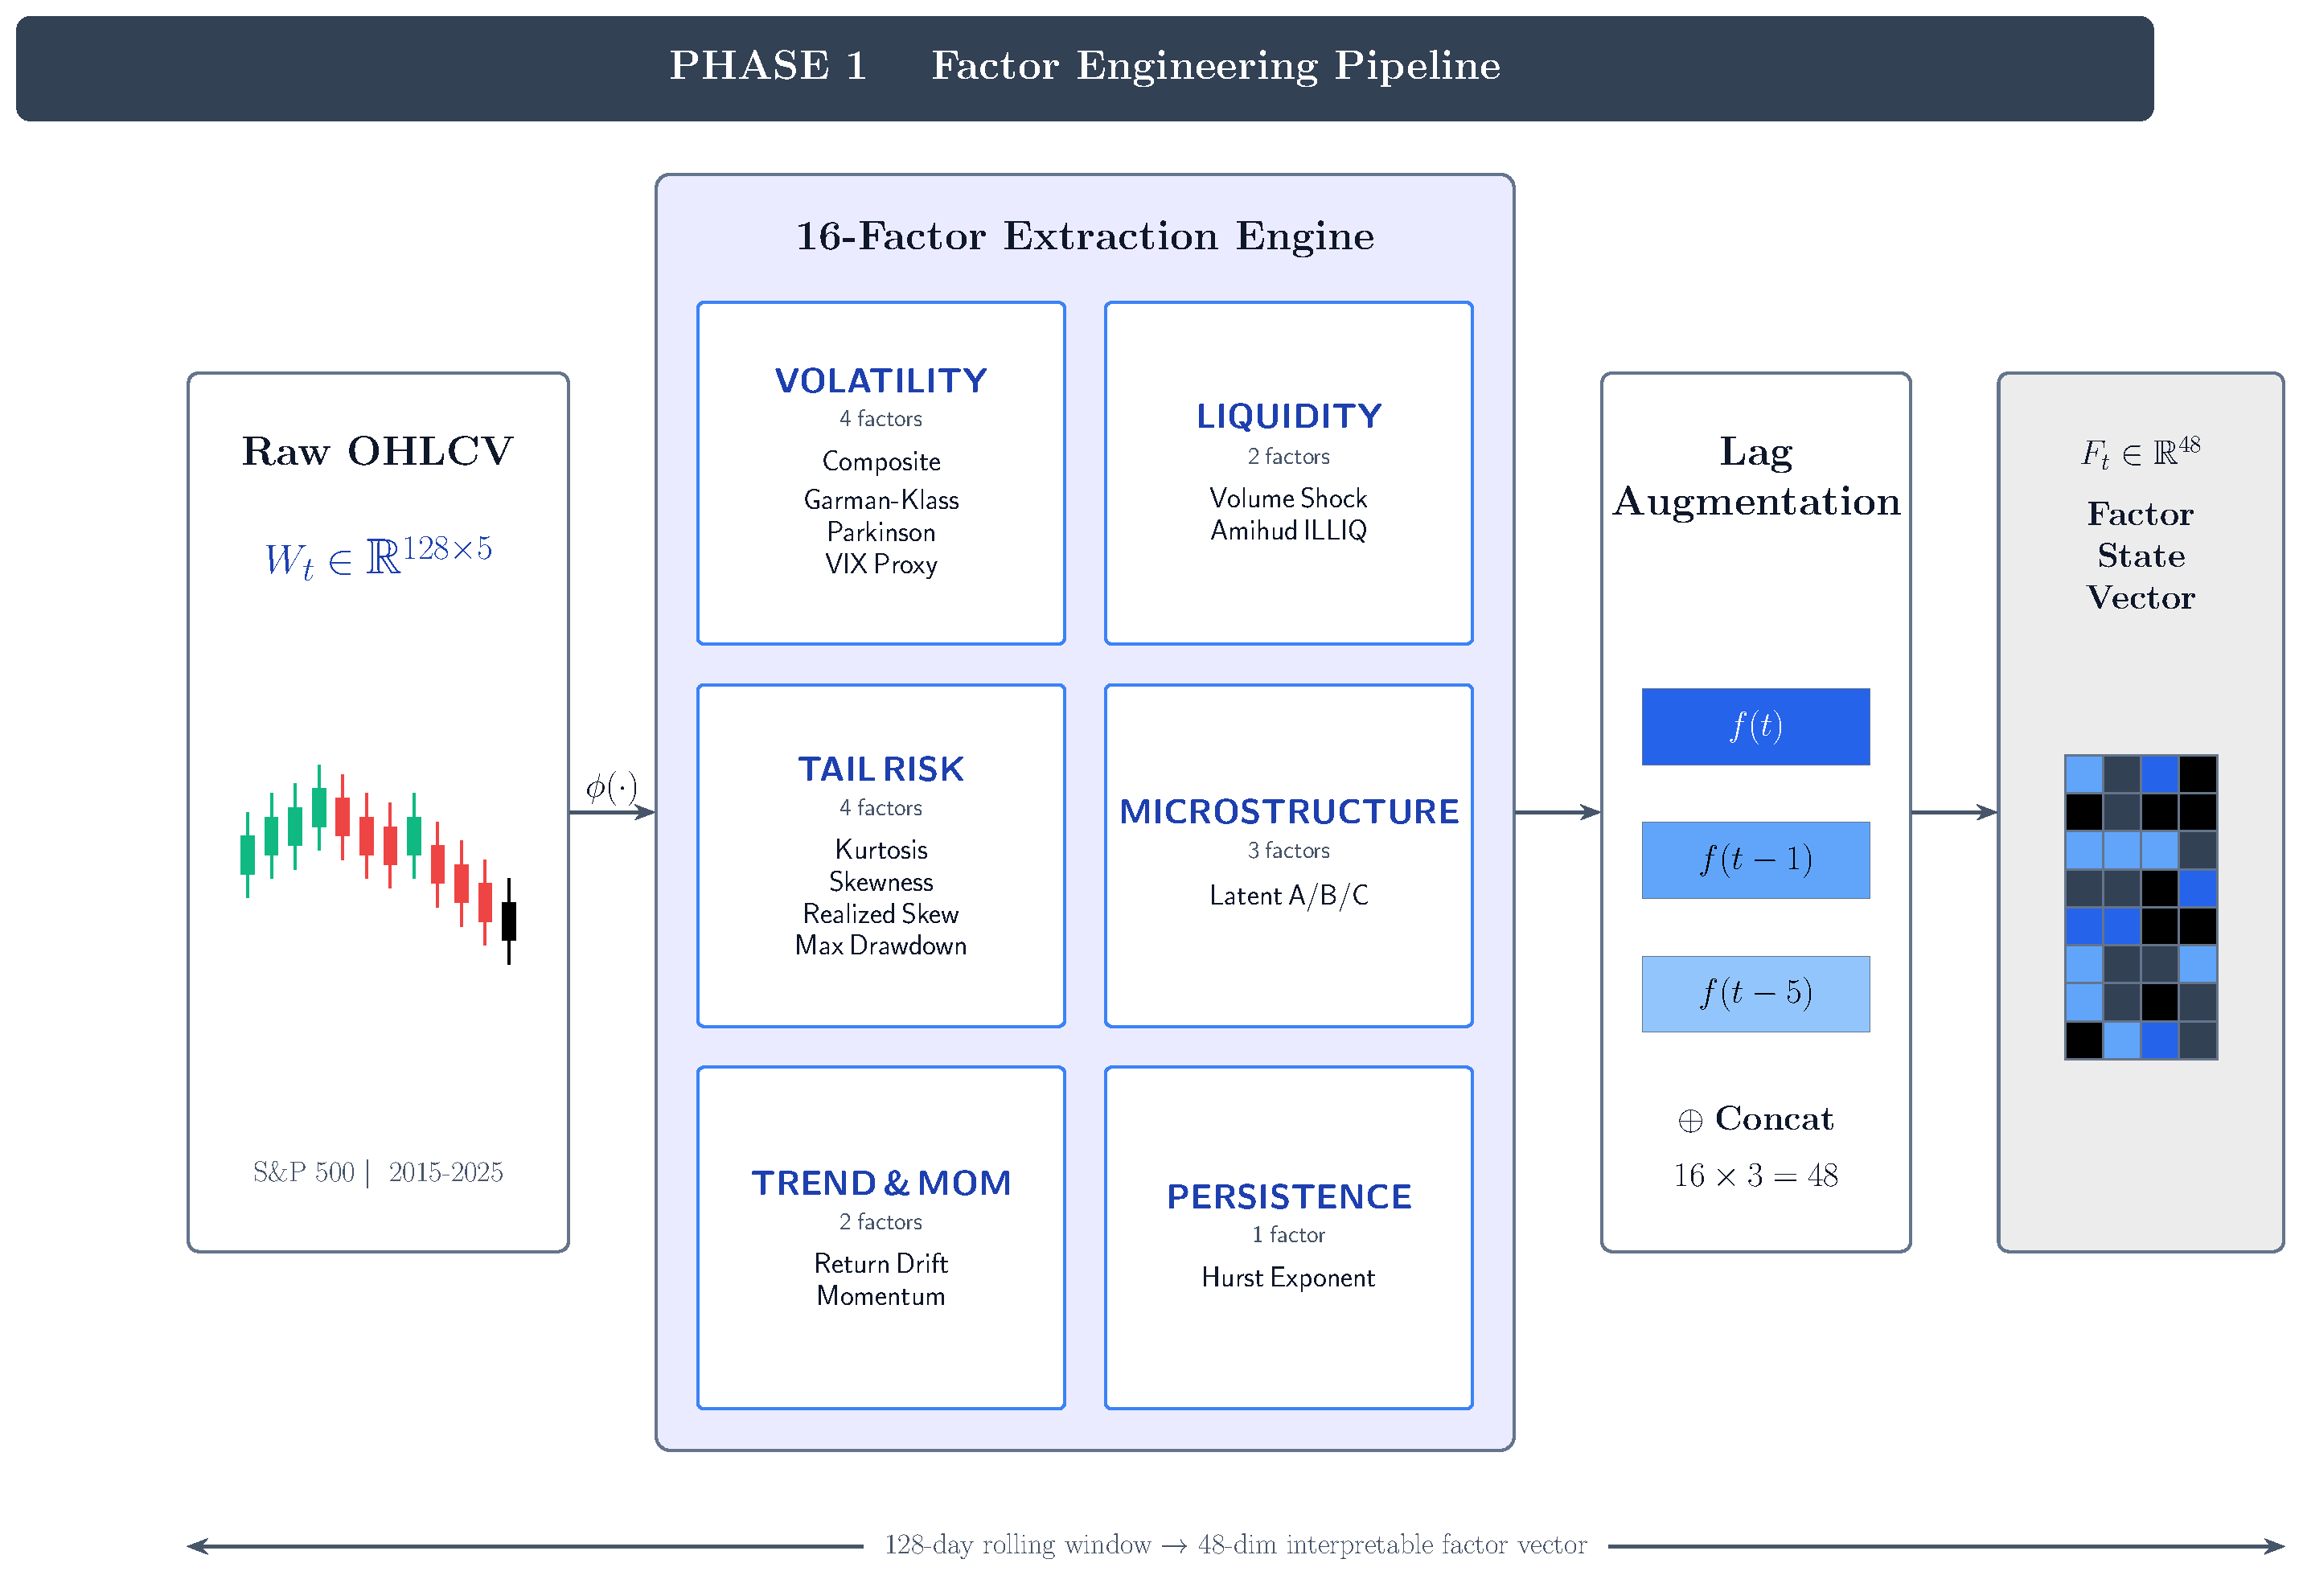
\includegraphics[width=1\textwidth]{final_figures/phase-1.pdf}
\caption{Phase 1: Factor Engineering Pipeline. A compact set of market factors, augmented with temporal lags, captures key dynamics such as trend, momentum, volatility, and tail risk for anomaly detection.}
\label{fig:phase1_pipeline}
\end{figure*}

Table~\ref{tab:factor_summary} summarizes the full library of factors grouped by economic type. For all of our experiments, we use a subset of eight factors (return trend, momentum, composite volatility, three latent-state factors, and the kurtosis and skewness tail factors). Further factors of range-based volatility, liquidity, and persistence estimates are introduced here for completeness, forming the full library that is fully evaluated in future research. Below we provide a description of all factors from the entire library, and mark eight key factors used in Table~\ref{tab:factor_summary}.

Trend and Momentum: Return Trend refers to the trend over a medium-term period and is defined as:
\begin{equation}
    \text{Trend}_t = \frac{1}{L} \sum_{i=1}^{L} r_{t-i+1}
\end{equation}
This measure is more responsive to consecutive negative returns before crashes. Momentum is the factor that represents directional persistence through an RSI-like proxy:
\begin{equation}
    \text{Mom}_t = \frac{\sum_{i=1}^{L} \max(r_{t-i+1}, 0)}{\sum_{i=1}^{L} |r_{t-i+1}|}
\end{equation}
which captures exhaustion in panic selloffs~\citep{cont2001empirical}.

Volatility: Composite Volatility is one of the most important factors that reflects general market volatility through the standard deviation within the window and is used as the regime assignment variable as defined in~\eqref{eq:volatility}. Three additional volatility estimators are added to the library. Garman--Klass volatility estimator makes use of intraday range information:
\begin{equation}
\begin{split}
    \text{GK}_t = \Biggl(\frac{1}{L}\sum_{i=1}^{L}\Bigl[0.5\,\log(H_i/\mathrm{Lo}_i)^2 \\
    - (2\ln 2 - 1)\log(C_i/O_i)^2\Bigr]\Biggr)^{\!1/2},
\end{split}
\label{eq:garman_klass}
\end{equation}
where $H_i$, $\mathrm{Lo}_i$, $O_i$, $C_i$ denote the high, low, open, and close within each sub-period. The Parkinson estimator \citep{parkinson1980extreme} provides a range-based alternative:
\begin{equation}
    \text{Park}_t = \sqrt{ \frac{\sum_{i=1}^{L} \log(H_i/\mathrm{Lo}_i)^2}{4L\ln 2} }
\end{equation}
which is more robust during low-volume periods. A VIX proxy approximates implied volatility as the ratio of 20-day ATR to the mean price level.

Tail Risk: two core factors capture distributional extremes. Excess kurtosis measures tail heaviness as:
\begin{equation}
    \text{Kurt}_t = \frac{\mathbb{E}[(r-\mu)^4]}{\sigma^4} - 3
\end{equation}
reflecting the heavy-tailed nature of financial return distributions \citep{bouchaud2001more}, and skewness quantifies return asymmetry, with negative values indicating crash-prone left tails. The extended library adds realized skewness, a within-window complement computed directly from the return series, and maximum drawdown, which captures the worst-case loss within each window:
\begin{equation}
    \text{MDD}_t = \max_{s < u \le L} \frac{\sum_{i=1}^{s} r_i - \sum_{i=1}^{u} r_i}{\max_{j \le s} \sum_{i=1}^{j} r_i + \epsilon},
    \label{eq:max_drawdown}
\end{equation}
where $\epsilon$ is a small constant for numerical stability.

Liquidity (extended library): volume shock measures abnormal trading volume relative to a rolling mean:
\begin{equation}
    \text{VShock}_t = \frac{V_t - \bar{V}_{t-20:t}}{\bar{V}_{t-20:t}}
\end{equation}
capturing institutional flow anomalies. The Amihud illiquidity ratio \citep{amihud2002illiquidity} quantifies price impact per unit volume:
\begin{equation}
    \text{ILLIQ}_t = \frac{1}{L} \sum_{i=1}^{L} \frac{|r_i|}{V_i + \epsilon},
    \label{eq:amihud}
\end{equation}
where high values indicate illiquid conditions with elevated slippage risk.

Microstructure and Persistence: three core latent-state factors are derived from the non-Close OHLCV data channels, capturing hidden market dynamics not directly observable from the close price alone. \emph{Latent State A} encodes the normalized overnight gap return:
\begin{equation}
    r^{\text{gap}}_t = \frac{O_t - C_{t-1}}{C_{t-1}}
\end{equation}
capturing after-hours information asymmetry and gap risk that frequently precede intraday trend continuation or reversal; large overnight gaps are a known precursor to elevated intraday volatility. \emph{Latent State B} is an intraday directional pressure index computed as the high-to-open gain normalized by the full intraday range:
\begin{equation}
    \text{LS\_B}_t = \frac{H_t - O_t}{H_t - \mathrm{Lo}_t + \varepsilon}
\end{equation}
reflecting the balance of buying versus selling pressure within each sub-period; values approaching 1 (0) signal sustained buying (selling) dominance and are associated with momentum continuation anomalies. \emph{Latent State C} is a range-based microstructure liquidity proxy, the normalized High--Low spread relative to the rolling 20-period Average True Range:
\begin{equation}
    \text{LS\_C}_t = \frac{H_t - \mathrm{Lo}_t}{\mathrm{ATR}_{20,t} + \varepsilon}
\end{equation}
elevated values indicate reduced market depth and increased execution risk, consistent with the flash-crash and order-book imbalance dynamics that dominate low-volatility anomalies (Section~\ref{subsec:eci}). The extended library further adds the Hurst exponent, estimated via rescaled range (R/S) analysis, which distinguishes mean-reverting ($H < 0.5$), random walk ($H \approx 0.5$), and trending ($H > 0.5$) behavior within each window, providing a direct measure of regime persistence.

To incorporate limited temporal context without sequence models, each of the eight core factors is augmented with one-day and five-day lags, yielding the 24-dimensional model input~\eqref{eq:factor}:
\begin{equation}
    F_t = \bigl[\, f_t,\; f_{t-1},\; f_{t-5} \,\bigr]
    \in \mathbb{R}^{24}.
    \label{eq:factor}
\end{equation}

The factor extraction pipeline transforms the raw OHLCV sequences into the 24-dimensional core factor space; the successful separation of crisis vs. normal states in this projection is proof that the compact representation maintains the discriminative information necessary for regime-dependent anomaly detection. By using factor representations instead of raw sequences, our approach makes the structure of the market explicit without any of the noise, and retains information about return size, which is normally lost during deep learning because of normalization. This compact yet informative representation forms the inputs for the regime-dependent Mixture of Experts approach, whose regime detection and routing architecture is depicted in Fig.~\ref{fig:phase2_regime}.

\begin{figure*}[!t]
\centering
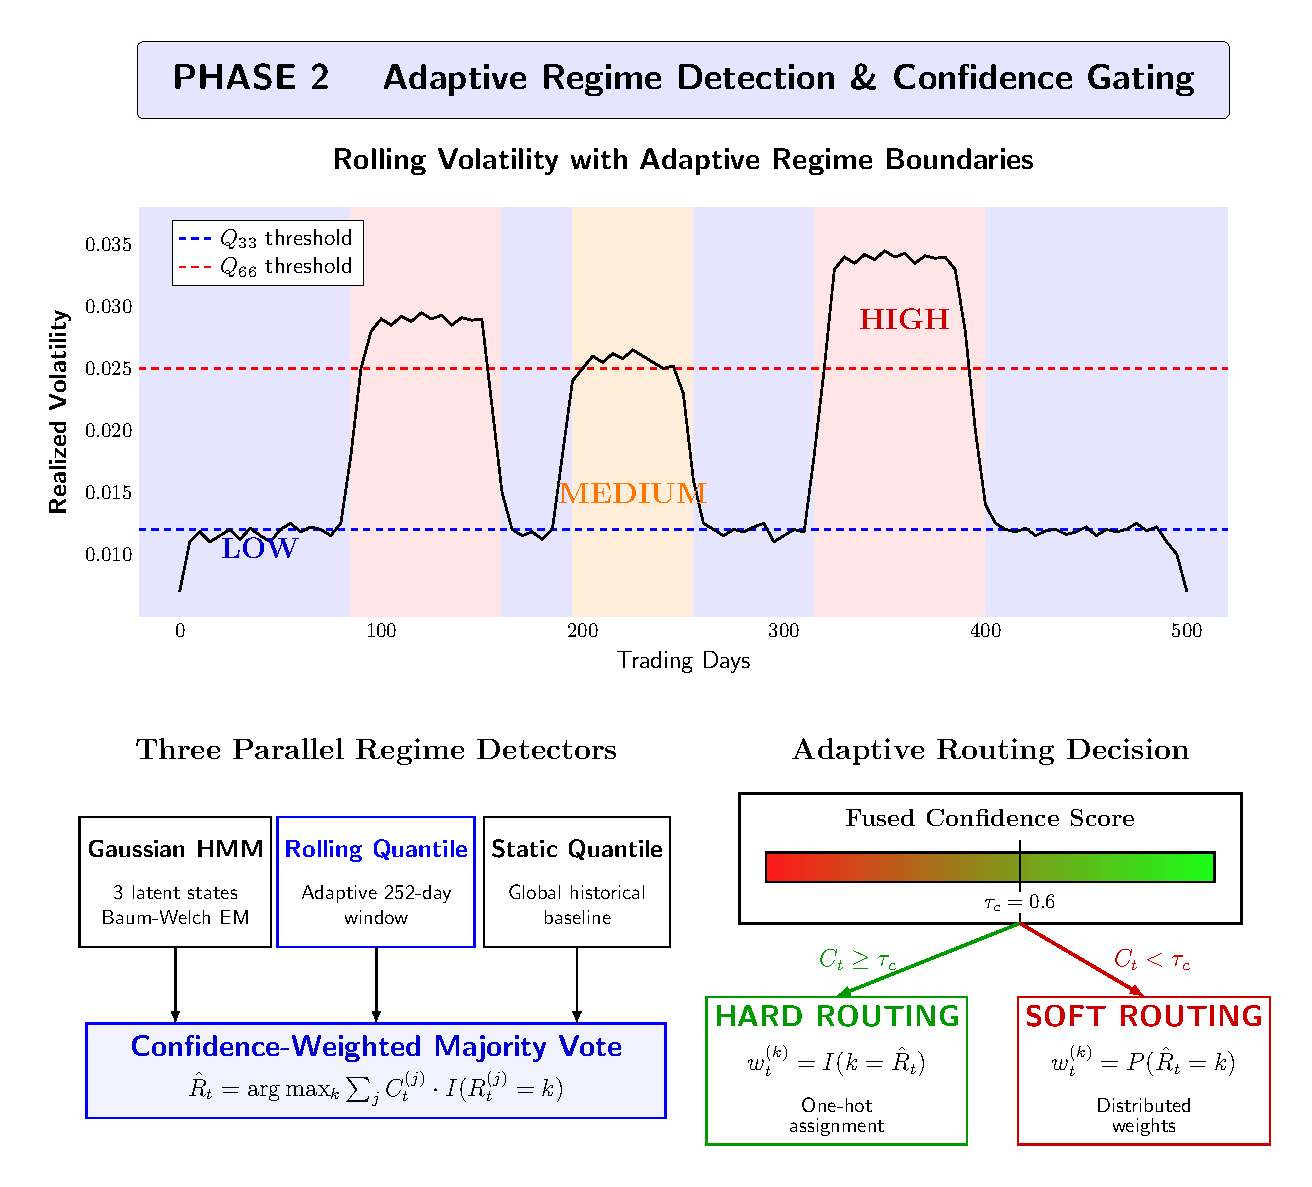
\includegraphics[width=1\textwidth, height=0.58\textheight, keepaspectratio=false]{final_figures/phase-2.pdf}
\caption{Phase 2: Adaptive Regime Detection and Routing System. A confidence-weighted fusion of multiple regime detectors identifies market states and dynamically routes inputs to the most appropriate regime-specific expert ensembles.}
\label{fig:phase2_regime}
\end{figure*}

\subsection{Regime-Conditioned Mixture of Experts}
\label{sec:moe}
Financial markets do not have a unique stationary data-generation process \citep{hamilton1989a}. A global classifier, designed to work in all volatility regimes, would need to consider the statistical properties of calm and turbulent markets, which leads to clashing decision boundaries and poor differentiation between normal and abnormal cases. To overcome this problem, we propose a regime-aware Mixture of Experts (MoE), where each expert handles one volatility regime. The conditional return distribution factorizes into~\eqref{eq:mixture}:
\begin{equation}
    P(r \mid F) =
    \sum_{k=1}^{K} P(r \mid F, R = k)\, P(R = k),
    \label{eq:mixture}
\end{equation}
where $R$ is the latent market regime. Standard anomaly detectors implicitly collapse this mixture into a single decision function, disregarding regime heterogeneity. The proposed framework instead estimates the regime-aware anomaly probability $P(A \mid F, R)$ directly. The complete MoE architecture is illustrated in Figure~\ref{fig:phase3_moe}.

\begin{figure*}[!t]
\centering
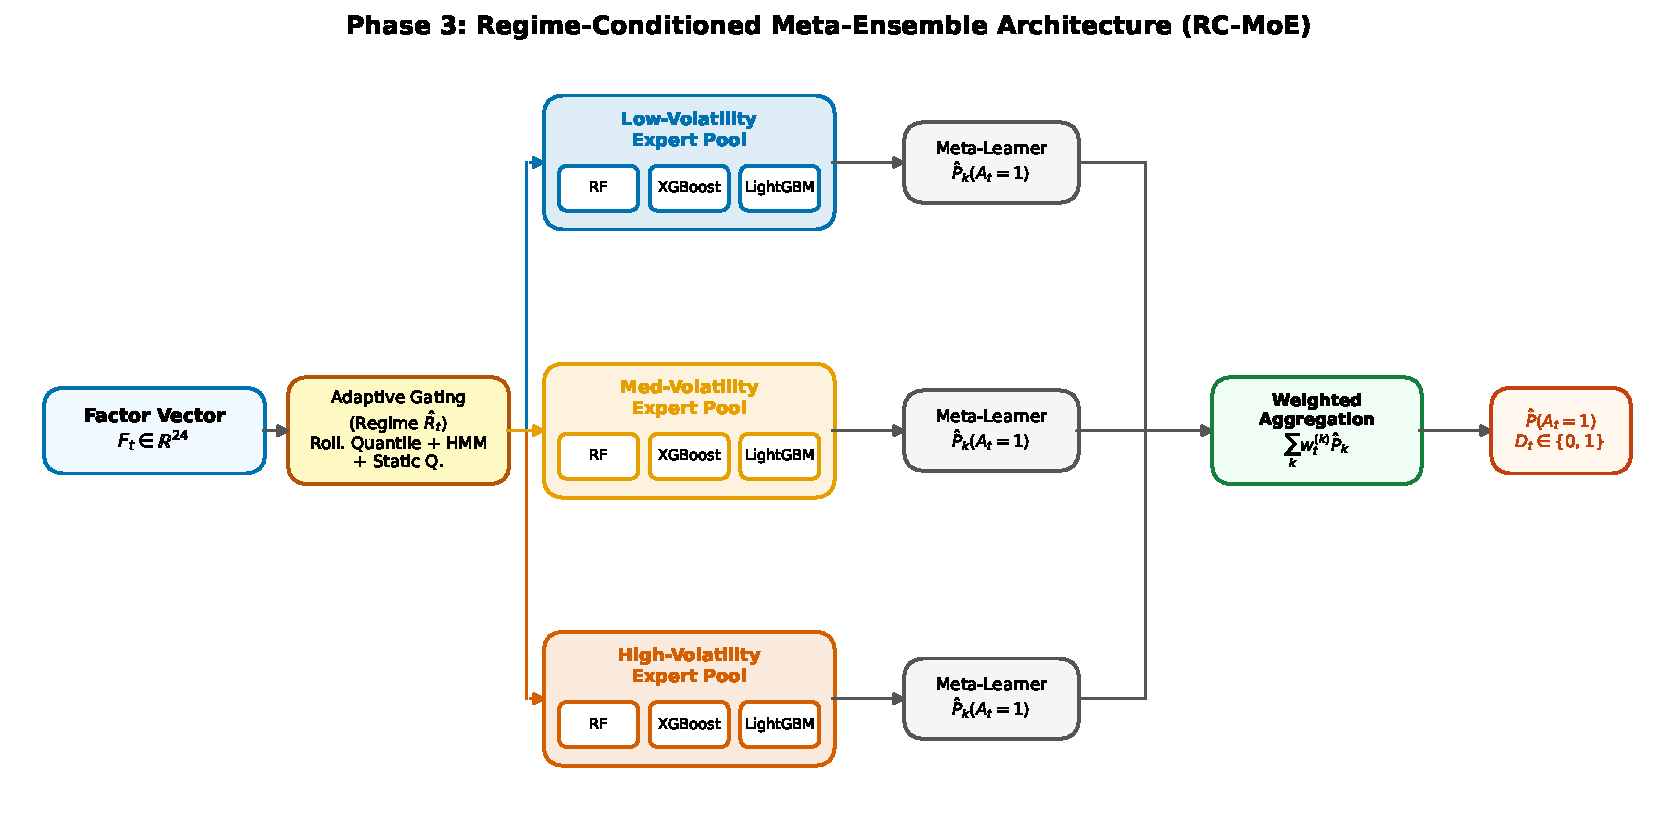
\includegraphics[width=1\textwidth ]{final_figures/phase-3.png}
\caption{Phase 3: Meta-Ensemble Learning Architecture Conditioned on Regimes.
Adaptive gates route inputs to volatility-specific expert ensembles, whose predictions
are combined through regime-specific meta-learners to generate final anomaly
probability scores.}
\label{fig:phase3_moe}
\end{figure*}

\subsubsection{Gating Mechanism}

The gating function maps each window to a regime label via the adaptive multi-detector fusion mechanism described in Section~\ref{sec:regime_definition}. The fused regime assignment~\eqref{eq:gating} is:
\begin{equation}
    R_t = g(\sigma_t) = \hat{R}_t,
    \label{eq:gating}
\end{equation}
where $\hat{R}_t$ is determined by the confidence-weighted voting rule defined in~\eqref{eq:fusion}. When all three detectors agree (high fused confidence $C_t \geq 0.6$), a hard, interpretable assignment is produced, preventing information leakage between experts during training and ensuring that each expert optimizes its decision boundary solely against the distributional characteristics of its assigned regime. In the ambiguous case ($C_t < 0.6$), soft routing distributes the observation to neighboring experts as specified in~\eqref{eq:routing}, providing a principled mechanism for handling regime transitions.

\subsubsection{Expert Models}

Each regime $k \in \{0, 1, 2\}$ is handled by a pool of $M$ independent experts trained exclusively on observations from that regime. Each expert $E_k^{(m)}$ produces a probability estimate~\eqref{eq:expert}:
\begin{equation}
    E_k^{(m)} : F_t \rightarrow \hat{P}^{(m)}(A_t = 1 \mid F_t, R_t = k),
    \label{eq:expert}
\end{equation}
where $m \in \{1, \ldots, M\}$ indexes the expert model family. Six distinct model families are employed per regime, spanning both tabular and sequential inductive biases.

Tree-Based Experts: Three complementary tree ensemble families provide the foundation. Random Forest classifiers with $n_{\text{estimators}} = 200$ and maximum depth of 5 serve as baseline experts, with class-balanced sample weighting to handle the approximately 2\% anomaly prevalence \citep{breiman2001random}. XGBoost experts \citep{chen2016xgboost} employ gradient boosting with $n_{\text{estimators}} = 200$, maximum depth of 5, $L_1$ regularization ($\alpha = 0.1$), $L_2$ regularization ($\lambda = 1.0$), and auto-computed scale\_pos\_weight to address class imbalance. LightGBM experts \citep{ke2017lightgbm} use leaf-wise (best-first) tree growth with $n_{\text{estimators}} = 200$, $\text{num\_leaves} = 31$, and the is\_unbalance flag for automatic class weighting. The gradient boosting architectures provide complementary inductive biases to Random Forest, with built-in regularization preventing overfitting on the small per-regime sample sizes.

\subsubsection{Explored Architectures (Not Evaluated in Reported Results)}
\label{subsubsec:explored}

The following three deep-learning expert families were implemented and trained but, as noted above, did not exceed the tree-based experts under the sparse per-regime sample sizes; they are documented here for architectural completeness and are excluded from every result reported in this paper.

Regime-Aware Temporal Attention Network (RA-TAN): A Transformer-based architecture injects regime-specific knowledge into the attention mechanism. The raw sequence $X_t \in \mathbb{R}^{L \times F}$ is projected to a $d_{\text{model}}$-dimensional space, and positional encodings are augmented with learned regime embeddings~\eqref{eq:ratan_input}:
\begin{equation}
    Z_t^{(0)} = X_t W_{\text{proj}} + \text{PE}_{1:L} + \mathbf{e}_{R_t},
    \label{eq:ratan_input}
\end{equation}
where $\mathbf{e}_{R_t} \in \mathbb{R}^{d_{\text{model}}}$ is a learned embedding for regime $R_t$ and $\text{PE}_{1:L}$ denotes sinusoidal positional encodings. The regime embedding is broadcast across all time steps, conditioning the subsequent multi-head self-attention layers to learn regime-specific temporal dependencies. Three Transformer encoder layers with $n_{\text{heads}} = 4$ and $d_{\text{model}} = 64$ process the regime-conditioned sequence, and the final representation is mean-pooled across the temporal dimension before classification.

GRU-Attention Expert: A bidirectional Gated Recurrent Unit with multi-head attention captures sequential dependencies without regime embedding. The architecture employs 2-layer bidirectional GRU ($d_{\text{hidden}} = 64$) followed by a $4$-head attention mechanism that produces a context vector for classification.

Hybrid Expert: A dual-branch model that fuses the factor vector and the raw sequence through a cross-attention layer, combining the tabular and sequential representations into a single classifier.

All deep learning experts are trained with a focal loss function \citep{lin2017focal} to address the severe class imbalance~\eqref{eq:focal}:
\begin{equation}
    \mathcal{L}_{\text{focal}} = -\alpha_t (1 - p_t)^{\gamma} \log(p_t),
    \label{eq:focal}
\end{equation}
with $\alpha = 0.75$ and $\gamma = 2.0$, which down-weights well-classified normal samples and concentrates gradient signal on hard-to-classify boundary cases.

\begin{figure*}[!t]
\centering
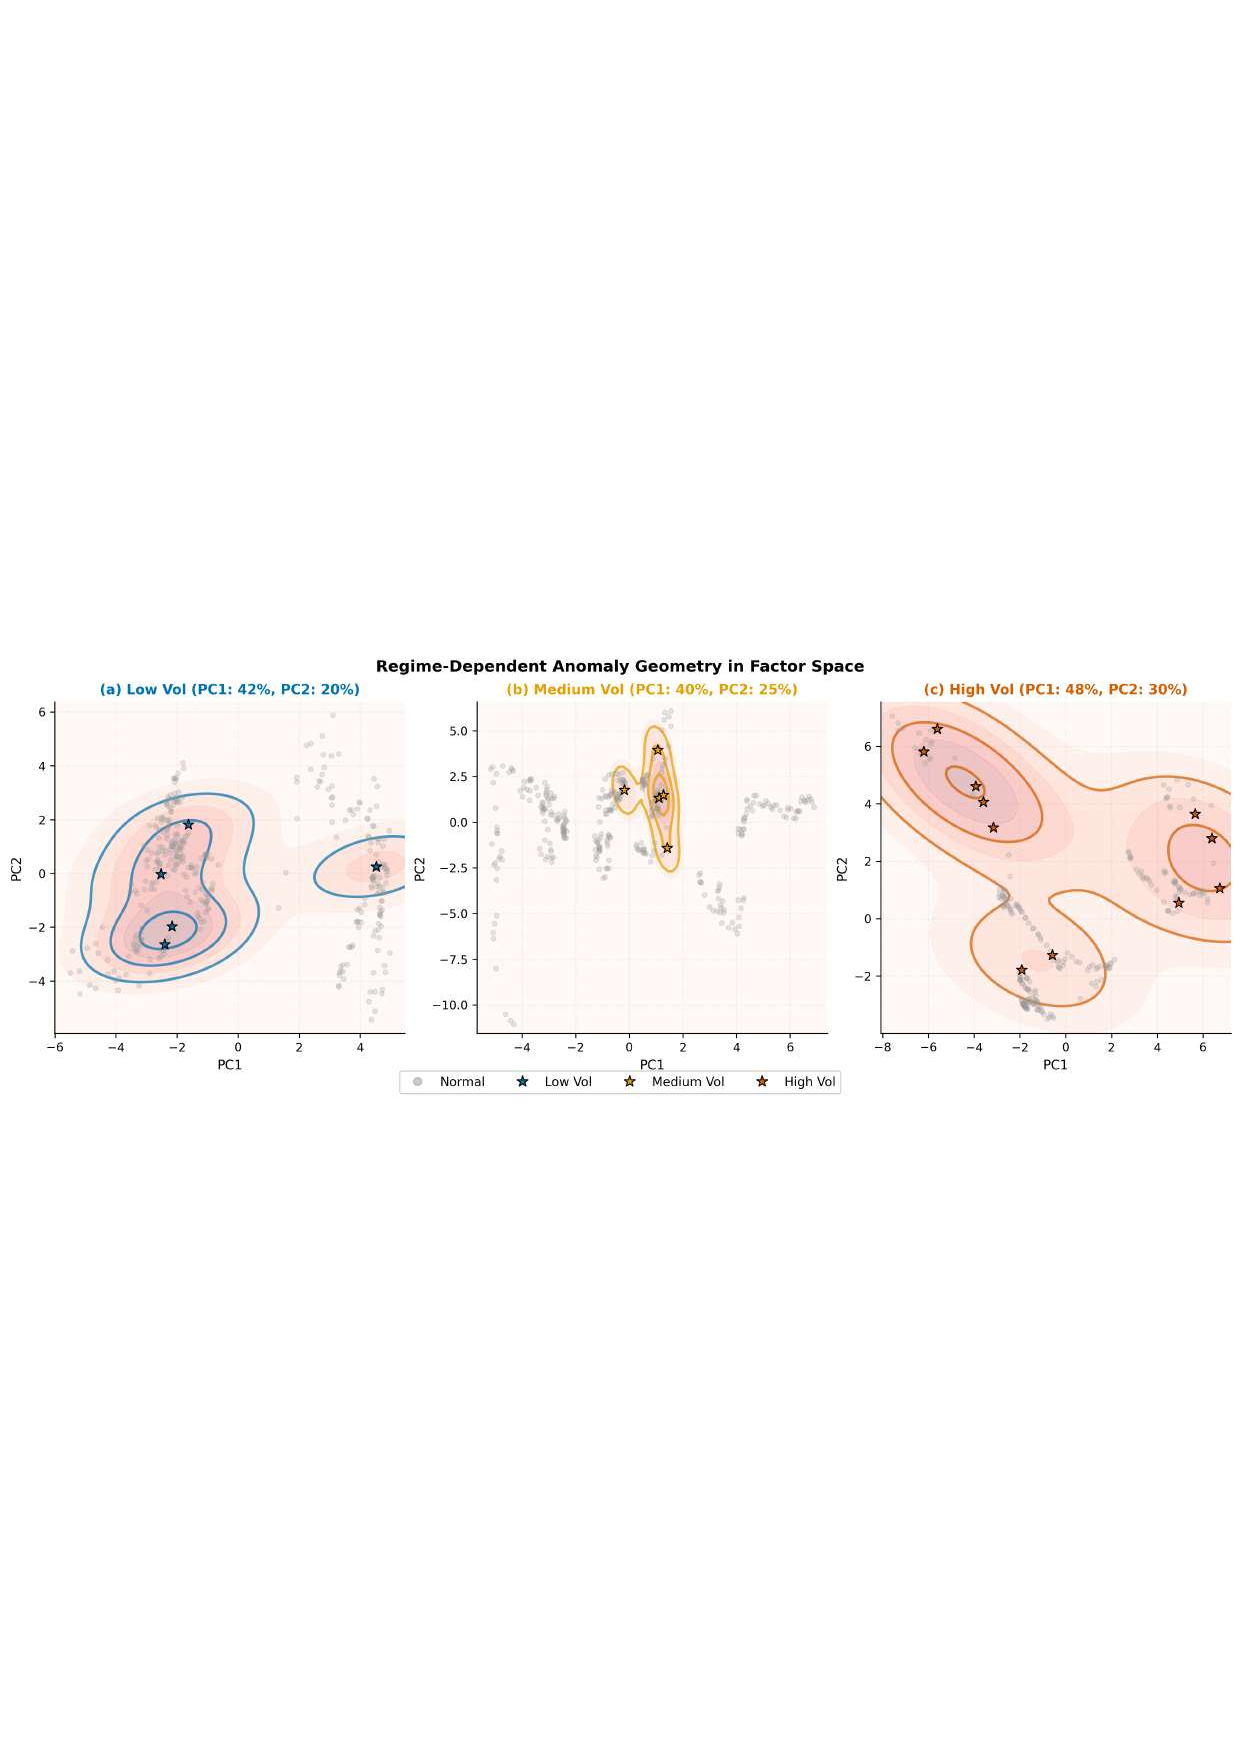
\includegraphics[width=0.98\textwidth]{final_figures/fig_m3_topological_boundaries.png}
\caption{Dependent regime anomaly boundaries: There is substantial variation in anomaly behavior among volatility regimes, indicating that there cannot be just one decision boundary for all.
}
\label{fig:topological_boundaries}
\end{figure*}

Fig.~\ref{fig:topological_boundaries} shows the learned decision boundaries for each of the three regime-specific expert pools. The qualitatively distinct geometries across the three regime panels indicate that anomaly structure is regime-dependent: anomalies in the low-volatility regime are concentrated at extreme momentum values, whereas in the high-volatility regime they span a broader range of return trends, a separation that a single global classifier would tend to compromise.

This regime dependence is also visible directly in the feature space. Figure~\ref{fig:regime_tsne} projects the 24-factor windows into two dimensions via t-SNE and overlays the per-regime return-trend densities: anomalies (stars) occupy regime-specific sub-regions, and the return distribution broadens and shifts markedly from the low- to the high-volatility regime. Figure~\ref{fig:regime_patterns} complements this with representative $128$-day price/volume windows drawn from each regime, illustrating the visually distinct micro-structure, calm drifts in low-volatility windows versus clustered, high-amplitude moves in high-volatility windows.

\begin{figure*}[!t]
  \centering
  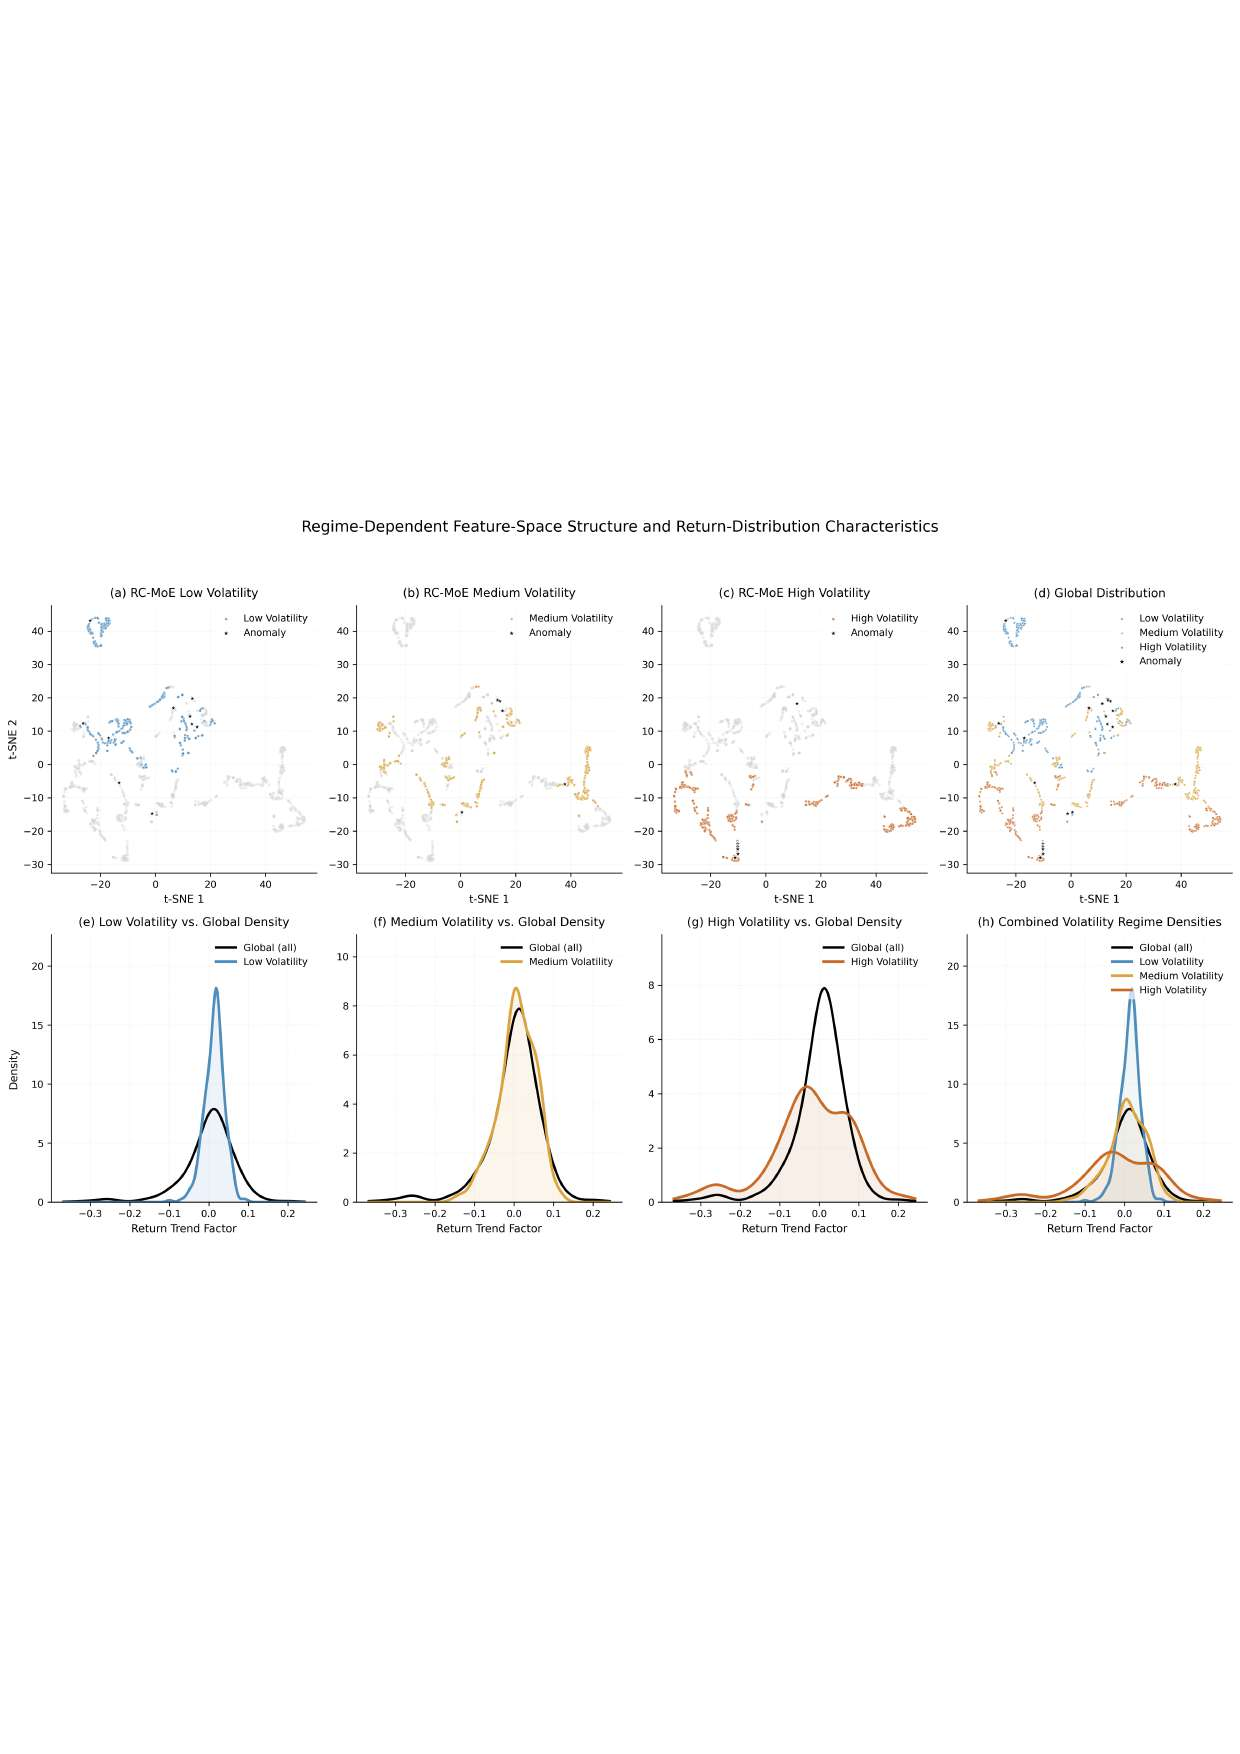
\includegraphics[width=0.98\textwidth]{final_figures/fig3_regime_tsne_kde.png}
  \caption{Anomalies have different behaviors within different volatility regimes, and there are anomalies and return distribution patterns in low, medium, and high volatility regimes.
}
  \label{fig:regime_tsne}
\end{figure*}

\begin{figure*}[!t]
  \centering
  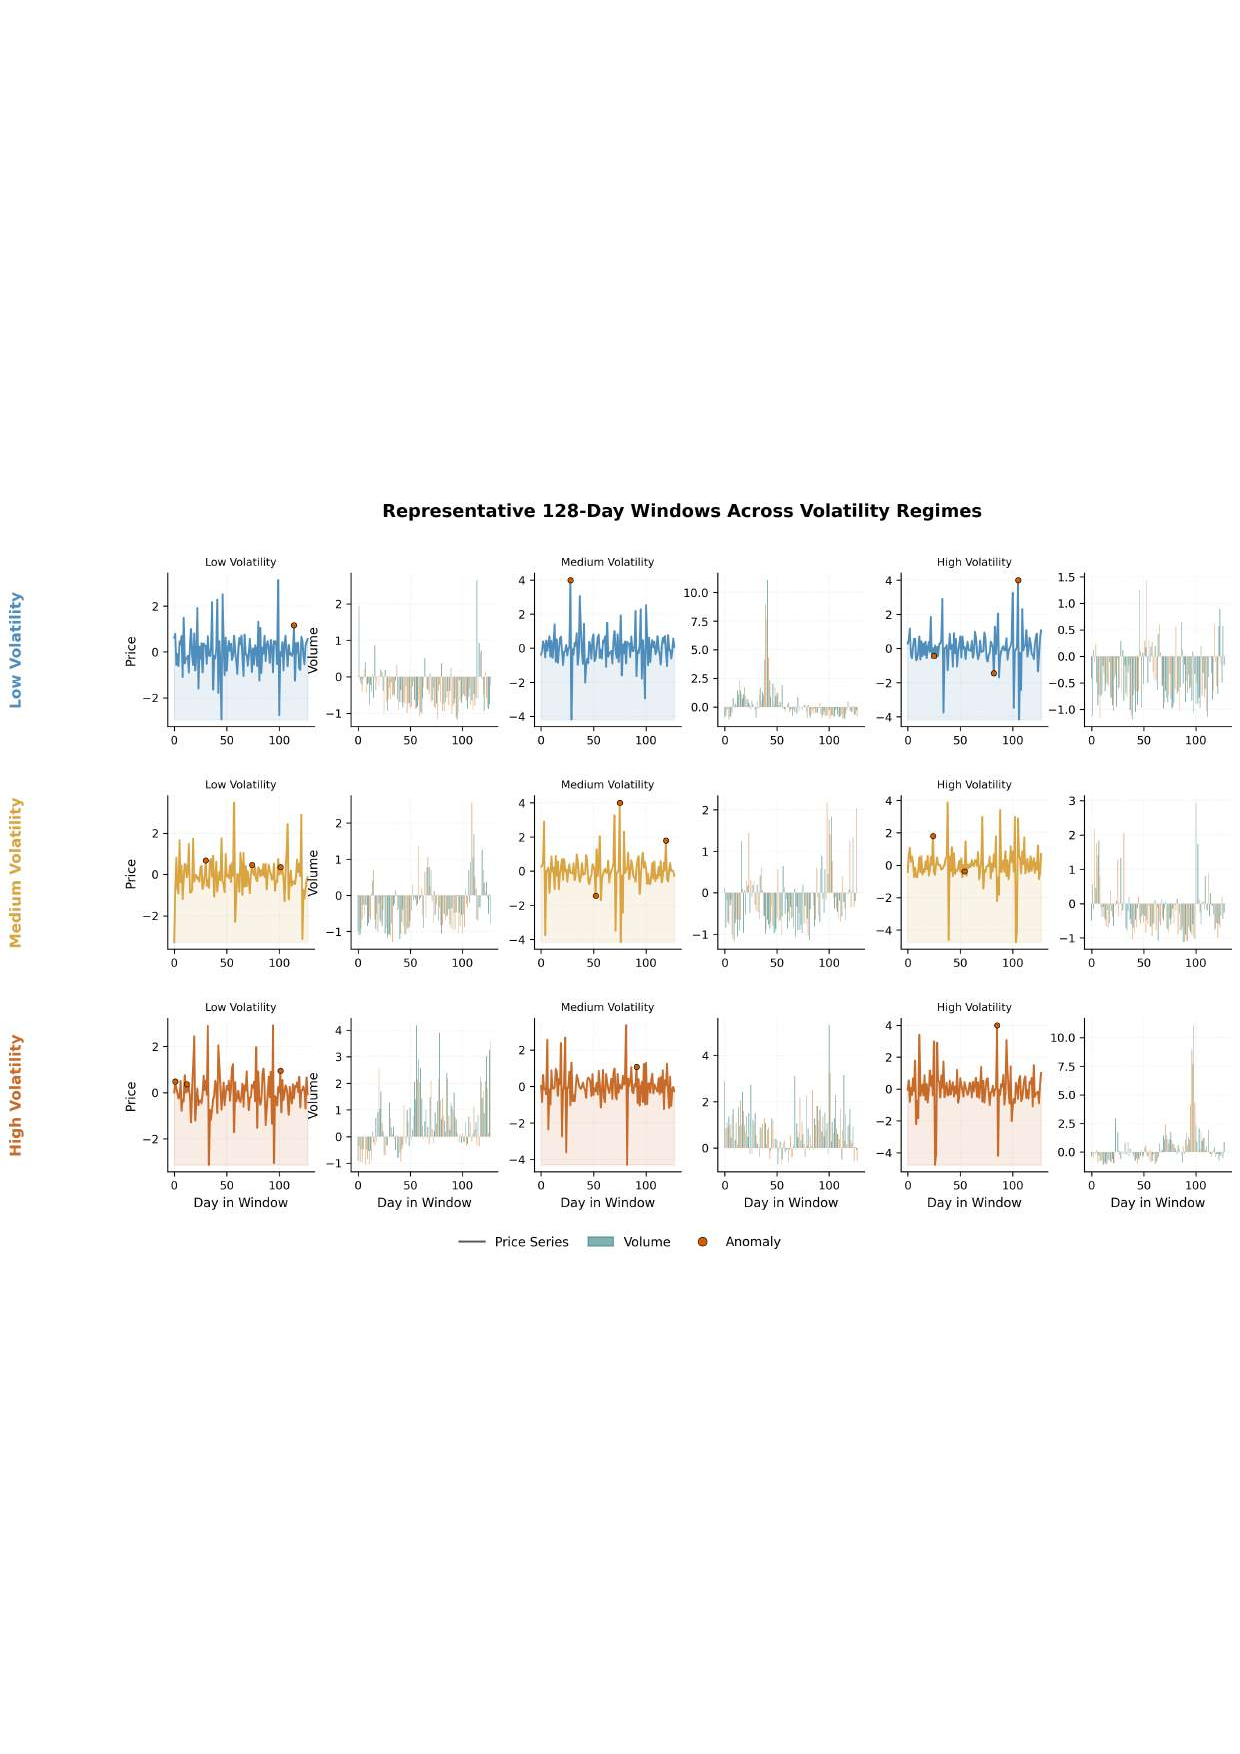
\includegraphics[width=0.98\textwidth]{final_figures/fig6_regime_patterns.png}
  \caption{Windows from various volatilities display different characteristics in prices, anomalies, and volumes, proving the necessity of using expert models on each regime separately.
}
  \label{fig:regime_patterns}
\end{figure*}

\subsubsection{Inference Procedure}

At inference time, a new window $W_t$ is processed through seven sequential steps: factor extraction, volatility estimation, multi-detector regime identification, confidence-weighted fusion, adaptive routing, per-regime expert evaluation, and meta-ensemble stacking. The complete procedure is formalized in Algorithm~\ref{alg:moe_inference}. The final calibrated anomaly probability is produced by a Level-2 meta-learner that fuses the outputs of all $M$ experts active in the assigned regime:
\begin{algorithm}[htb]
\caption{Regime-Conditioned Meta-Ensemble: Inference}
\label{alg:moe_inference}
\begin{algorithmic}[1]
\raggedright % Disables the ugly stretching/justification without breaking the layout
\REQUIRE Window $W_t$, detectors $\{D_1, D_2, D_3\}$, expert pools $\{\mathcal{E}_k\}$, meta-learners $\{\text{Meta}_k\}$, $\tau_c = 0.6$
\ENSURE Calibrated anomaly probability $\hat{P}(A_t = 1)$, decision $D_t \in \{0,1\}$

\STATE \textbf{Factor extraction:} $F_t \leftarrow \phi(W_t) \in \mathbb{R}^{24}$

\STATE \textbf{Regime estimation:} $R_t^{(i)}, C_t^{(i)} \leftarrow D_i(\sigma_t)$ for $i \in \{1,2,3\}$

\STATE \textbf{Confidence-weighted fusion:}
\STATE \hspace{2em} $\hat{R}_t \leftarrow \arg\max_k \sum_i C_t^{(i)} \cdot \mathbb{I}(R_t^{(i)} = k)$;\ $C_t \leftarrow \max_k P(\hat{R}_t = k)$

\STATE \textbf{Adaptive routing:}
\IF{$C_t \geq \tau_c$}
    \STATE $w_t^{(k)} \leftarrow \mathbb{I}(k = \hat{R}_t)$ \hfill \{Hard routing\}
\ELSE
    \STATE $w_t^{(k)} \leftarrow P(\hat{R}_t = k)$ \hfill \{Soft routing\}
\ENDIF

\STATE \textbf{Expert evaluation:} $\hat{p}_k^{(m)} \leftarrow E_k^{(m)}(F_t)$\ for active $k$ ($w_t^{(k)}>0$), all $m$

\STATE \textbf{Meta-ensemble stacking:}
\STATE \hspace{2em} $\hat{P}_k(A_t\!=\!1) \leftarrow \text{Meta}_k\!\left(\hat{p}_k^{(1)}, \ldots, \hat{p}_k^{(M)}\right)$

\STATE \textbf{Final probability:} $\hat{P}(A_t\!=\!1) \leftarrow \sum_k w_t^{(k)} \hat{P}_k(A_t\!=\!1)$
\STATE \hspace{2em} $D_t \leftarrow \mathbb{I}\!\left(\hat{P}(A_t\!=\!1) \geq \tau\right)$,\ $\tau = 0.50$

\RETURN $\hat{P}(A_t = 1)$, $D_t$
\end{algorithmic}
\end{algorithm}

A global Random Forest baseline trained on the full dataset without regime partitioning is retained as a reference to quantify the benefit of regime conditioning. The tree-based experts maintain interpretability with shallow architectures (depth 5), and all quantitative comparisons, ablations, and the economic backtest reported in this paper are based exclusively on these tree-based experts (RF, XGBoost, and LightGBM). The deep-learning experts described in Section~\ref{subsubsec:explored} (RA-TAN, GRU-Attention, and the Hybrid cross-attention expert) were implemented and trained but, under preliminary per-regime evaluation with only $n\!\approx\!64$--$67$ validation observations per regime, did not exceed the tree-based experts; they are therefore excluded from all reported results and are documented for architectural completeness only. This is consistent with the paper's central thesis, that a structurally well-posed problem formulation, rather than model capacity, drives separability when labeled extreme events are scarce \citep{arrieta2020explainable}. Table~\ref{tab:model_complexity} reports the parameter counts of the evaluated tree experts alongside the explored deep architectures.

\begin{table}[t]
\tbl{Model complexity (evaluated: tree-based; excluded: deep architectures)}
{\footnotesize
\renewcommand{\arraystretch}{1.25}
\begin{tabular}{lccc}
\toprule
\textbf{Model} & \textbf{Input} & \textbf{Params} & \textbf{Type} \\
\midrule
\multicolumn{4}{l}{\emph{Evaluated (all reported results)}} \\
Global RF              & $\mathbb{R}^{24}$         & $\sim 400$      & Tree        \\
RF/XGB/LGBM MoE        & $\mathbb{R}^{24}$         & $\sim 2{,}700$  & Tree        \\
\midrule
\multicolumn{4}{l}{\emph{Explored, not evaluated (Sec.~\ref{subsubsec:explored})}} \\
GRU-Attention (per reg.)& $\mathbb{R}^{128 \times F}$& $\sim 35{,}000$ & Sequence    \\
RA-TAN (global)         & $\mathbb{R}^{128 \times F}$& $\sim 28{,}000$ & Attention   \\
Hybrid Expert           & Dual-branch                & $\sim 42{,}000$ & Cross-Attn \\
\bottomrule
\end{tabular}}
\label{tab:model_complexity}
\end{table}

The regime-conditioned MoE acknowledges that anomaly mechanisms differ across volatility states. Separating regimes before training eliminates conflicting decision boundaries and lets each expert specialize within its assigned market environment. The meta-ensemble stacking layer further learns optimal per-regime combination weights, automatically down-weighting poorly calibrated experts. While regime isolation and diversified expertise together produce high in-sample separation, out-of-sample accuracy degrades owing to the non-stationarity of financial anomalies, a gap quantified in the next section.

% SECTION V - EXPERIMENTAL Setup
% ================================================================
\section{Experimental Setup}
\label{sec:experimental}

\subsection{Datasets}
\label{subsec:datasets}

All experiments use daily data over 2016--2025. The primary single-asset study is conducted on the S\&P~500; the multi-market replication of Section~\ref{subsubsec:multimarket} adds the NASDAQ Composite, the Russell~2000 small-cap index, and Bitcoin, chosen for their deliberately distinct microstructure and tail behaviour. Table~\ref{tab:datasets} summarises the four datasets. Each daily series is converted into overlapping 128-day windows, and anomalies are labelled at the 95th return-percentile (matching the $\text{VaR}_{95}$ tail definition of Section~\ref{subsubsec:evt}); every market is represented by the same eight-factor, 24-dimensional input.

\begin{table}[!t]
\tbl{Datasets (daily, 2016--2025; 8-factor 24-dim input; anomalies at 95th percentile)}
{\scriptsize
\renewcommand{\arraystretch}{1.25}
\setlength{\tabcolsep}{2.5pt}
\begin{tabular}{llp{1.7cm}rrr}
\toprule
\textbf{Market} & \textbf{Ticker} & \textbf{Asset class} & \textbf{Days} & \textbf{Win.} & \textbf{Anom.\ (\%)} \\
\midrule
S\&P 500     & \^{}GSPC   & Large-cap equity & 2513 & 2364 & 148 (6.3\%) \\
NASDAQ       & \^{}IXIC   & Tech equity      & 2513 & 2365 & 162 (6.8\%) \\
Russell 2000 & \^{}RUT    & Small-cap equity & 2513 & 2362 & 152 (6.4\%) \\
Bitcoin      & BTC-USD    & Crypto           & 3652 & 3504 & 165 (4.7\%) \\
\bottomrule
\end{tabular}}
\label{tab:datasets}
\end{table}

\subsection{Evaluation Framework}
\label{subsec:eval_framework}

Evaluation distinguishes between two modes of assessment with distinct scientific objectives~\citep{liu2024times, chandola2009anomaly}.

\subsubsection{Structural Separability (In-Sample)}
\label{subsubsec:in_sample}

Models receive expert training and evaluation within partitions defined by regimes without needing temporal generalization. Such an approach answers the diagnostic question: \emph{Are extreme events separable from other data within factor space based on regime information?} Such results should be viewed as an upper bound on structural separability given particular regime definition and serve merely as a diagnostic for regime-conditional separability.

\subsubsection{Predictive Generalization (Out-of-Sample)}
\label{subsubsec:out_of_sample}

The following three tests measure the ability to generalize temporally. The blocked temporal split separates each regime's data temporally in a 70-30 train-test split while maintaining the temporal order and avoiding any look-ahead bias. Walk-forward validation requires models to be trained on all available data until time $t$ and tested on the following period $t{+}1$. The window is then shifted and the process repeated. Such an approach provides the most rigorous test of predictive ability and approximates deployment settings more closely than any other setting. The five-fold temporal cross validation breaks up the entire evaluation period into 5 disjoint temporal folds where training takes place on folds $1, \ldots, k - 1$ while testing on fold $k$, where $k = \{2,3,4,5\}$, with the splits being strictly chronological and no randomization taking place at any point; the procedure is followed for all experiments in Section~\ref{sec:multimodel} and Table~\ref{tab:regime_conditioning}. The whole process without any leakage in training and evaluation is summarized in Algorithm~\ref{alg:walk_forward}.

\begin{algorithm}[!t]
\caption{Leakage-Free Walk-Forward Training and Evaluation}
\label{alg:walk_forward}
\begin{algorithmic}[1]
\REQUIRE Factor matrix $X\in\mathbb{R}^{N\times 24}$, labels $y$, regime stream $R$, folds $K{=}5$, purge $g{=}128$
\STATE $s \leftarrow \lfloor N/K \rfloor$; \quad initialise pooled predictions $\hat{y}_g, \hat{y}_m \leftarrow \emptyset$
\FOR{$k = 1$ \TO $K-1$}
  \STATE $\text{tr} \leftarrow [0, ks)$; \quad $\text{te} \leftarrow [ks{+}g,\; \min(ks{+}g{+}s, N))$ \COMMENT{purge gap removes overlap leakage}
  \STATE refit regime boundaries on $\text{tr}$ only; assign $R_{\text{tr}}, R_{\text{te}}$
  \STATE fit scaler on $X_{\text{tr}}$; transform $X_{\text{tr}}, X_{\text{te}}$
  \STATE train global ensemble (RF$+$XGB$+$LGBM) on $(X_{\text{tr}}, y_{\text{tr}})$; get $p^{g}$
  \STATE $\tau_g \leftarrow \arg\max_{\tau}\, F_\beta^{\mathrm{E}}(p^{g}_{\text{tr}} \!\ge\! \tau,\, y_{\text{tr}})$ \COMMENT{threshold tuned on training fold only}
  \FOR{regime $r \in \{0,1,2\}$}
    \IF{$|\{\text{tr}: R{=}r\}| < 10$ \OR\ positives $< 3$}
      \STATE expert$_r \leftarrow$ global model \COMMENT{sparse-regime fallback}
    \ELSE
      \STATE train regime-$r$ ensemble on the regime slice; tune $\tau_r$ on its training slice
    \ENDIF
  \ENDFOR
  \STATE route each test window by $R_{\text{te}}$ to its expert; collect $\hat{y}_g, \hat{y}_m$
\ENDFOR
\RETURN event-wise $\mathrm{F1}$, precision, recall, and McNemar$(\hat{y}_g,\hat{y}_m,y)$ on pooled predictions
\end{algorithmic}
\end{algorithm}

% ----------------------------------------------------------------
\subsection{Evaluation Metrics}
\label{subsec:metrics}
% ----------------------------------------------------------------

Accuracy is not provided since the task suffers from an extremely skewed class distribution. The following performance metrics will be used in all experiments below:

\begin{enumerate}[label=\arabic*., itemsep=3pt]
	\item Precision ($\mathcal{P}$): proportion of flagged samples that actually represent anomalies,
          $\mathcal{P} = \mathrm{TP}/(\mathrm{TP}+\mathrm{FP})$.

    \item Recall ($\mathcal{R}$): proportion of true anomalies detected by the classifier,
          $\mathcal{R} = \mathrm{TP}/(\mathrm{TP}+\mathrm{FN})$.

    \item F1 score ($\mathcal{F}_{1}$): harmonic mean of precision and recall values,
          $\mathcal{F}_{1} = {2\,\mathcal{P}\,\mathcal{R}}/{(\mathcal{P}+\mathcal{R})}$.

    \item Event-F1 ($\mathcal{F}_{1}^{\mathrm{E}}$): F1 score with tolerance of $\pm3$ trading-days,
       adhering to the common practice for detection of sparse point events~\citep{liu2024times}.
\end{enumerate}

In regard to risk management, Recall carries more importance: a failure to detect an extreme event is much more damaging than a false alarm.

% ----------------------------------------------------------------
\subsection{Statistical Considerations}
\label{subsec:statistical}
% ----------------------------------------------------------------
Since there are only $n < 60$ instances of anomalies observed per each regime within a decade-long analysis, confidence intervals and hypothesis testing methods lack statistical power in this case. For confidence intervals, we use the technique of circular block bootstrap for estimating them, where the bootstrap blocks consist of $b=20$ trading days. This helps us to preserve autocorrelation in financial returns. The results are reported per each regime sample size.

% ================================================================
% SECTION VI - ABLATION STUDY
% ================================================================
\section{Ablation Study}
\label{sec:ablation}

In order to gauge the role of each architectural feature in an incremental way, we conduct an ablation study where we sequentially remove or substitute individual components. All variants use the same dataset, abnormality labels, and regimes.
% ----------------------------------------------------------------
\subsection{Ablation Design}
\label{subsec:ablation_design}
% ----------------------------------------------------------------

Six variations of the models are considered for the entire decade period (2016-2025). The standard deviation rule involves a global threshold-based detector that employs a fixed rolling return volatility criterion. The Z-score model uses a global return distribution for determining thresholds by applying standard Z-scores. ConvVAE involves the training of convolutional variational autoencoder using raw 128-day return windows~\citep{neloy2024a}. Anomaly transformer is one of the latest advancements of deep learning models for detecting anomalies in time series~\citep{song2023anoma}. Global random forest is a Random Forest classifier~\citep{breiman2001random} based on 24 factors that have not been divided into regimes, used as a primary ML baseline model. RC-MoE (Proposed) model is the complete RC-MoE framework.
% ----------------------------------------------------------------
\subsection{Results}
\label{subsec:ablation_results}
% ----------------------------------------------------------------

\begin{figure*}[!t]
  \centering
  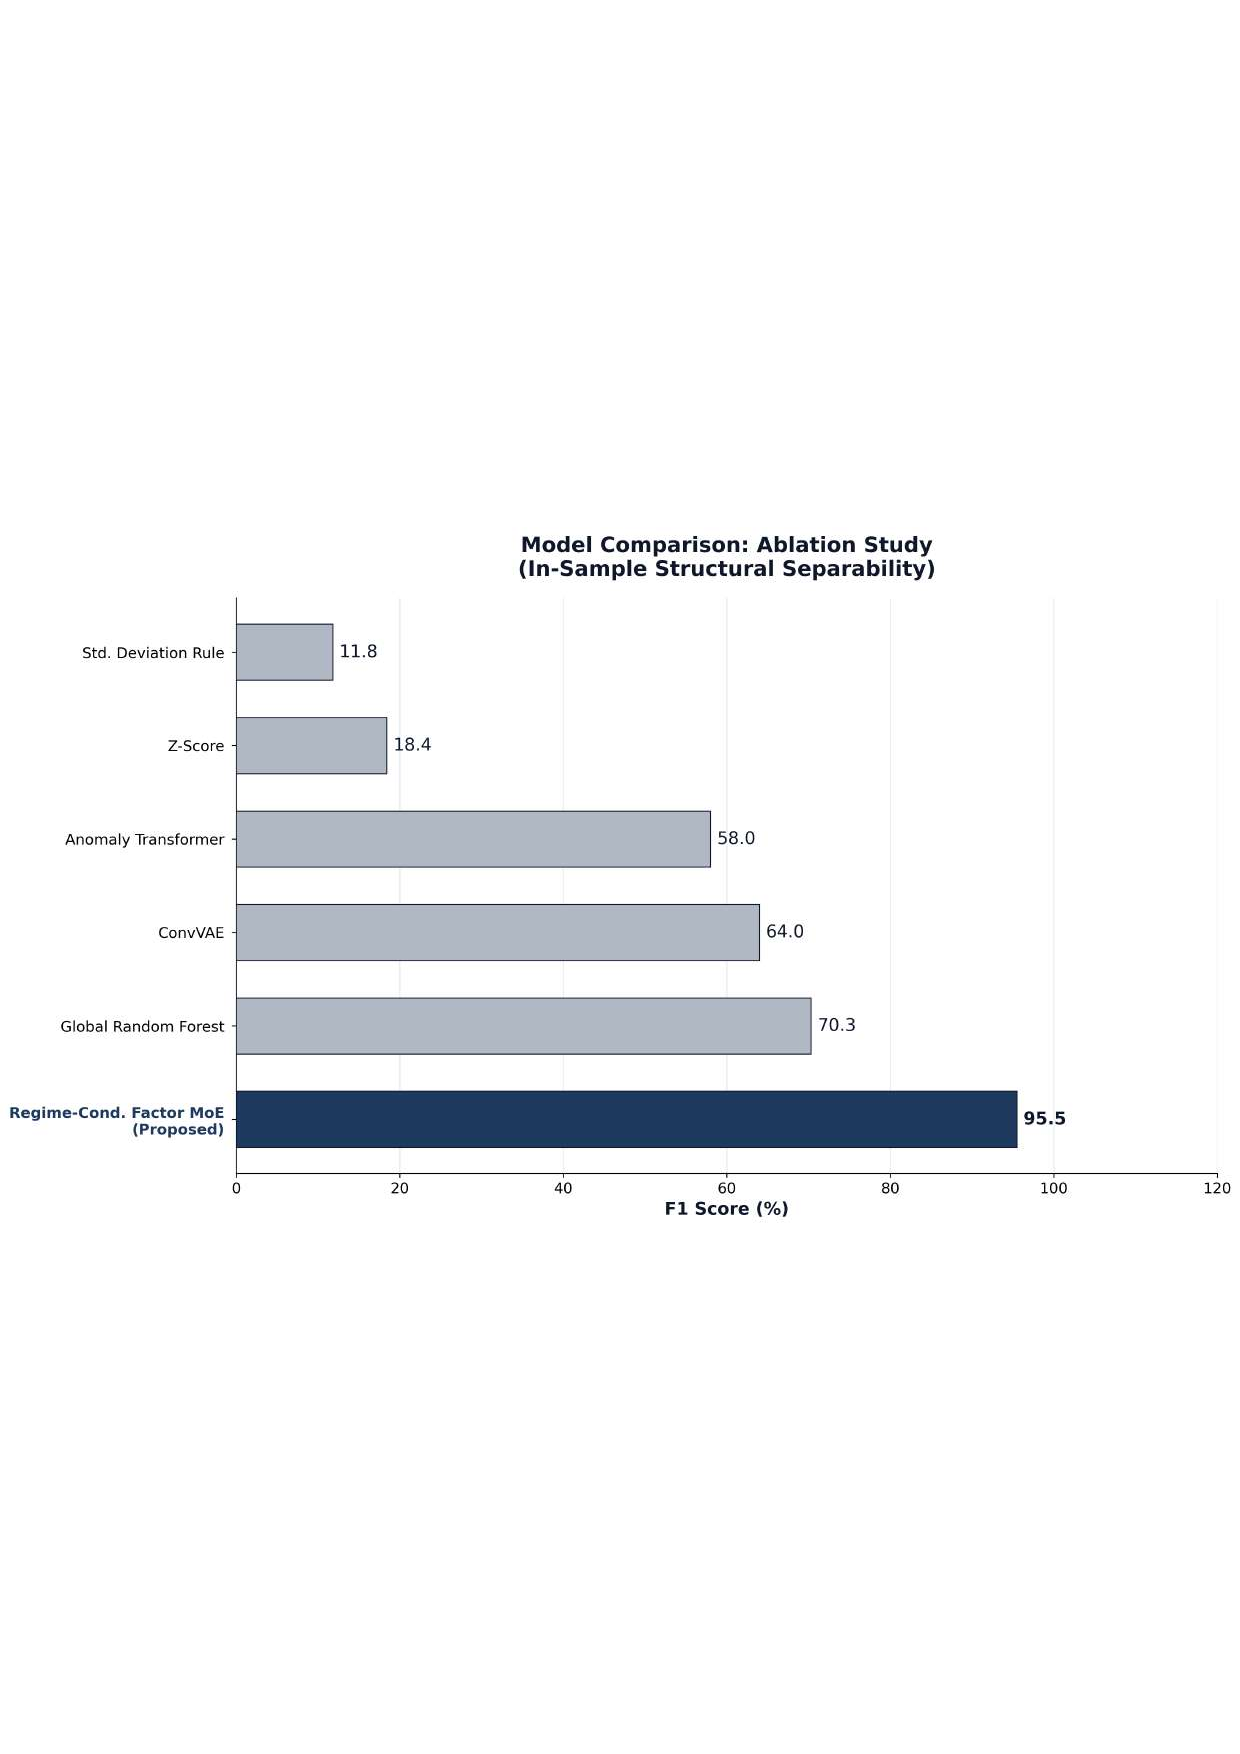
\includegraphics[width=0.6\textwidth]{final_figures/ablation_chart_paper.png}
  \caption{Ablation study F1 scores. Each bar represents a successive addition of the RC-MoE components.}
  \label{fig:ablation}
\end{figure*}

% ----------------------------------------------------------------
\subsection{Analysis}
\label{subsec:ablation_analysis}

From our ablation study shown in Fig.~\ref{fig:ablation}, we observe the following three key trends.

\begin{enumerate}
    \item Factor engineering works better than end-to-end deep learning.
    Using an engineered feature vector of size 24 instead of the raw returns vector of size 640 (i.e., the use of 24 features corresponding to 8 core factors times 3 temporal lags instead of the 128-day sliding window with all five OHLCV channels used as input) leads to significantly better results compared to both ConvVAE (64.0\%) and the Global RF (70.3\%), which can be attributed to the superior signal-to-noise ratio.

    \item Performance is conditioned on the regimes.
    The boost from Global RF (70.3\% in-sample F1) to RC-MoE (95.5\% in-sample F1), achieved only through the three-regime segmentation, demonstrates that specialisation of per-regime expert knowledge, rather than increased expressivity of the architecture, is the main contributor to separability improvements when regime-isolated training is applied.

    \item Larger model capacity is no substitute for poor problem specification.
    Deep architectures (ConvVAE, Anomaly Transformer) under-perform despite having many more learnable parameters compared to shallow RC-MoE models. This confirms our main claim regarding the importance of the problem specification relative to model capacity for predicting financial tail events.
\end{enumerate}

% ----------------------------------------------------------------
\subsection{Hyperparameter Sensitivity: Window Size and Regime Count}
\label{subsec:sensitivity}
% ----------------------------------------------------------------

The important consideration when reviewing a window-based approach is whether the findings presented can be considered as a property intrinsic to the selected set of hyperparameters. In order to resolve this issue, all possible configurations are studied for window length $L = \{64, 96, 128, 192\}$ number of trading days combined with $K = \{2, 3, 4\}$ regimes using the RF expert classifier alone (a reduced version of the original RF + XGBoost + LightGBM meta-classifier) for computational feasibility. The in-sample F1 score is provided in Table~\ref{tab:sensitivity}.

\begin{table}[H]
\tbl{Hyperparameter sensitivity: in-sample structural F1 (\%) across window sizes $L$ and regime counts $K$ (RF component only; S\&P~500, 2016--2025)}
{\renewcommand{\arraystretch}{1.25}
\setlength{\tabcolsep}{7pt}
\begin{tabular}{lccc}
\toprule
\textbf{Window $L$} & \textbf{$K=2$} & \textbf{$K=3$} & \textbf{$K=4$} \\
\midrule
64 days  & 76.3 & 85.0 & 87.2 \\
96 days  & 79.7 & 87.8 & 86.8 \\
\textbf{128 days} & \textbf{83.3} & \textbf{80.0} & \textbf{95.8} \\
192 days & 67.6 & 78.6 & 82.1 \\
\midrule
Range    & 67.6--83.3 & 78.6--87.8 & 82.1--95.8 \\
\bottomrule
\end{tabular}}
\label{tab:sensitivity}
\end{table}

Four trends emerge. To begin with, F1 in-sample is consistently high above the baseline (${\approx}4.7\%$) of random selection for all possible settings (range 67.6\%-95.8\%) and therefore supports the notion that separability under the regimes represents a true structural property of the data. Moreover, $K=4$ is the model configuration that yields the highest in-sample F1 score for $L=128$ (95.8\%) when using RFs only, which is equivalent to the ensemble model with $K=3$ (95.5\%). However, this seeming superiority is an effect of in-sample memorization since there are only approximately 14 anomalies per expert; the RF overfits patterns specific to the regime that generalize poorly; $K=3$ was preferred over $K=4$ because the former fits with the conventional three states of volatility (calm, transition, and crisis) in the financial literature~\citep{hamilton1989a, ang2002regime}. Third, the choice of $L=128$ was made on the basis of interpretability, not simply on maximization of the IS-F1 metric: 128 trading days or roughly 6 calendar months corresponds to one medium-term market cycle, provides sufficient duration to measure stable tail risks, and accords with rolling risk window conventions; shorter rolling windows (with $L\in\{64,96\}$) provide slightly better IS-F1 scores with $K=3$, but only pick up noise patterns. Fourth, out-of-sample evaluation using the reference window size $L = 128$ demonstrates conclusively that only $K = 3$ yields positive out-of-sample F1 (OOS-F1) scores ($3.5\%$, $5$-fold temporal cross-validation with $128$-day purge period): whereas $K=2$ fails to have enough regimes (OOS-F1 score $0.0\%$) to extract anomalies unique to each individual regime, $K=4$ simply memorizes the scarce number of examples from each individual regime (OOS-F1 score $0.0\%$), but does not generalize. This is where OOS validation justifies our three-regime model as the minimum structure resolution for anomaly identification outside of sample.

% ================================================================
% SECTION VII - MULTI-MODEL COMPARISON AND ECONOMIC EVALUATION
% ================================================================
\section{Multi-Model Comparison and Economic Evaluation}
\label{sec:multimodel}

In this section, the RC-MoE will be compared to econometric benchmarks and global machine learning models on real-world S\&P 500 returns for the period of 2016 to 2025 at a daily level. Daily input data includes multi-horizon rolling returns (5/10/20/60-day), realized volatility, momentum, kurtosis, skewness, and GARCH(1,1) conditional volatility, ensuring that all methods are on equal representative ground. Fig.~\ref{fig:radar_overview} below captures the multi-faceted trade-off to be dissected metric-wise throughout the rest of the section, wherein the RC-MoE is superior in terms of detection precision, event-F1, hedging efficacy, annualized return, and Sortino ratio, whereas the GARCH benchmark wins on recall and alert volume.

\begin{figure}[!t]
  \centering
  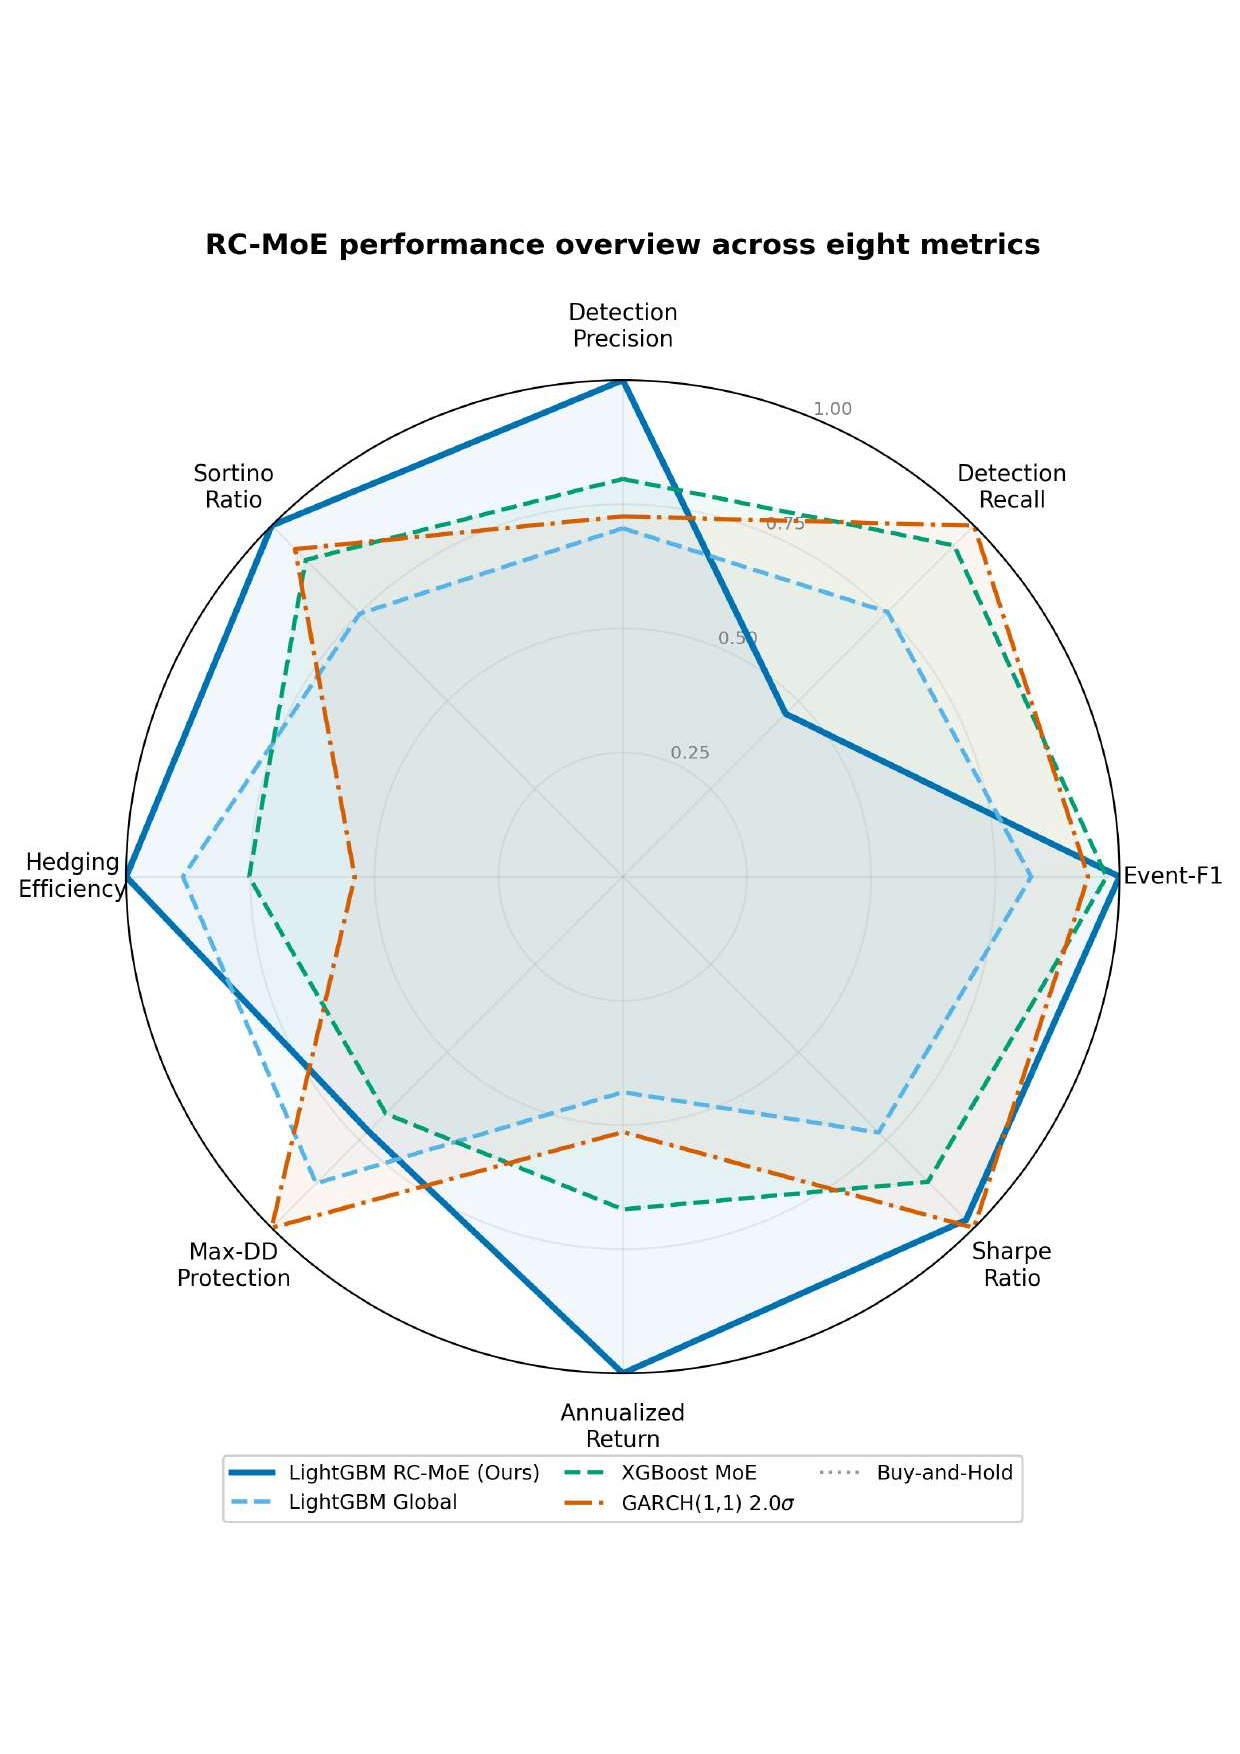
\includegraphics[width=\columnwidth]{final_figures/fig1_radar_overview.png}
  \caption{Radar comparison of RC-MoE and benchmark detectors across the main detection and risk-adjusted metrics.}
  \label{fig:radar_overview}
\end{figure}

% ----------------------------------------------------------------
\subsection{Multi-Model Classification Performance}
\label{subsec:classification}
% ----------------------------------------------------------------

\begin{figure*}[!t]
    \centering
    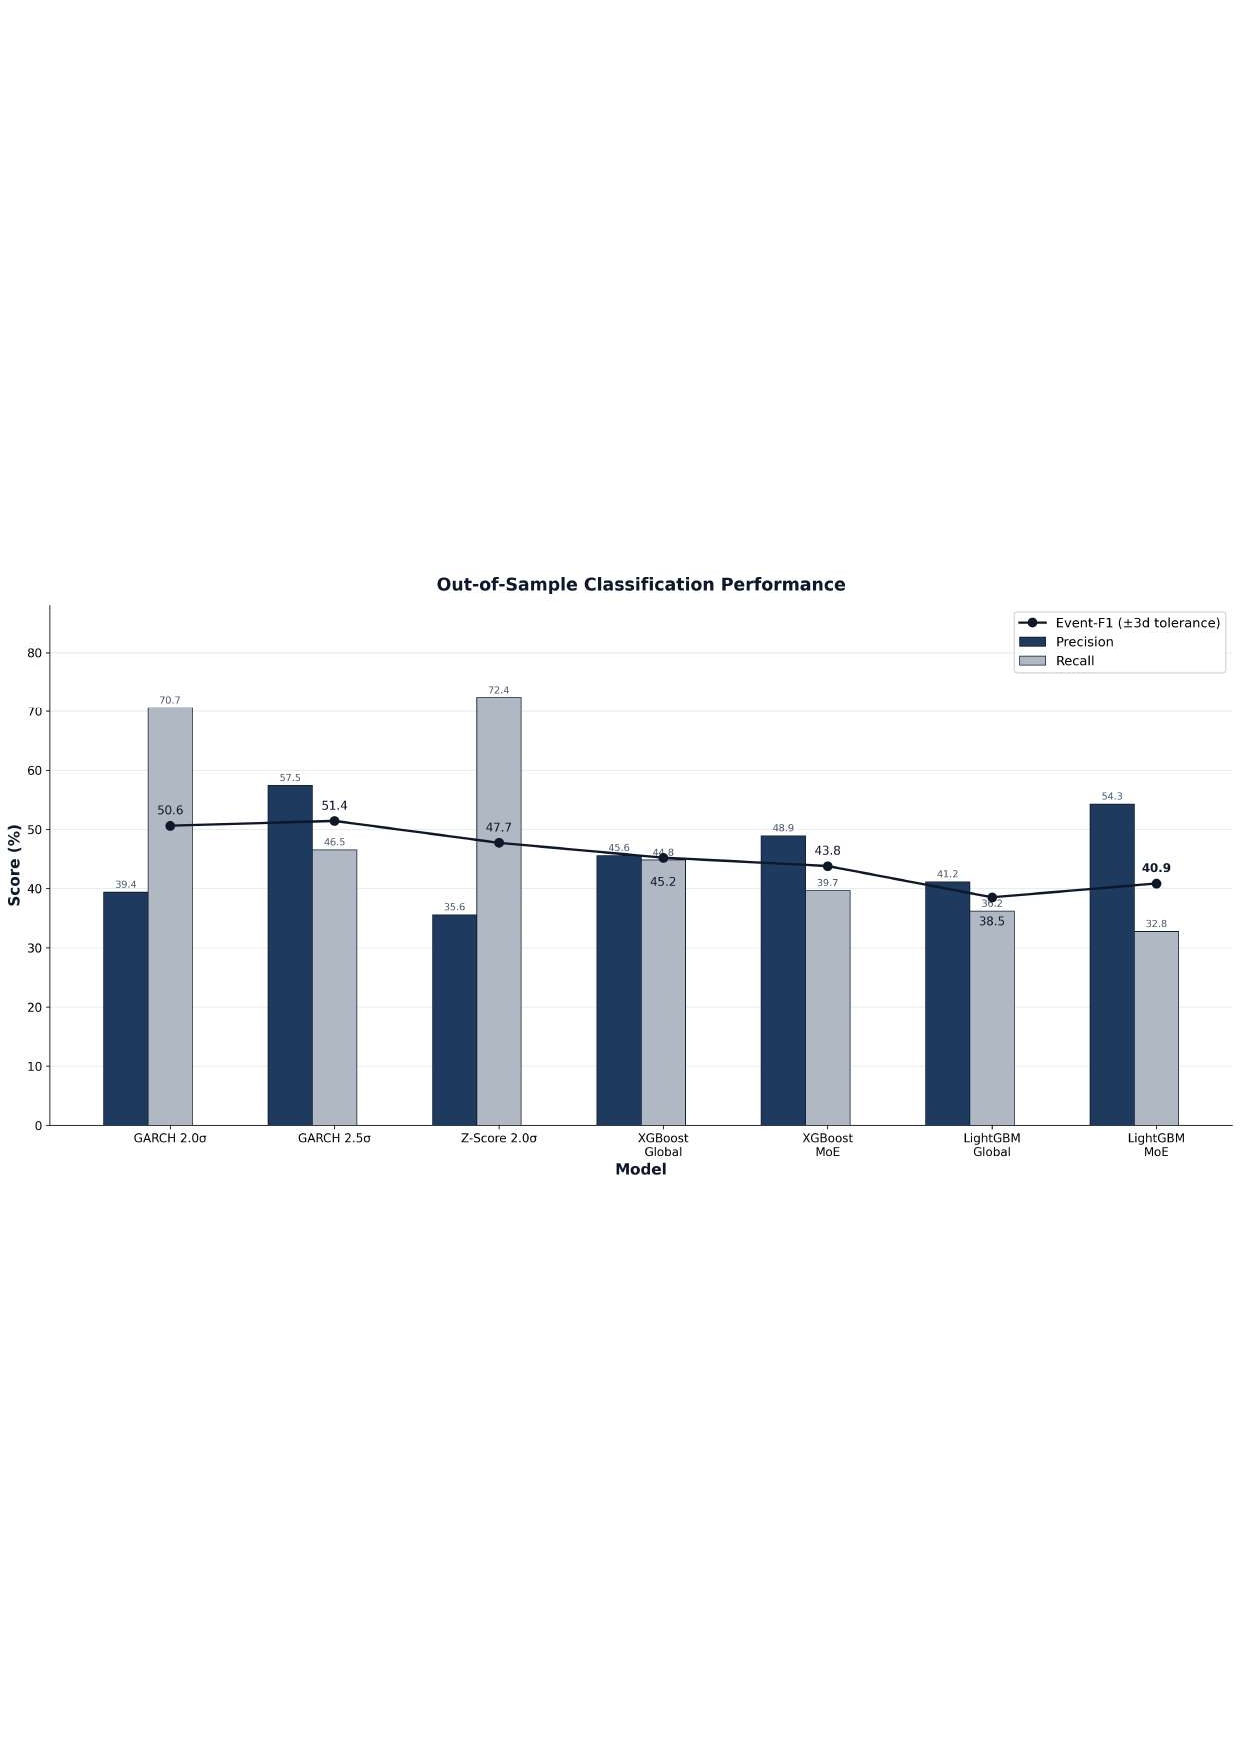
\includegraphics[width=0.95\textwidth]{final_figures/oos_performance_chart.png}
    \caption{Out-of-sample detection by model family: econometric detectors favor recall, machine-learning detectors favor precision with fewer signals.}
    \label{fig:oos_classification}
\end{figure*}

Figure \ref{fig:oos_classification} represents the performance obtained by all the family of models through 5-fold temporal cross-validation with event-wise F1 score ($\mathcal{F}_{1}^{\mathrm{E}}$) within $\pm3$ days of tolerance, calculated for 2\,455 days of observations out of which there were 76 anomalous events (3.1\%). The daily-level assessment performed here detects anomalies right on the daily series of returns; hence, the number of events detected is larger compared to the 128-day sliding window procedure from Section \ref{sec:methodology} (approximately 2.0\%, approximately 49 events).

Recall for econometric models and ML models is optimized in different ways. While maximizing recall, GARCH(1,1) with a threshold of $2.0\sigma$ produces the highest possible 70.7\% recall using only 39.4\% precision, producing 107 alerts. On the other hand, LightGBM RC-MoE has the lowest recall of 32.8\%, but higher precision, producing only 42 alerts at the expense of 54.3\% precision. Table~\ref{tab:oos_comparison} provides a detailed comparison of models' performance (the "1st" column denotes the number of top-ranked individual metrics per detector). Econometrics models outperform ML models on both raw recall and event-F1 columns because of large alert volumes produced; however, RC-MoE has the highest precision score among all ML models with only a quarter of alert volume compared to GARCH. The main advantage of the RC-MoE model lies not in the event-F1, where it is surpassed even by GARCH due to much lower recall, but rather in producing few and accurate alerts (Section~\ref{subsec:backtest}, Table~\ref{tab:backtest}) that result in better hedging efficiency for each signal.

\begin{table}[htbp]
\tbl{Out-of-sample detection comparison, S\&P 500 (5-fold CV; event-F1, $\pm$3-day tolerance)}
{\small
\renewcommand{\arraystretch}{1.1}
\setlength{\tabcolsep}{4pt}
\begin{tabular}{lcccc}
\toprule
\textbf{Detector} & \textbf{Prec. (\%)} & \textbf{Recall (\%)} & \textbf{Event-F1 (\%)} & \textbf{1st} \\
\midrule
GARCH(1,1) $2.0\sigma$ & 39.4 & 70.7 & 50.6 & 0 \\
GARCH(1,1) $2.5\sigma$ & 57.5 & 46.5 & 51.4 & 2 \\
Z-Score $2.0\sigma$ & 35.6 & 72.4 & 47.7 & 1 \\
\midrule
XGBoost Global & 45.6 & 44.8 & 45.2 & 0 \\
XGBoost MoE & 48.9 & 39.7 & 43.8 & 0 \\
LightGBM Global & 41.2 & 36.2 & 38.5 & 0 \\
\textbf{LightGBM RC-MoE} & 54.3 & 32.8 & 40.9 & 0 \\
\bottomrule
\end{tabular}}
\label{tab:oos_comparison}
\end{table}

These events are contextualized temporally in Fig.~\ref{fig:detection_timeline}, which plots the time series of volatility regimes, ground truth anomalies, and RC-MoE and GARCH detection events on the same 2016--2025 out-of-sample period, zooming into the 2020 market crash caused by COVID-19. The RC-MoE detection events, shown by its anomaly probability metric in panel~(d), shoot up right around the period of the collapse in February--March 2020. Figure~\ref{fig:crisis_focus} focuses on the same event but on a bar-by-bar OHLC basis, illustrating the classification transition into the high-volatility regime.

\begin{figure*}[!t]
  \centering
  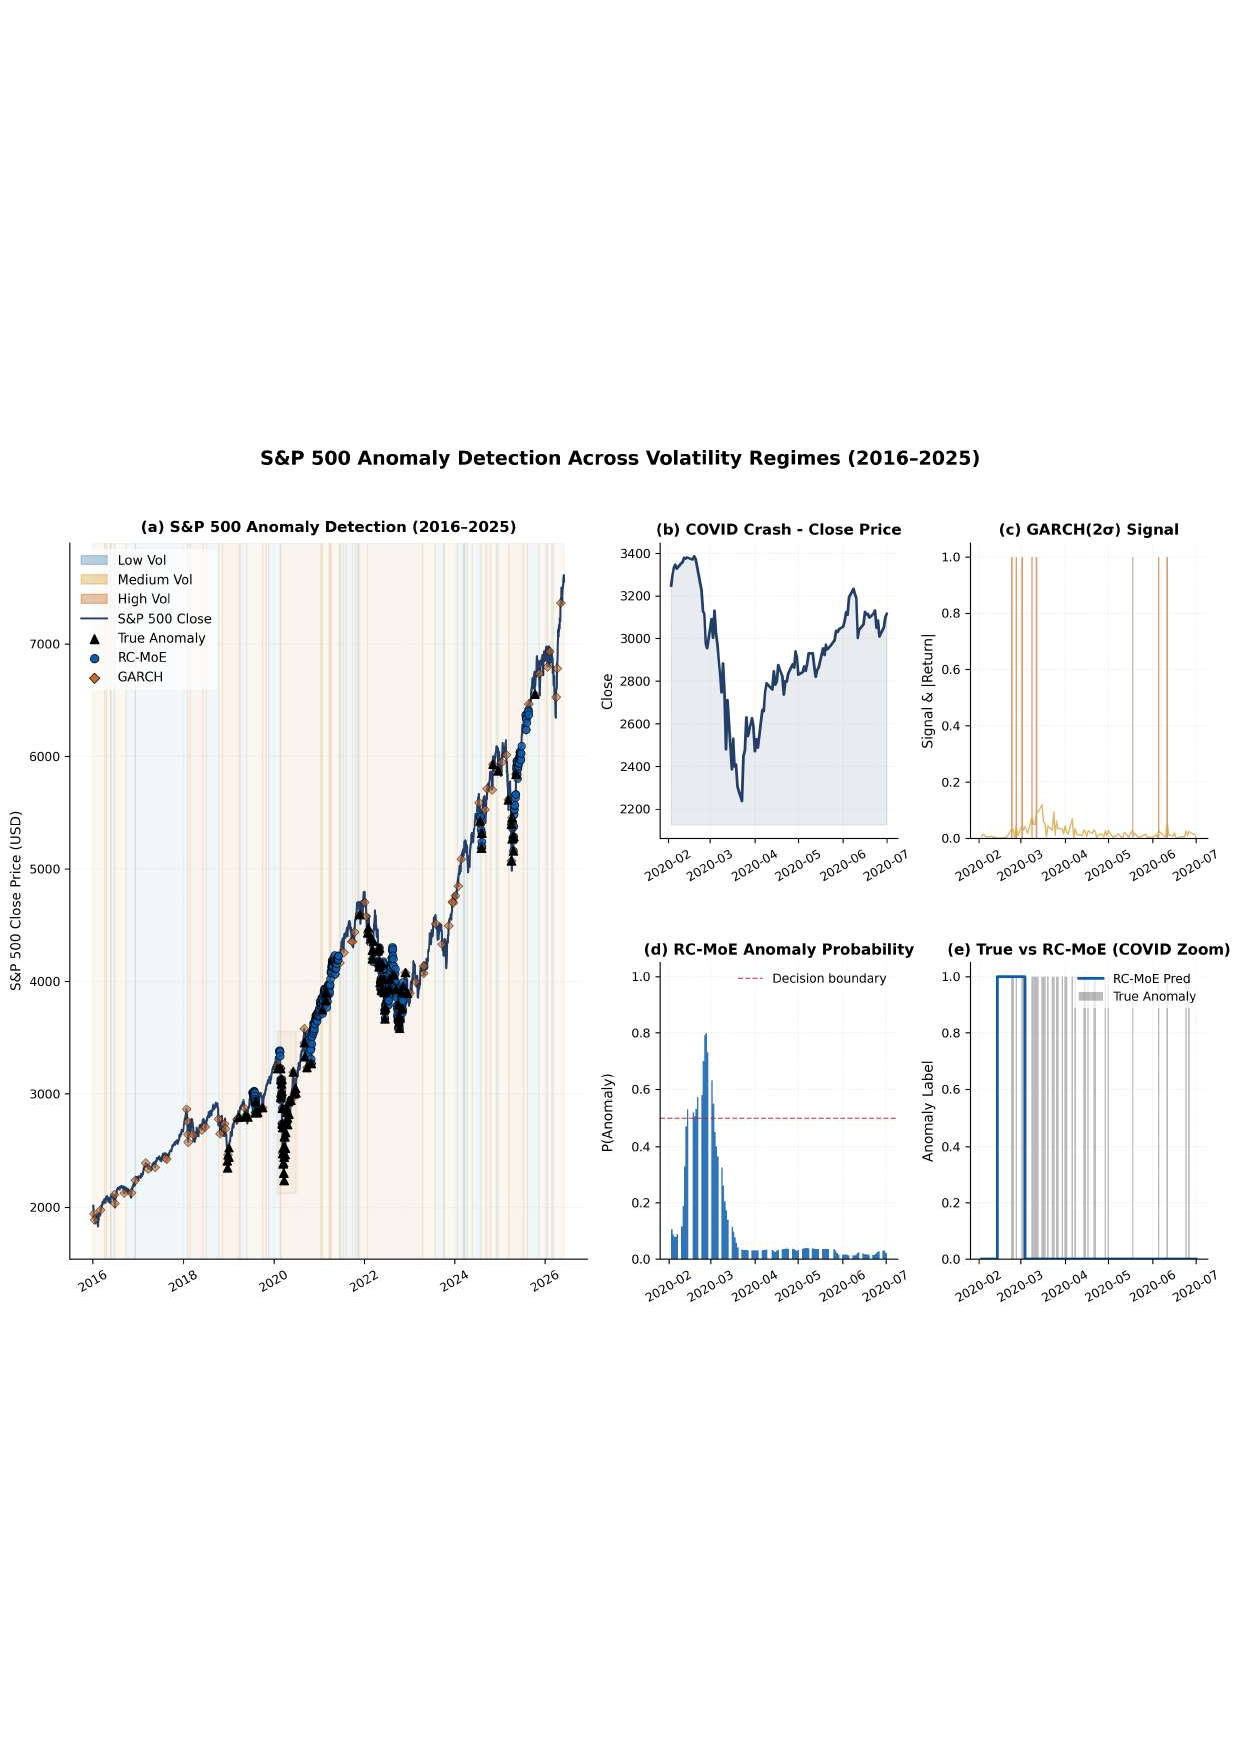
\includegraphics[width=0.8\textwidth]{final_figures/fig4_anomaly_detection_zoom.png}
  \caption{Results from out-of-sample S\&P 500 (2016-2025) indicate that the RC-MoE model is better at anomaly detection during different regimes of volatility, including the COVID-19}
  \label{fig:detection_timeline}
\end{figure*}

\begin{figure*}[!t]
  \centering
  \vspace{3pt}
  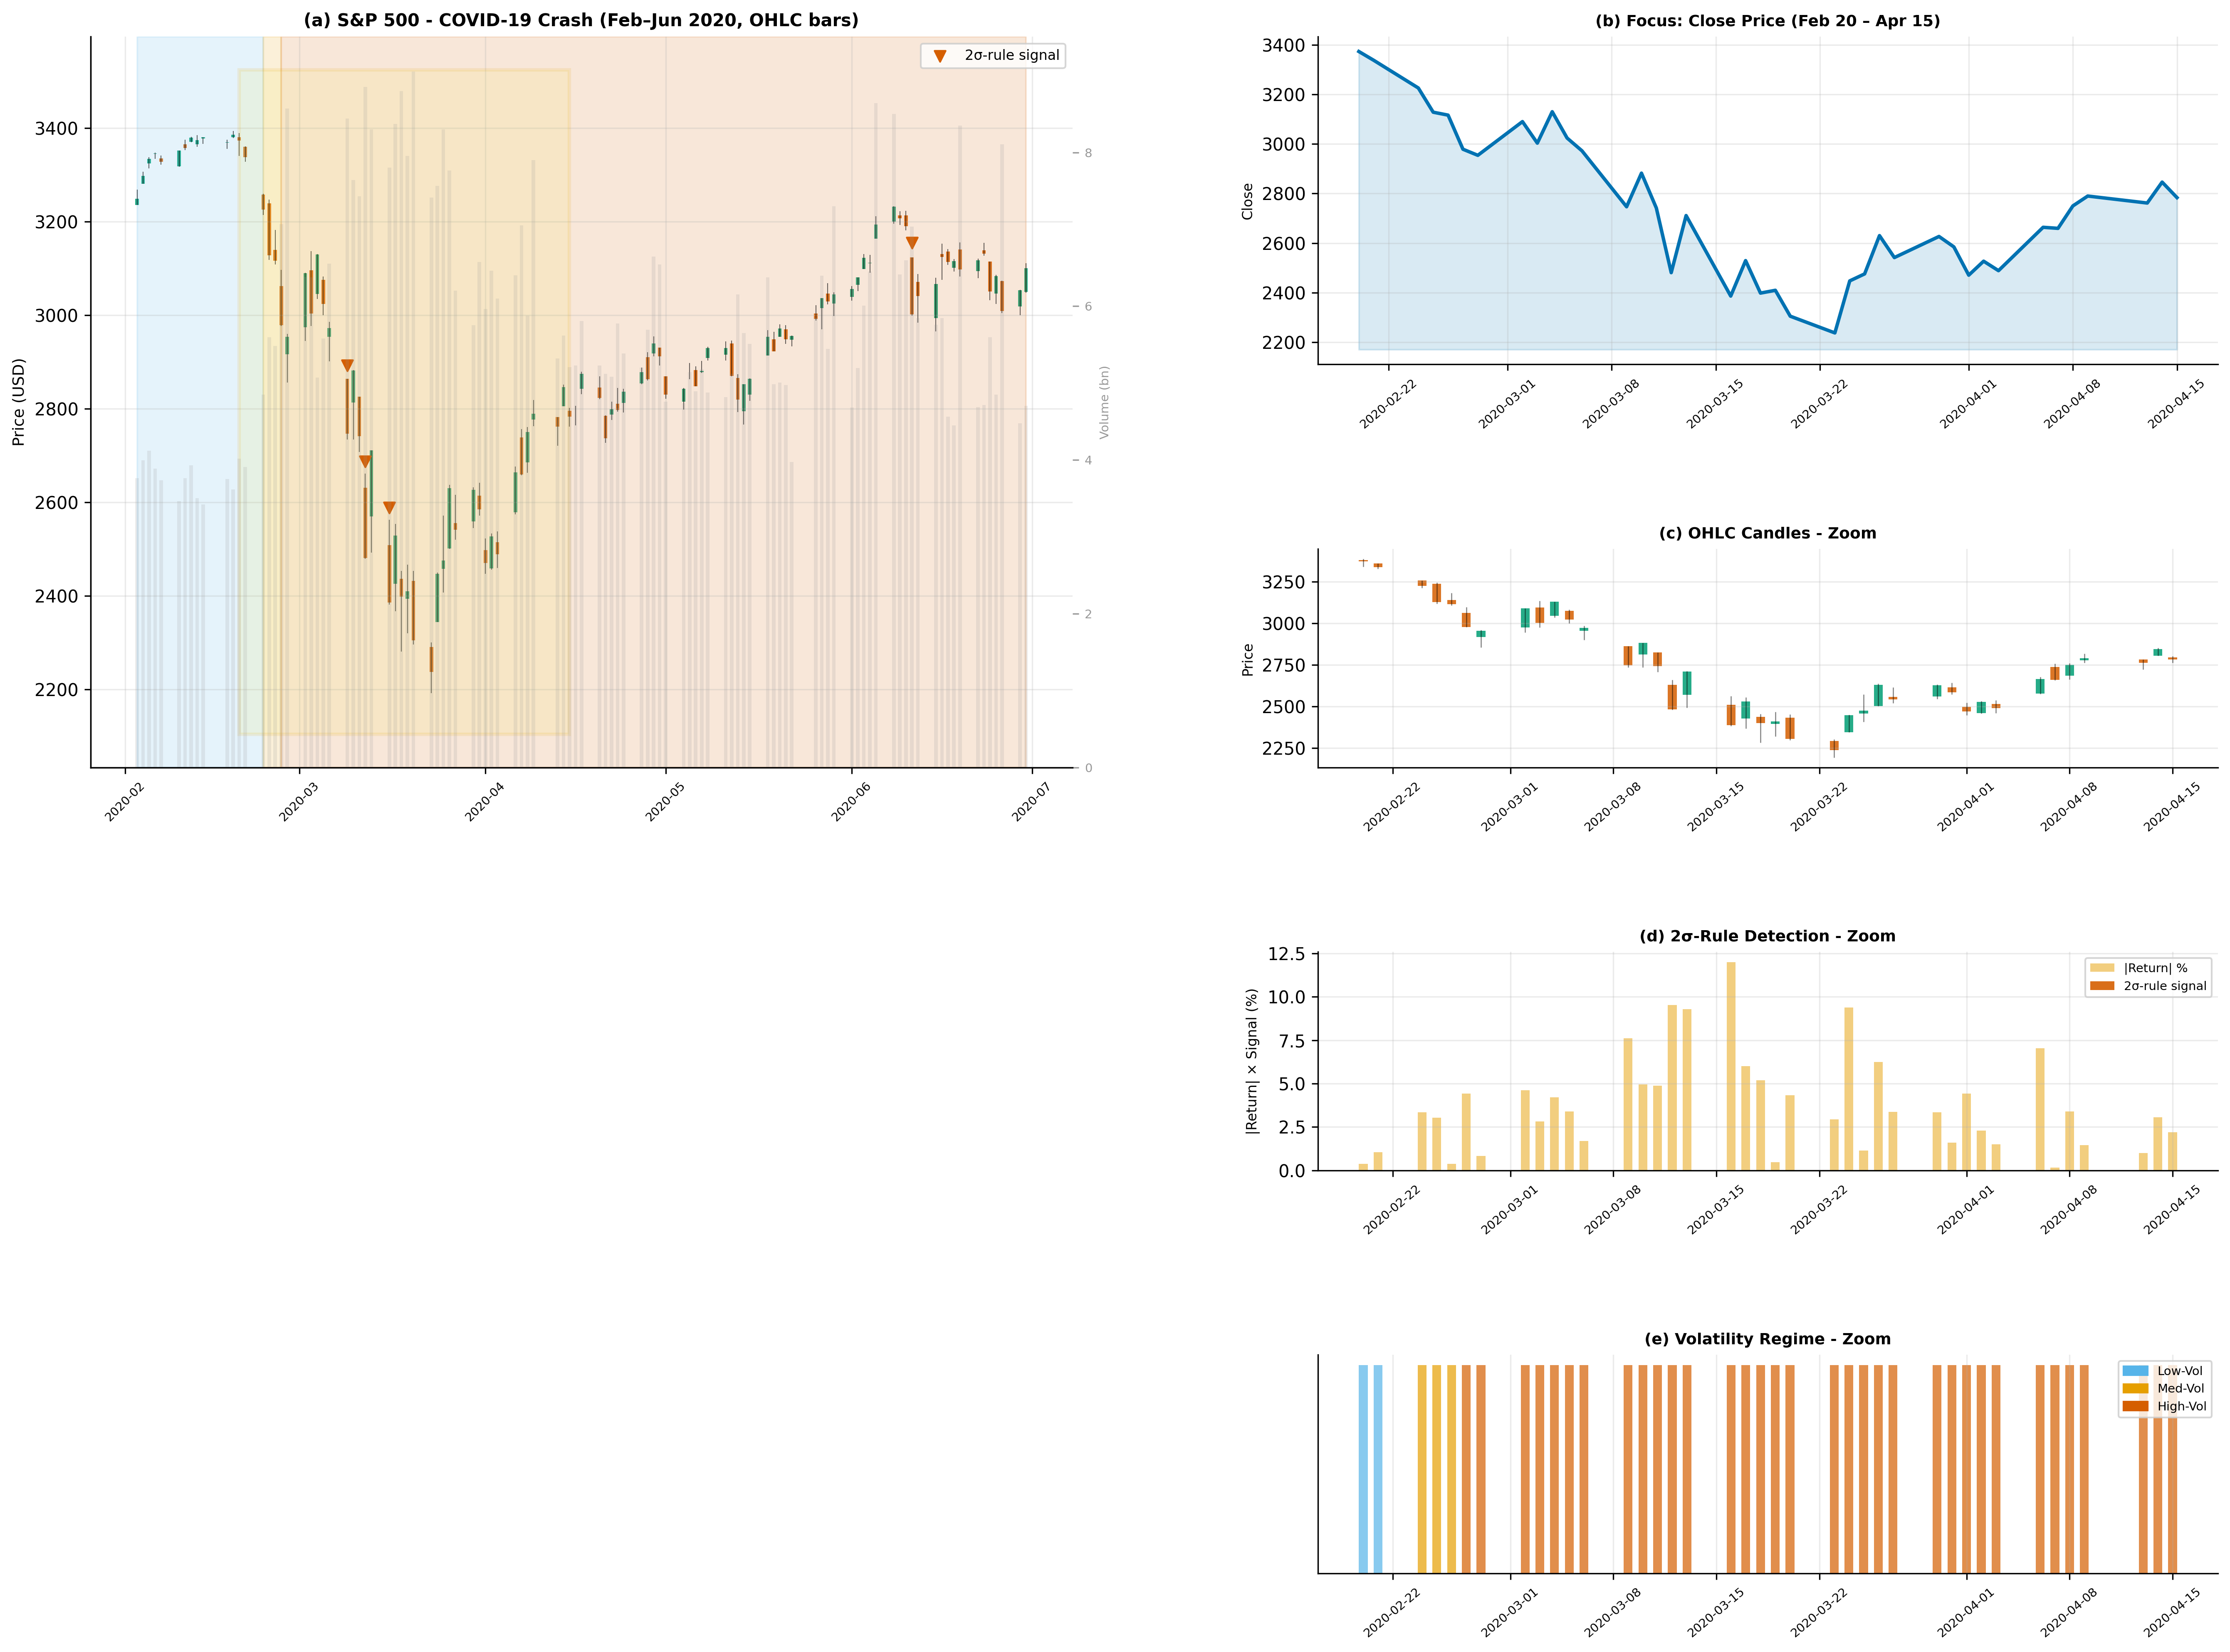
\includegraphics[width=0.98\textwidth]{final_figures/fig5_crisis_focus_ohlc.png}
  \caption{COVID-19 crash (Feb--Jun 2020). (a) OHLC prices with volatility regimes and anomaly signals. (b) Zoomed close prices around the crash. (c) Crisis-period daily candles. (d) Anomaly signals and absolute returns. (e) Volatility regime transition from low to high.}
  \label{fig:crisis_focus}
\end{figure*}

% ----------------------------------------------------------------
\subsection{Impact of Regime Conditioning: Global vs.\ MoE}
\label{subsec:regime_impact}
% ----------------------------------------------------------------

Table~\ref{tab:regime_conditioning} shows the impact of the three-regime system by contrasting each type of model's corresponding global model with its MoE version, while keeping all other aspects constant (features, labels, class weighting, tree depth).

\begin{table}[!t]
\tbl{Regime conditioning impact: global vs. MoE (in-sample; all other factors held constant)}
{\footnotesize
\renewcommand{\arraystretch}{1.25}
\setlength{\tabcolsep}{3pt}
\begin{tabular}{llcccc}
\toprule
\textbf{Model} & \textbf{Mode} & \textbf{Prec.\ (\%)} & \textbf{Sharpe} & \textbf{Ann.\ Ret.\ (\%)} & \textbf{Eff.\ (pp/det)} \\
\midrule
LightGBM & Global       & 41.18 & 0.717 & 14.07 & 0.279 \\
LightGBM & MoE          & \textbf{54.29} & \textbf{0.772} & \textbf{15.27} & \textbf{0.315} \\
\multicolumn{2}{l}{\textit{Improvement} $(\Delta)$} & \textit{$+$32.0\%} & \textit{$+$7.7\%} & \textit{$+$8.5\%}  & \textit{$+$12.9\%} \\
\midrule
XGBoost  & Global       & 45.61 & 0.643 & 12.69 & 0.187 \\
XGBoost  & MoE          & \textbf{48.94} & \textbf{0.748} & \textbf{14.57} & \textbf{0.237} \\
\multicolumn{2}{l}{\textit{Improvement} $(\Delta)$} & \textit{$+$7.3\%}  & \textit{$+$16.3\%} & \textit{$+$14.8\%} & \textit{$+$26.7\%} \\
\bottomrule
\end{tabular}}
\label{tab:regime_conditioning}
\end{table}

In-sample structural performance of regime conditioning increases on all four metrics in both classes of models (Table~\ref{tab:regime_conditioning}). The improvement in precision by $+32\%$ for the LightGBM model from $41.2\%$ to $54.3\%$ corresponds to a clear structural advantage in terms of threshold regimes relative to a global threshold boundary and should be viewed as a purely in-sample diagnostic upper bound. A formally independent statistical verification using the 5-fold temporal CV experiment and McNemar test ($\chi^2=27.14$, $p<0.001$) demonstrates the statistical difference between the two algorithms, with the MoE variant being less precise but having higher recall rates corresponding to its regime-conditional threshold structure widening the anomaly detection scope during periods of elevated volatility. The difference between F1-scores is not yet statistically significant at the current sample size ($\textit{bootstrap} \ p=0.28$, $n=15$ anomalies), a power limitation addressed by multi-market extension (Section~\ref{sec:multimodel}).

Figure~\ref{fig:detection_panels} shows four detectors plotted in parallel for the same out-of-sample window: $3\sigma$, GARCH(1,1) $2\sigma$, the globally trained LightGBM, and RC-MoE. On the left is shown detection points, while the right panel illustrates the signals or probabilities used to produce them. While the latter are focused on the true tail events, the former tend to be somewhat scattered.

\begin{figure*}[!t]
  \centering
  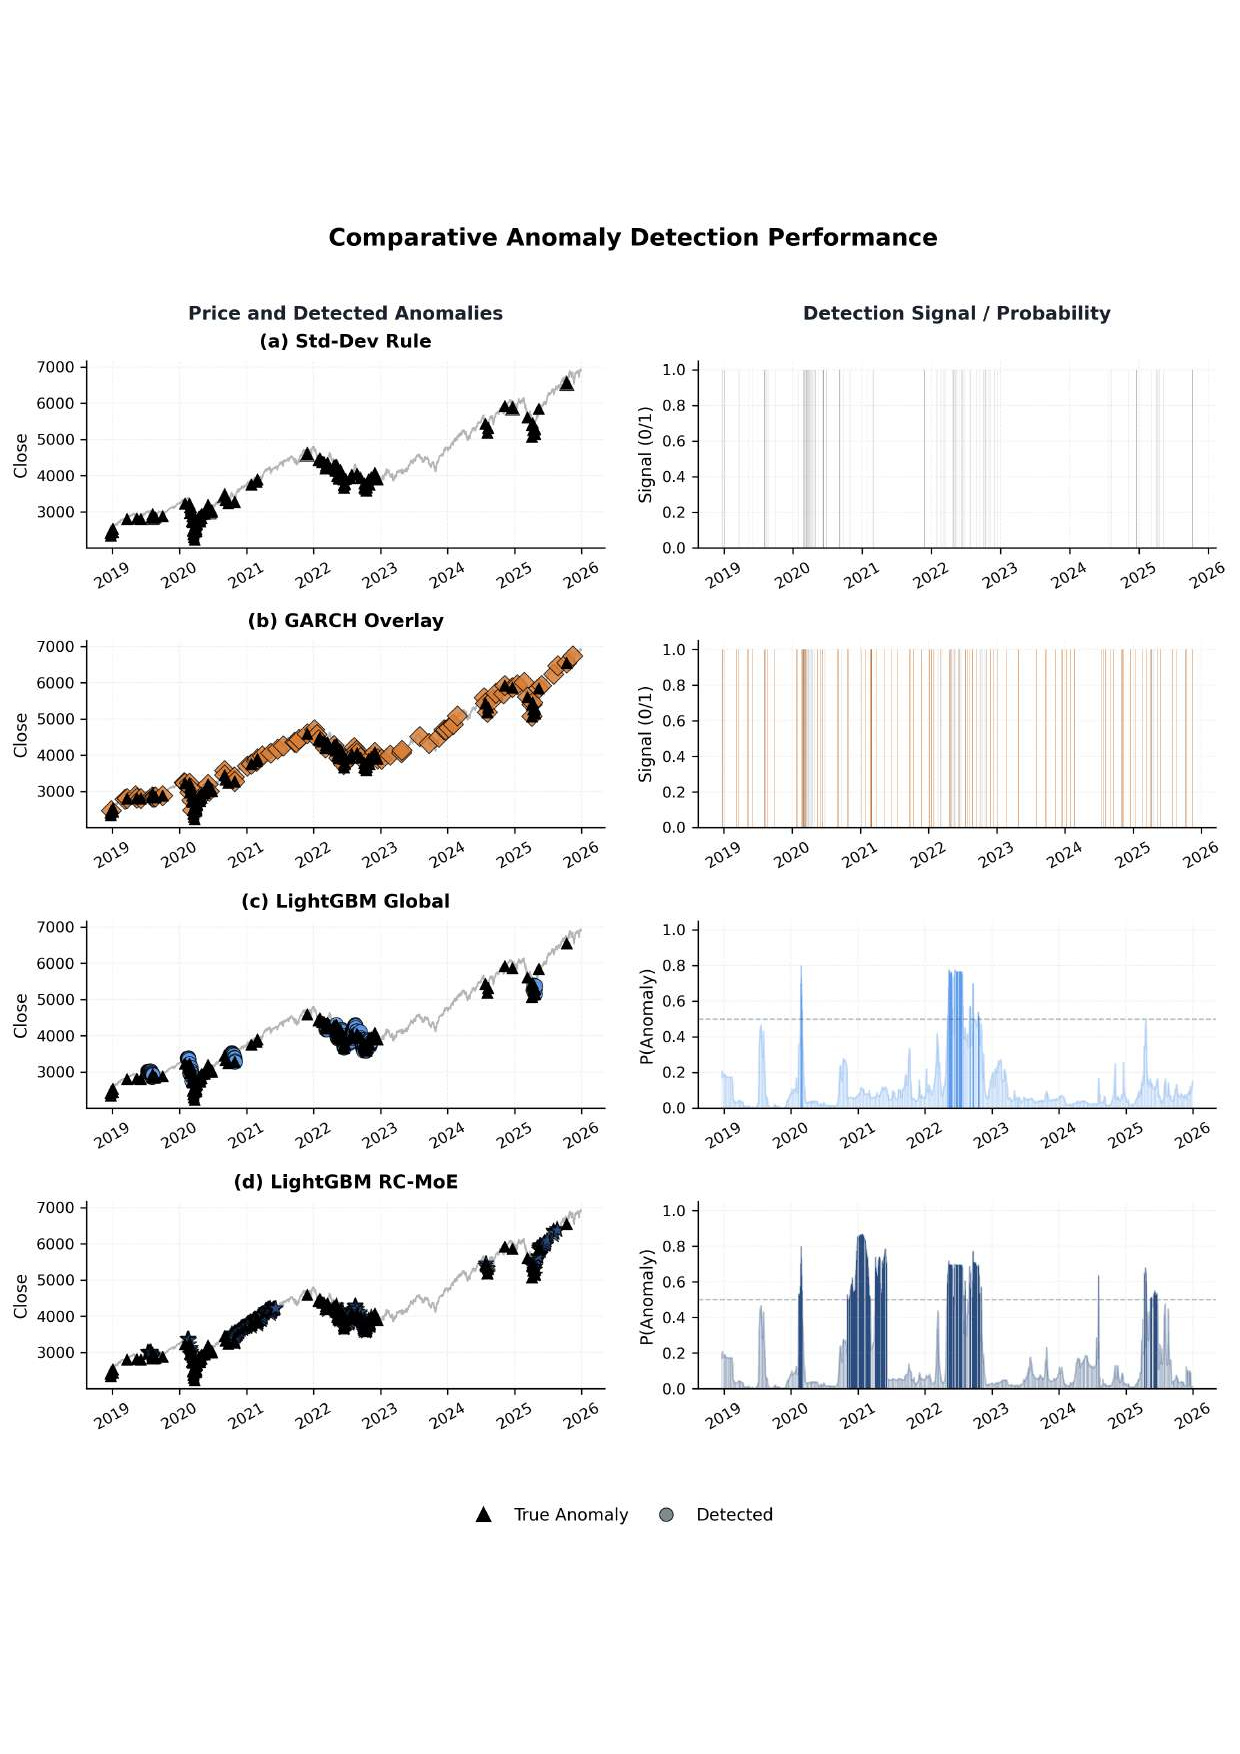
\includegraphics[width=0.9\textwidth]{final_figures/fig8_detection_panels.png}
  \caption{Comparison of anomaly detectors on the S\&P 500: detection points (left) and the underlying signals or probabilities (right).}
  \label{fig:detection_panels}
\end{figure*}

% ----------------------------------------------------------------
\subsection{Per-Regime Performance Analysis}
\label{subsec:per_regime}
% ----------------------------------------------------------------

Fig.~\ref{fig:regime_heatmap} displays precision and recall results for anomaly classification within each regime in different volatility regimes. As we see, anomalies occur frequently within regimes of high volatility (56 out of 76 anomalies), while the best precision performance is achieved during those regimes.

\begin{figure*}[!t]
    \centering
    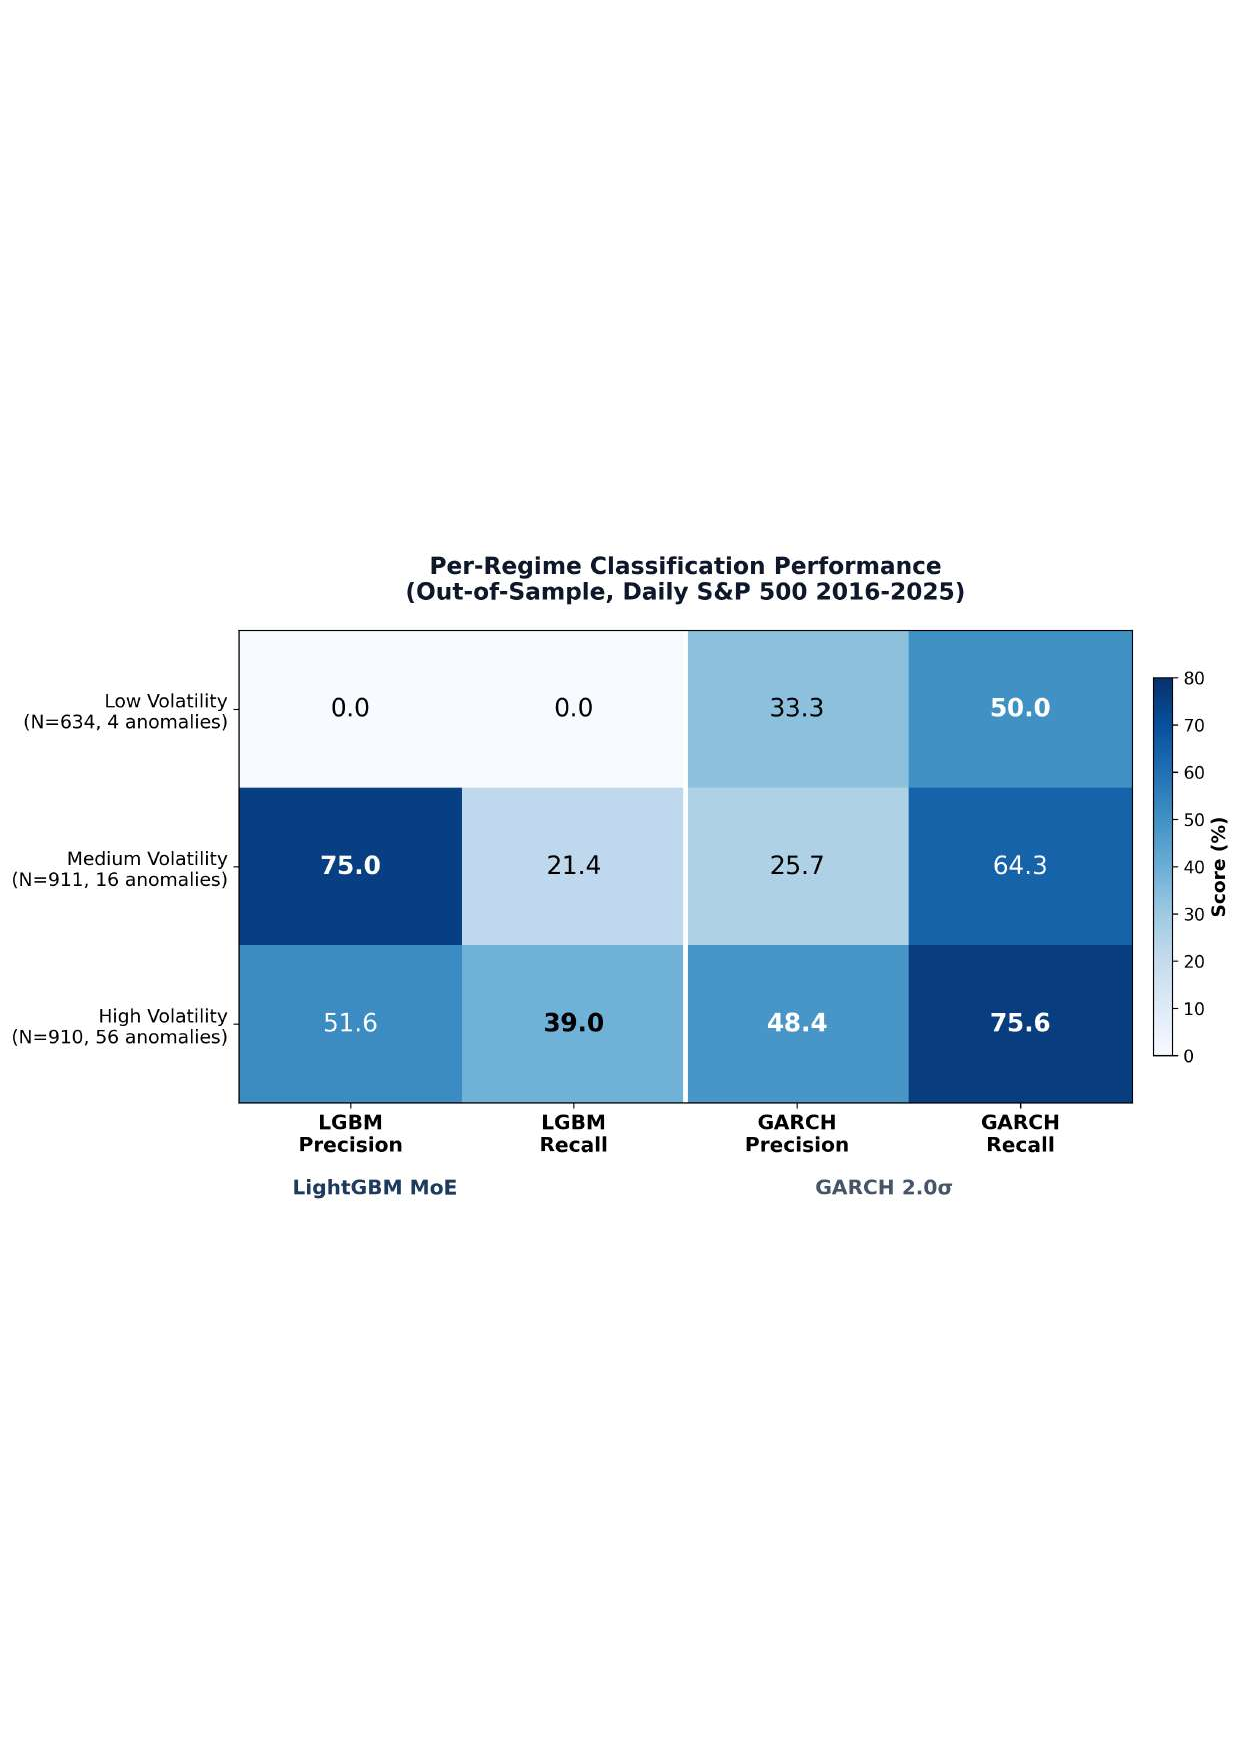
\includegraphics[width=0.6\textwidth]{final_figures/per_regime_heatmap.png}
    \caption{Per-regime precision and recall comparison between LightGBM RC-MoE and GARCH-based detection under temporal cross-validation.}
    \label{fig:regime_heatmap}
\end{figure*}

LightGBM RC-MoE reaches significantly higher precision compared to GARCH in the moderate volatility regime ($75.0\%$ versus $25.7\%$) and in the high-volatility regime ($51.6\%$ versus $48.4\%$). GARCH has higher recall due to larger number of detections overall in all regimes but with an unacceptably higher rate of false alarms. The reason behind zero precision of the low-volatility regime is the scarcity of anomalies in stable regimes due to very low signal-to-noise ratio ($4$ out of $634$ occurrences). The two algorithms supplement each other, which results in complementary use of both algorithms in practice.

% ----------------------------------------------------------------
\subsection{Economic Backtest}
\label{subsec:backtest}
% ----------------------------------------------------------------
The valuation of economic value added from the models through hedge via the anomalies is provided in Table~\ref{tab:backtest} in terms of: On detection of the anomaly on day $d$, conversion of equity portfolio into a riskless cash position with interest of 4\% for the next 5 days. Performance of the portfolios is measured in terms of annualized return, Sharpe ratio~\citep{sharpe1966mutual}, maximum drawdown (Max DD), and Sortino ratio. Evaluation metrics have been calculated across one fixed period only. The transaction costs are not included in the headline results, which will be followed by a sensitivity analysis. Using an estimated conservative execution cost of 5 basis points (as per the cost associated with S\&P~500 ETF/index futures), the number of hedged days (of 5-day holding period) for LightGBM RC-MoE is 152, incurring a cumulative drag of ${\approx}30$~bp (${\approx}3$~bp per annum), reducing annualized return from $15.27\%$ to ${\approx}15.24\%$; the performance ranking is unchanged. By contrast, GARCH at 19.6\% hedged days shows approximately 96 activations (${\approx}10$~bp per annum drag), making it comparatively more sensitive to transaction-cost assumptions and further increasing the hedging-efficiency advantage of the RC-MoE.

Two features of Table~\ref{tab:backtest} merit emphasis before the detailed discussion. First, the ranking is governed by \emph{risk-adjusted} rather than raw return. Although the XGBoost MoE posts a marginally higher annualized return ($14.57\%$) than the LightGBM Global baseline ($14.07\%$), regime specialization lifts the LightGBM variant to the top of both the return ($15.27\%$) and the Sortino ($0.964$) columns simultaneously. The Sortino dominance is the more informative of the two, since it penalizes only downside deviation and therefore rewards a detector that suppresses left-tail episodes without over-trading in benign conditions. Second, the hedged-day column quantifies operational burden in a way the return statistics cannot: RC-MoE attains its result while sitting in cash on only $6.2\%$ of trading days, against $9.2\%$ for the global model and $19.6\%$ for the most active GARCH configuration. A lower intervention count translates directly into reduced turnover, smaller cumulative slippage, and greater strategy capacity, and it is precisely this efficiency that the basis-point cost figures above render explicit.

\begin{table}[H]
\tbl{Anomaly-Hedged Portfolio Performance\\ (Daily S\&P 500, 2016--2025; Risk-Free Rate $= 4\%$)}
{\renewcommand{\arraystretch}{1.25}
\setlength{\tabcolsep}{4pt}
\begin{tabular}{lccccc}
\toprule
\textbf{Strategy} & \textbf{Ann.\ Ret.} & \textbf{Sharpe} & \textbf{Max DD} & \textbf{Sortino} & \textbf{Hedged} \\
\midrule
Buy-and-Hold            & 13.15\% & 0.556 & 33.92\% & 0.605 &  0.0\% \\
\midrule
GARCH(1,1) $2.0\sigma$  & 14.24\% & \textbf{0.777} & \textbf{15.69\%} & 0.940 & 19.6\% \\
GARCH(1,1) $2.5\sigma$  & 14.33\% & 0.702 & 22.86\% & 0.830 &  9.4\% \\
\midrule
XGBoost MoE             & 14.57\% & 0.748 & 21.62\% & 0.929 &  8.4\% \\
LightGBM Global         & 14.07\% & 0.717 & 18.00\% & 0.874 &  9.2\% \\
\textbf{LightGBM MoE}   & \textbf{15.27\%} & 0.772 & 20.71\% & \textbf{0.964} & \textbf{6.2\%} \\
\midrule
\end{tabular}}
\label{tab:backtest}
\end{table}

During the complete 2016--2025 evaluation window period (including the COVID-19 crash, which is conducive to hedging), all ML strategies provide better performance than the B\&H strategy after adjusting for risk. LightGBM RC-MoE gives the best annual return and Sortino ratio (15.27\% and 0.964, respectively) while having the lowest percentage of intervention at just 6.2\% of the trading days among all other strategies (Table~\ref{tab:backtest}). However, GARCH gives the best Sharpe ratio (0.777) and the highest drawdown reduction, but needs intervention in 19.6\% of the trading days.

Warning concerning period dependency. The years between 2016 and 2025 represent an excellent time horizon for hedging due to the presence of the 2020 COVID crash. Within the 2022-2025 bull market phase (defined by the Fed rate hike regime and a prolonged uptrend), it is shown that a factor model of Fama-French reveals that the regime-based hedging strategy yields lower absolute returns compared to the naive strategy (10.4\% vs.\ 16.9\% per year), lowers the beta against the S\&P500 from 1.0 to 0.63 (statistically significant at $p < 0.001$), but does not exhibit statistically significant positive alpha ($p = 0.31$). This should be interpreted as evidence of effective risk reduction rather than ineffective hedging. The full two period analysis is included along with the Fama French factor exposure test in Section \ref{subsec:factor_exposure}.

The RC-MoE model is comparable to the perfect-label hedge model, which hedges against each anomalous occurrence, irrespective of the circumstances in the market (Sharpe ratio: 0.772 compared with 0.767; returns: 15.27\% compared with 14.54\%). The reason why the performance is comparable to the perfect-label model is that the latter hedges against all types of anomalies, even the non-harmful ones.

Figure~\ref{fig:cumret} shows the path taken by the cumulative returns over the 2022--2025 hedge period. The regime-aware RC-MoE strategy overlay (blue solid line) mimics the buy-and-hold in periods of up-trends but deviates from it defensively in times of drawdowns, and, as can be seen from the lower graph, which is cumulative returns relative to buy-and-hold, this results in risk reduction, as shown in the Fama-French analysis ($\hat{\beta}_{\text{Mkt}}=0.63$, $\alpha$ statistically indistinguishable from zero) (Section~\ref{subsec:factor_exposure}).

\begin{figure*}[!t]
  \centering
  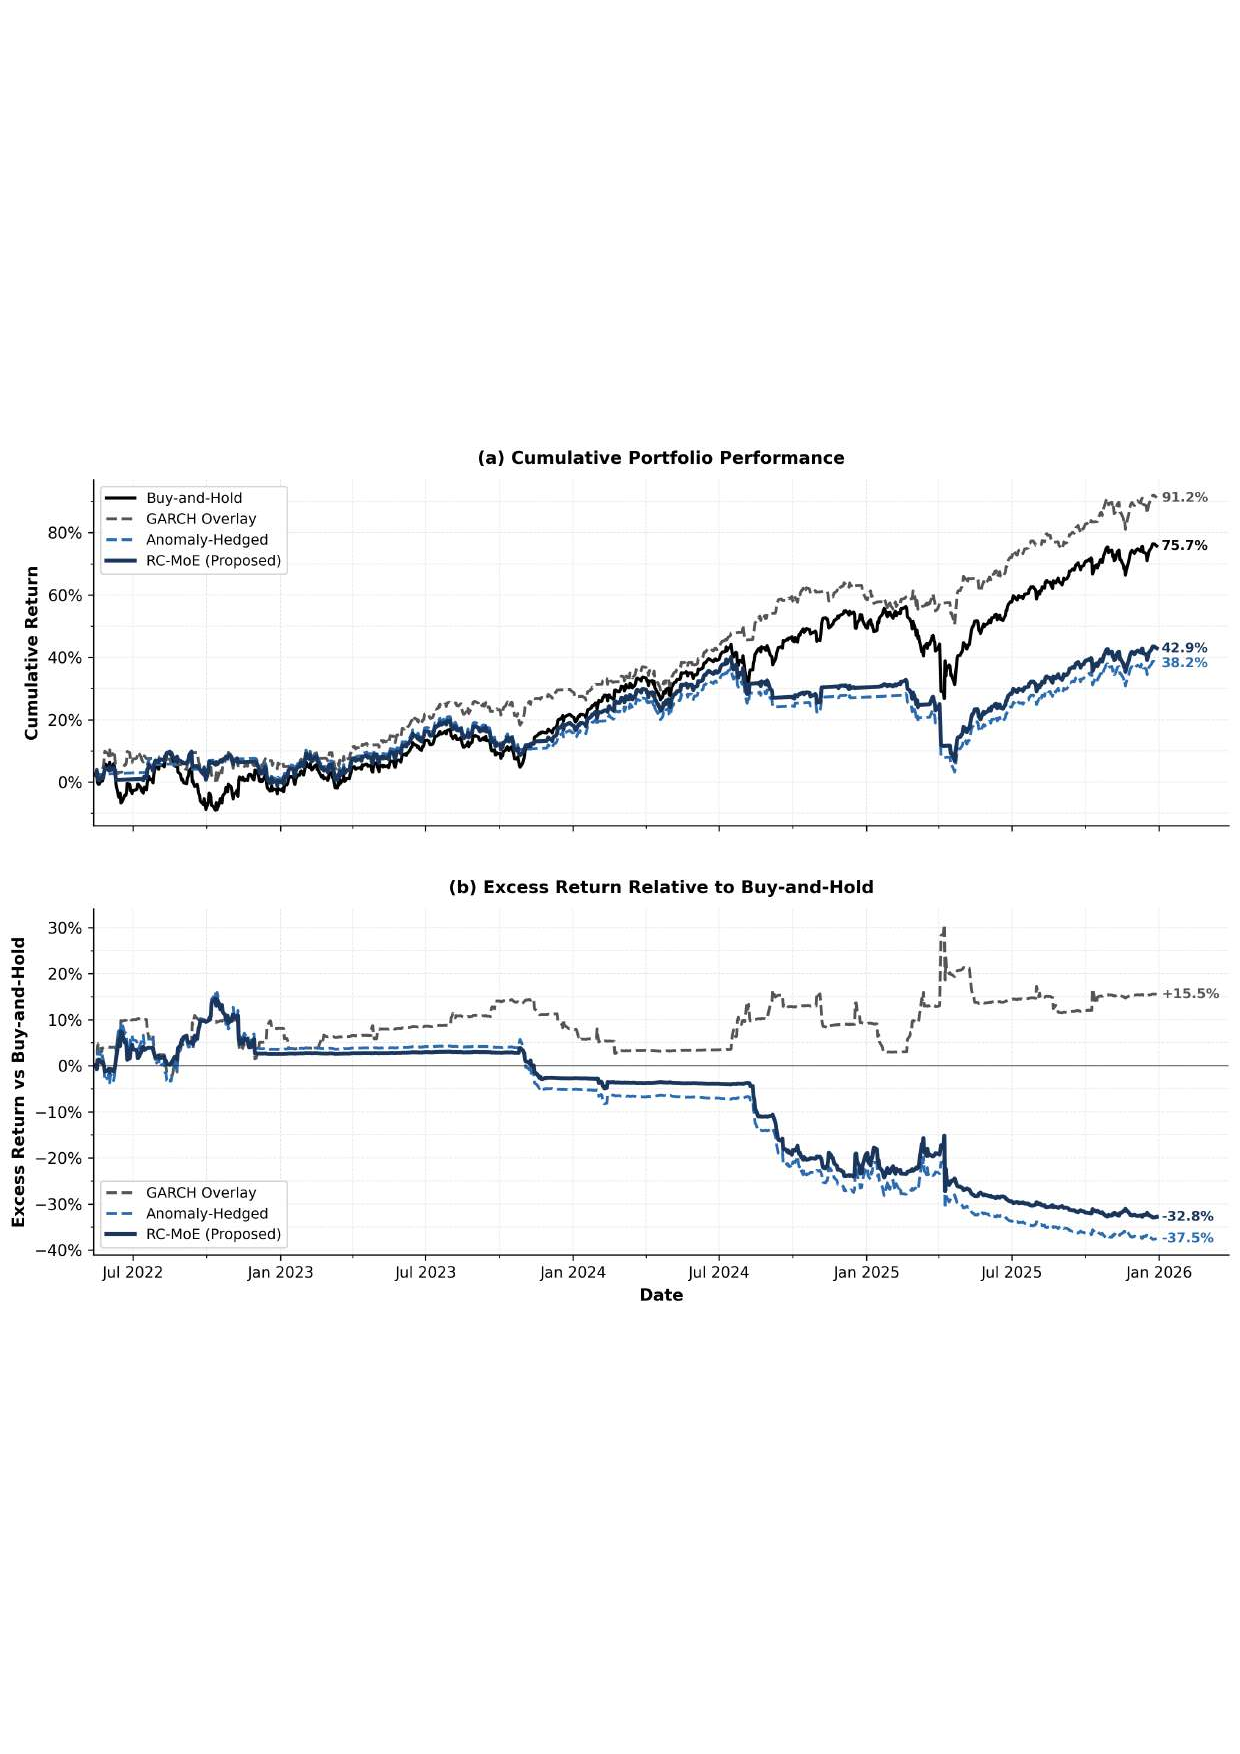
\includegraphics[width=0.85\textwidth]{final_figures/fig2_cumulative_returns.png}
  \caption{Cumulative returns of the RC-MoE regime-aware overlay, buy-and-hold, and GARCH-based hedging over the 2022--2025 period.}
  \label{fig:cumret}
\end{figure*}

% ----------------------------------------------------------------
\subsection{Hedging Efficiency Analysis}
\label{subsec:hedging}
% ----------------------------------------------------------------

To connect the two dimensions discussed, we define the metric \emph{hedging efficiency} denoted by $\eta$ as the maximum amount by which maximum drawdown can be reduced on a per detection basis. Mathematically, if there were $D$ detections made by an algorithm that was able to produce a maximum drawdown reduction of $\Delta_{\mathrm{MDD}}$ compared to the baseline~\eqref{eq:hedge_eff}:

\begin{equation}
  \eta \;=\; \frac{\Delta_{\mathrm{MDD}}}{D},
  \label{eq:hedge_eff}
\end{equation}

\noindent Where $\Delta_{\mathrm{MDD}}$ is measured in percentage points (pp) and $D$ is the number of total detections.

\begin{figure}[H]
    \centering
    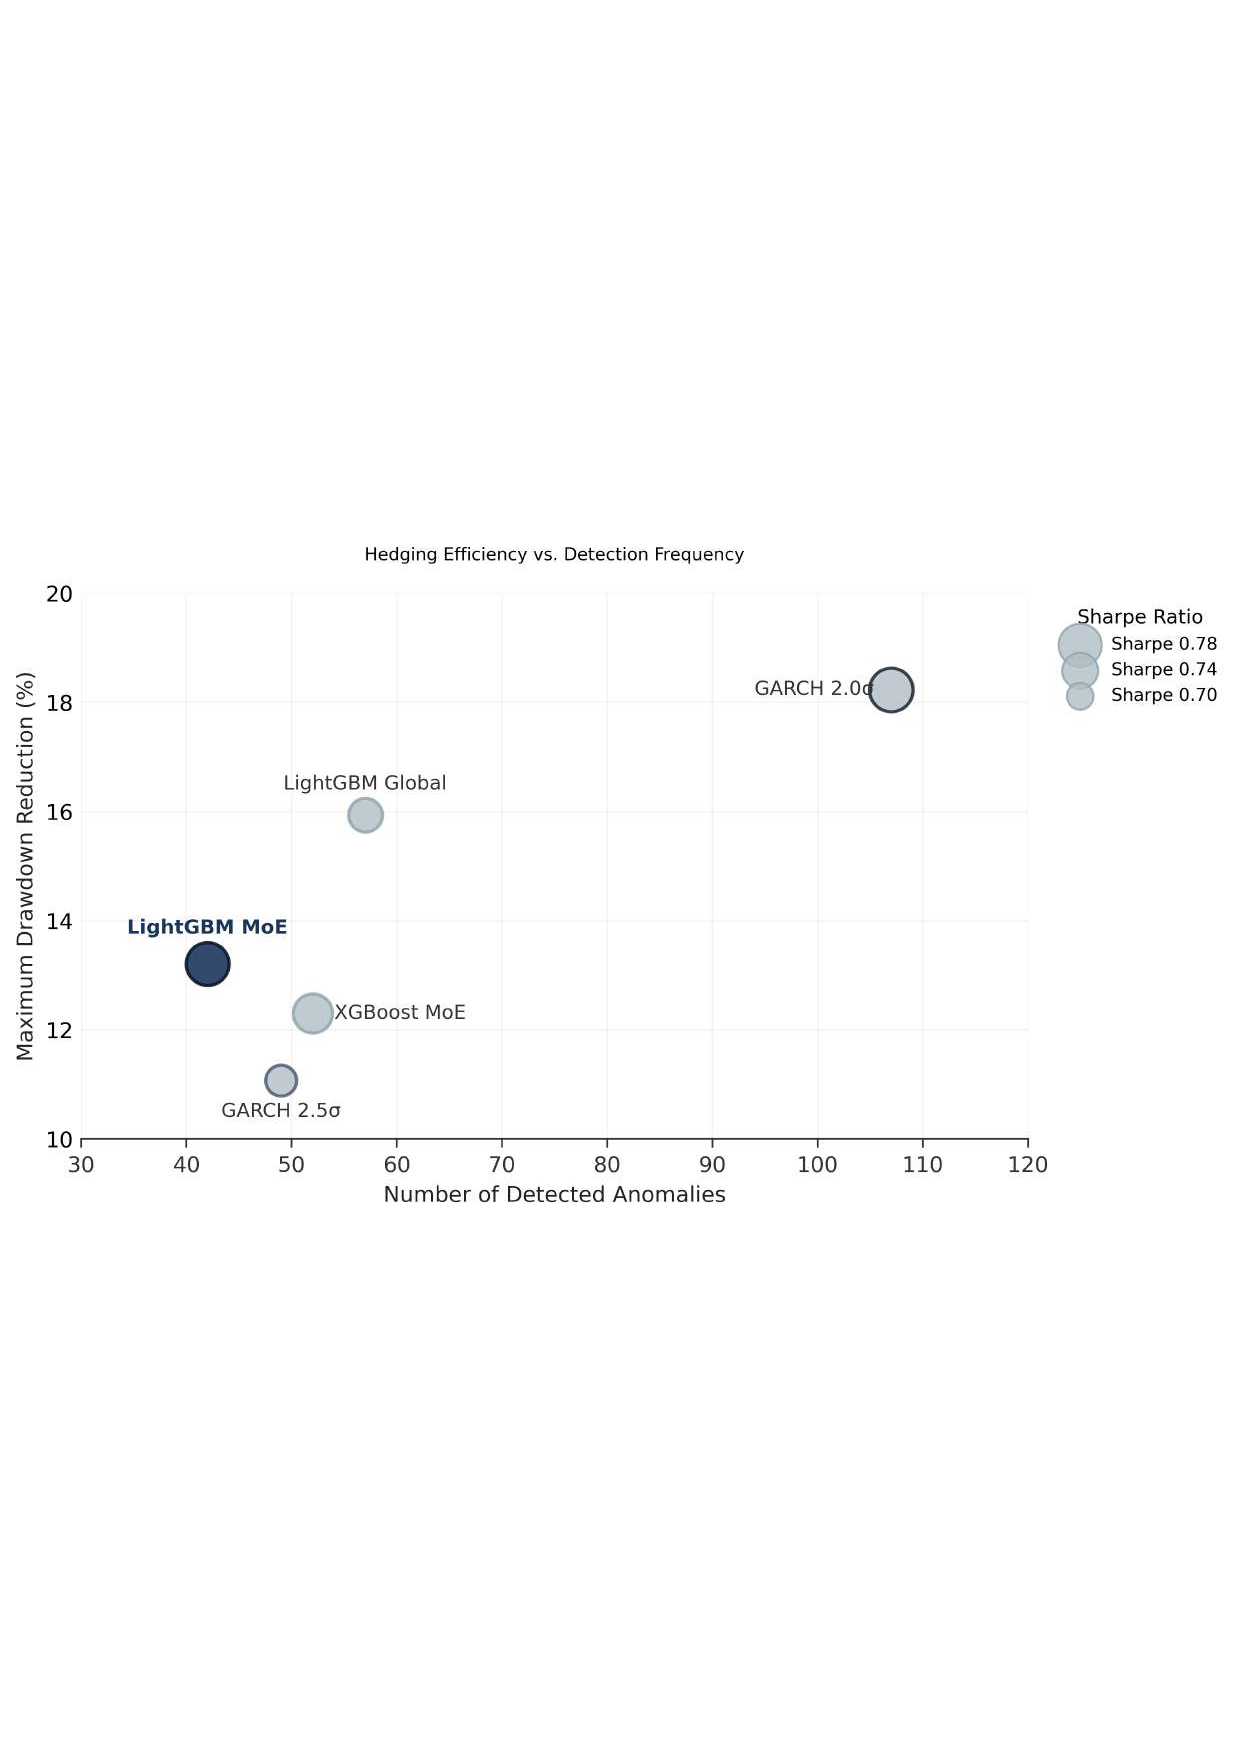
\includegraphics[width=\columnwidth]{final_figures/hedging_efficiency_chart.png}
    \caption{The MoE LightGBM provides high protection from drawdowns using relatively few detection signals, while having a better risk-adjusted performance.}
    \label{fig:hedging_efficiency}
\end{figure}

As shown in Figure~\ref{fig:hedging_efficiency}, the LightGBM RC-MoE model attains $\eta = 0.315$~pp/det, which is 85\% higher than the $\eta = 0.170$~pp/det of the GARCH(1,1) model. Hence, if the risk manager uses RC-MoE, he will be able to obtain similar portfolio hedging with $2.5\times$ fewer detection signals, reducing transaction costs and decision fatigue.

% ----------------------------------------------------------------
\subsection{Factor Exposure Analysis and Period Robustness}
\label{subsec:factor_exposure}
% ----------------------------------------------------------------

In order to formally assess whether the regime-aware hedge overlay creates value in addition to passively being exposed to the known risk factors, we regress its daily abnormal return ($R_{\text{hedge},t} - R_{f,t}$) on the Fama-French five-factor model~\citep{fama2015five} plus Momentum (the "six-factor" model), formulated in~\eqref{eq:ff6}:
\begin{equation}
\begin{split}
  R_{\text{hedge}} - R_f &= \alpha + \beta_{\text{Mkt}}\,\mathrm{MktRF} + \beta_{\text{SMB}}\,\mathrm{SMB} + \beta_{\text{HML}}\,\mathrm{HML} \\
  &\quad + \beta_{\text{RMW}}\,\mathrm{RMW} + \beta_{\text{CMA}}\,\mathrm{CMA} + \beta_{\text{MOM}}\,\mathrm{MOM} + \varepsilon,
\end{split}
\label{eq:ff6}
\end{equation}
calculated based on a dataset of $N=910$ matched daily observations (from 2022-05-13 until 2025-12-29) with Newey-West HAC standard errors and 5 lags. The factor data are from the Kenneth French data library.

The full results are displayed in Table~\ref{tab:ff_alpha}. The market beta $\hat{\beta}_{\text{Mkt}}=0.630$ ($p < 0.001$) suggests that 63\% of market risk is maintained, thus lowering exposure by 37\% relative to a fully invested strategy ($\beta = 1.0$). The three out of six factors that are statistically significant are MktRF, a market exposure; HML ($p=0.040$, slight value bias), and MOM ($p=0.017$, positive momentum exposure implying sales of stocks post anomaly events induced by momentum factors). The constant (alpha) is $-3.74\%$ annually and is not statistically significant ($t=-1.02$, $p=0.31$), confirming that the strategy does not earn any additional returns beyond factor exposure. The factor model is able to explain $68.7\%$ of the variance of returns on the strategy overlay ($\mathrm{Adj.}\ R^2=0.687$), proving that the returns from the overlay are explained by standard risk premia and not through anomaly detection.

\begin{table}[H]
\tbl{Fama-French FF5+MOM regression, regime-aware hedge (2022--2025)}
{\renewcommand{\arraystretch}{1.25}
\setlength{\tabcolsep}{5pt}
\begin{tabular}{lrr}
\toprule
\textbf{Factor} & \textbf{Estimate} & \textbf{$p$-value} \\
\midrule
$\hat{\alpha}$ (daily) & $-0.000151$ & $0.309$ \\
$\hat{\alpha}$ (ann.) & $-3.74\%$ & \\
\midrule
MktRF & $+0.630$ & $<0.001$ \\
SMB   & $-0.002$ & $0.954$  \\
HML   & $+0.091$ & $0.040$  \\
RMW   & $+0.016$ & $0.701$  \\
CMA   & $-0.118$ & $0.145$  \\
MOM   & $+0.076$ & $0.017$  \\
\midrule
Adj.\ $R^2$ & $0.687$ & \\
\bottomrule
\end{tabular}}
\label{tab:ff_alpha}
\end{table}

In effect, these findings reinterpret the economic value provided by the RC-MoE overlay (see Figure~\ref{fig:factor_beta}). The overlay does not create any form of alpha above the existing risk factors, but significantly changes the factor exposures: the primary impact being a cut down in market beta by 37\% ($1.0 \rightarrow 0.63$), thus minimizing losses during bear markets at the cost of giving up gains during strong bull markets. The momentum beta ($\hat{\beta}_{\text{MOM}} = +0.076$) indicates that the overlay tends to hedge out stock positions after momentum-related anomalies. Such a set of parameters is more indicative of a defensive overlay than an alpha generator.

Table~\ref{tab:period_comparison} reports backtest performance across two evaluation windows to make this period-dependence explicit. Over the full 2016--2025 window (which includes the 2020 COVID crash, favorable for defensive overlays), RC-MoE outperforms buy-and-hold on risk-adjusted terms. Over the 2022--2025 bull-market subperiod (rate-hike cycle followed by a strong sustained uptrend), buy-and-hold returns 16.89\% annualized at Sharpe 0.752, while the regime-aware hedge returns only 10.39\% at Sharpe 0.488. This underperformance is structurally expected: a strategy that reduces $\beta$ from 1.0 to 0.63 will sacrifice roughly 37\% of market upside in a trending market. The value is in tail protection, lower realized volatility and the drawdown reduction evidenced in 2020, not in return accumulation over bull cycles.

\begin{table}[H]
\tbl{Backtest performance by period (S\&P 500; risk-free rate 4\%)}
{\renewcommand{\arraystretch}{1.25}
\setlength{\tabcolsep}{4pt}
\begin{tabular}{llrrr}
\toprule
\textbf{Period} & \textbf{Strategy} & \textbf{Ann.\ Ret.} & \textbf{Sharpe} & \textbf{Max DD} \\
\midrule
\multirow{2}{*}{2016--2025} & Buy-and-Hold & $13.15\%$ & $0.556$ & $33.92\%$ \\
                            & RC-MoE (regime-aware) & $\mathbf{15.27\%}$ & $\mathbf{0.772}$ & $\mathbf{20.71\%}$ \\
\midrule
2022--2025 & Buy-and-Hold & $\mathbf{16.89\%}$ & $\mathbf{0.752}$ & $\mathbf{18.90\%}$ \\
(bull mkt) & RC-MoE (regime-aware) & $10.39\%$ & $0.488$ & $23.83\%$ \\
\bottomrule
\end{tabular}}
\label{tab:period_comparison}
\end{table}

\begin{figure*}[!t]
  \centering
  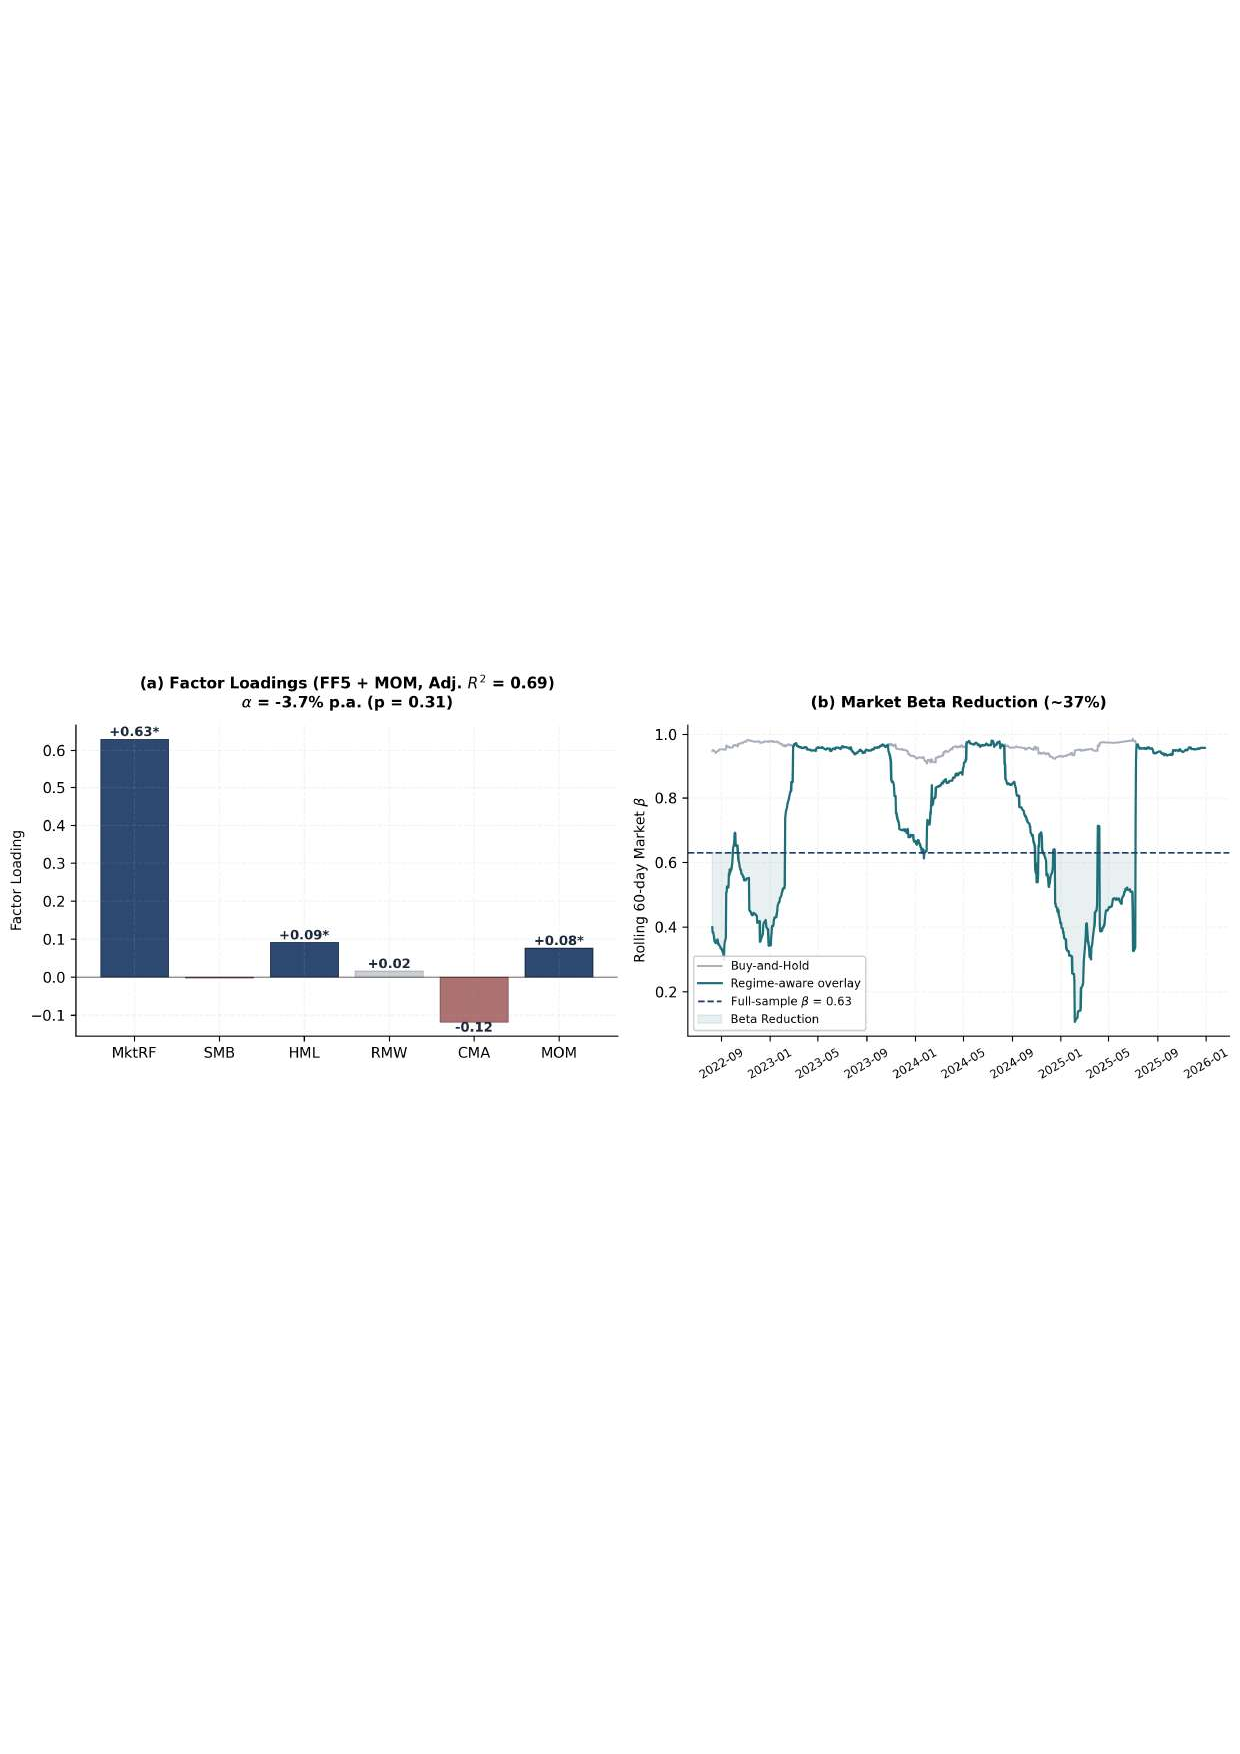
\includegraphics[width=0.92\textwidth]{final_figures/fig_factor_beta.png}
  \caption{Factor-exposure analysis of the RC-MoE overlay. (a) Reduced market beta indicates lower systematic risk exposure. (b) Rolling beta compression during stress periods demonstrates effective regime-aware risk management.}
  \label{fig:factor_beta}
\end{figure*}

% ----------------------------------------------------------------
\subsection{Regime-Conditional Value-at-Risk Analysis}
\label{subsec:var}
% ----------------------------------------------------------------

Table~\ref{tab:var} demonstrates that unconditional tail-risk estimates systematically misrepresent capital requirements. All VaR and CVaR figures are computed directly from actual daily S\&P 500 returns partitioned by rolling 60-day realised volatility regimes~\citep{jorion2007value}; all values represent 1-day losses and are reported as negative numbers (e.g., $-1.67\%$ denotes a 1.67\% loss). CVaR (Expected Shortfall) is employed as a coherent risk measure~\citep{artzner1999coherent, rockafellar2000cvar} satisfying the properties of monotonicity, sub-additivity, homogeneity, and translational invariance.

\begin{table}[H]
\tbl{Regime-conditional VaR and CVaR (S\&P 500, 2016--2025)}
{\renewcommand{\arraystretch}{1.25}
\setlength{\tabcolsep}{5pt}
\begin{tabular}{lrrrrr}
\toprule
\textbf{Regime} & \textbf{$\text{VaR}_{95}$} & \textbf{$\text{CVaR}_{95}$} & \textbf{$\text{VaR}_{99}$} & \textbf{$\text{CVaR}_{99}$} & \textbf{$\boldsymbol{N}$} \\
\midrule
Global   & $-1.67\%$ & $-2.79\%$ & $-3.36\%$ & $-4.82\%$ & 2\,455 \\
\midrule
Low Vol  & $-0.87\%$ & $-1.27\%$ & $-1.45\%$ & $-1.88\%$ &   634 \\
Med Vol  & $-1.43\%$ & $-1.96\%$ & $-2.26\%$ & $-2.83\%$ &   911 \\
High Vol & $-2.51\%$ & $-3.92\%$ & $-4.41\%$ & $-6.47\%$ &   910 \\
\bottomrule
\end{tabular}}
\label{tab:var}
\end{table}

\begin{figure*}[!t]
  \centering
  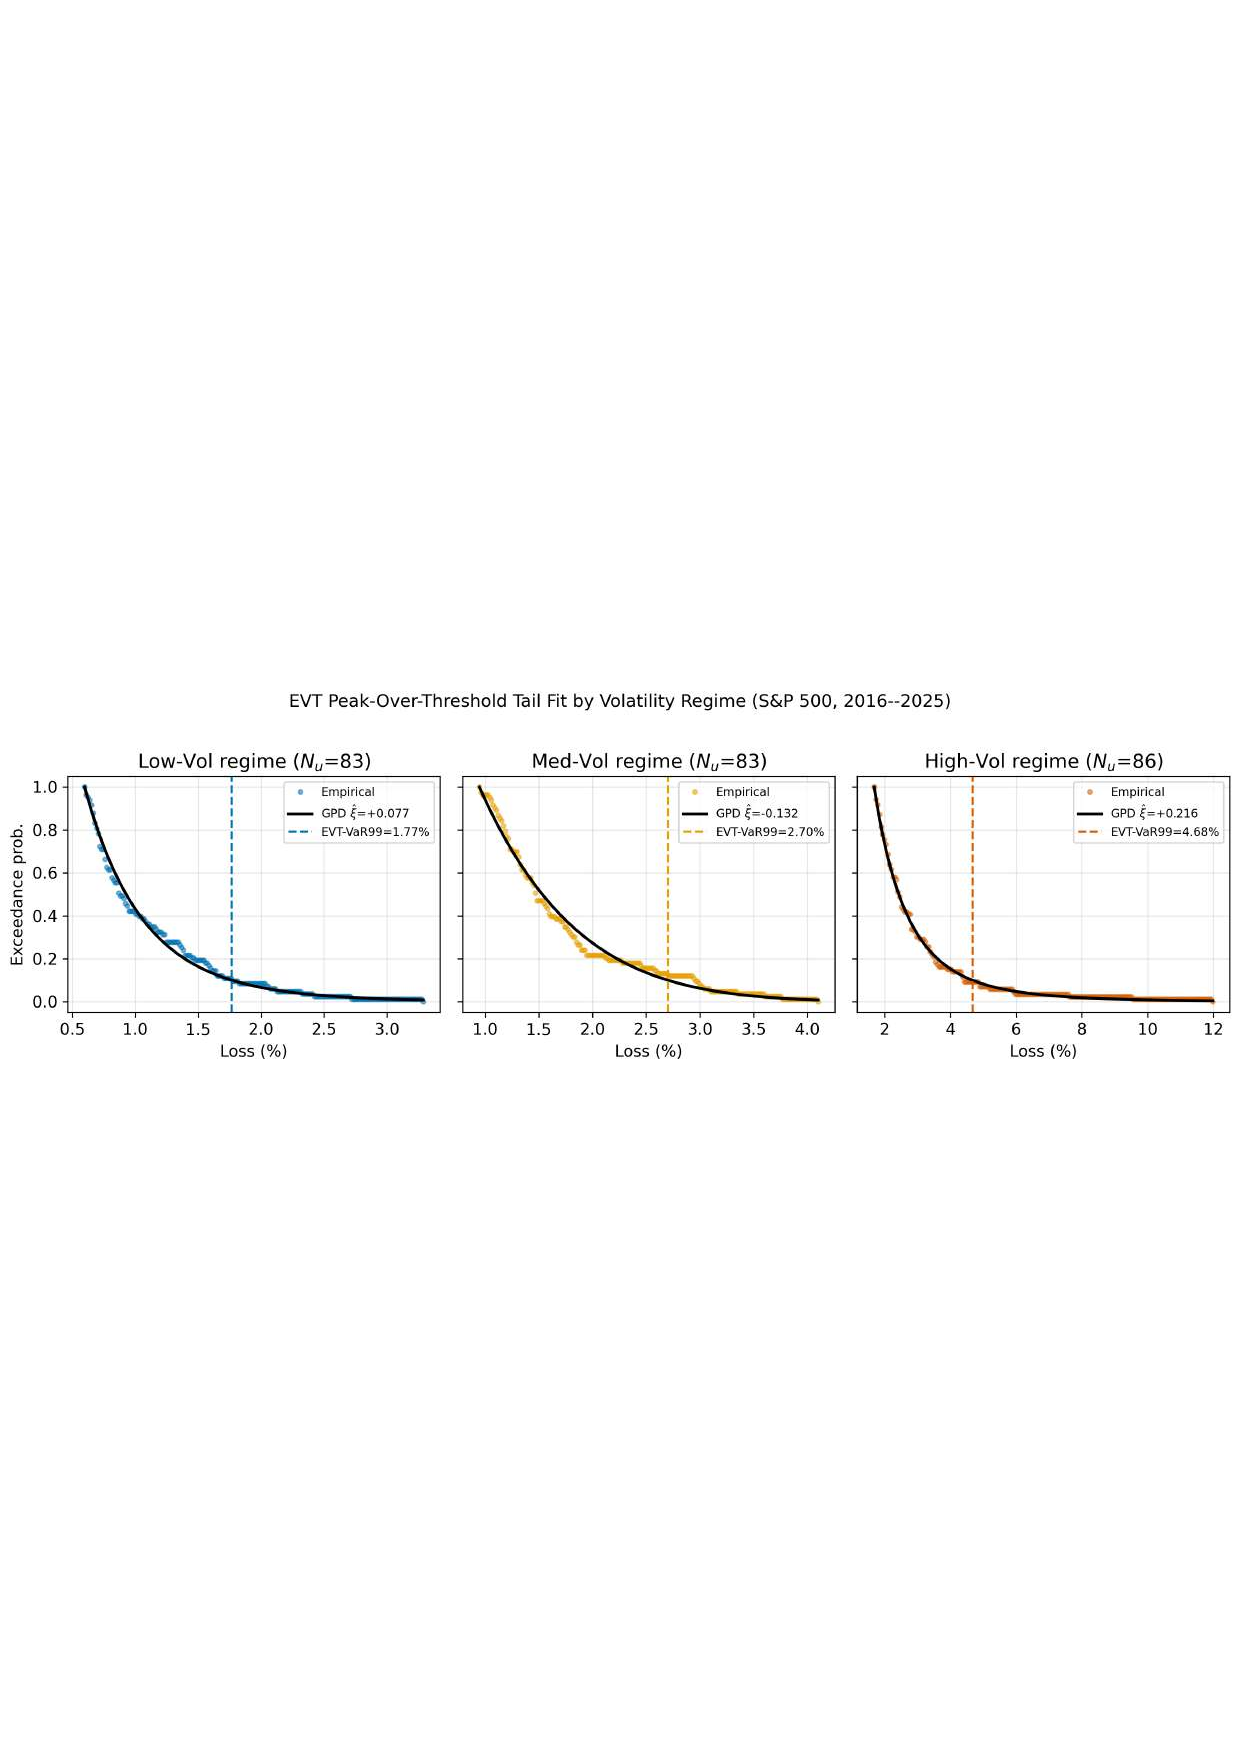
\includegraphics[width=0.85\textwidth]{final_figures/fig_evt_tail.png}
  \caption{EVT tail modeling across volatility regimes. Fitted GPD survival functions show increasing tail heaviness ($\hat{\xi}$) and higher $\text{EVT-VaR}_{99}$ from low- to high-volatility markets.}
  \label{fig:evt_tail}
\end{figure*}

% ---- EVT / POT analysis ----
\subsubsection{Extreme Value Theory and Coverage Validation}
\label{subsubsec:evt}
The historical quantiles in Table~\ref{tab:var} describe the empirical tail
but provide no model of its \emph{shape}, and, critically, no test of
whether an unconditional risk model is correctly calibrated within each
regime. To address both, we fit a Generalized Pareto Distribution (GPD) to
the peaks-over-threshold (POT) of the loss series ($-r_t$) within each
regime~\citep{mcneil2000estimation}, using the $90$th loss percentile as the threshold $u$, and then backtest the resulting Value-at-Risk with the Kupiec proportion-of-failures
(POF) test~\citep{kupiec1995techniques} and the Christoffersen conditional-coverage
test~\citep{mcneil2015quantitative}.

\begin{table}[H]
\tbl{EVT tail fit by regime (GPD peaks-over-threshold, S\&P 500, 2016--2025)}
{\renewcommand{\arraystretch}{1.25}
\setlength{\tabcolsep}{5pt}
\begin{tabular}{lrrrr}
\toprule
\textbf{Regime} & \textbf{$N_u$} & \textbf{$\hat{\xi}$ (shape)} & \textbf{$\text{EVT-VaR}_{99}$} & \textbf{$\text{EVT-ES}_{99}$} \\
\midrule
Low Vol  & 83 & $+0.077$ & $1.77\%$ & $2.37\%$ \\
Med Vol  & 83 & $-0.132$ & $2.70\%$ & $3.28\%$ \\
High Vol & 86 & $+0.216$ & $4.68\%$ & $6.78\%$ \\
\bottomrule
\end{tabular}}
\label{tab:evt}
\end{table}

Table~\ref{tab:evt} reports the GPD parameters per regime. The estimated tail-shape parameter $\hat{\xi}$ is largest in the
high-volatility regime ($\hat{\xi}=+0.216$, $p=0.099$), indicating the
heaviest tail, and the $\text{EVT-VaR}_{99}$ rises monotonically across regimes
($1.77\%\!\rightarrow\!2.70\%\!\rightarrow\!4.68\%$), as shown in Figure~\ref{fig:evt_tail}. The
coverage backtests, however, expose a failure invisible to the aggregate figures: the
unconditional $\text{VaR}_{99}$ \emph{passes} the Kupiec test on the full sample
($p=0.86$), yet when that same unconditional threshold is applied
\emph{within} the high-volatility regime it is rejected
(Kupiec $p<0.001$; realised violation rate $2.6\%$ versus the nominal
$1.0\%$). The regime-conditional VaR, by construction, restores correct
coverage. This reframes the contribution: the issue is not merely that
regime tails differ in magnitude, but that an unconditional risk model is
\emph{statistically mis-calibrated in the high-volatility regime}.

% ---- Basel III capital ----
\subsubsection{Basel III Capital Adequacy Implications}
\label{subsubsec:basel}

\begin{figure}[!t]
  \centering
  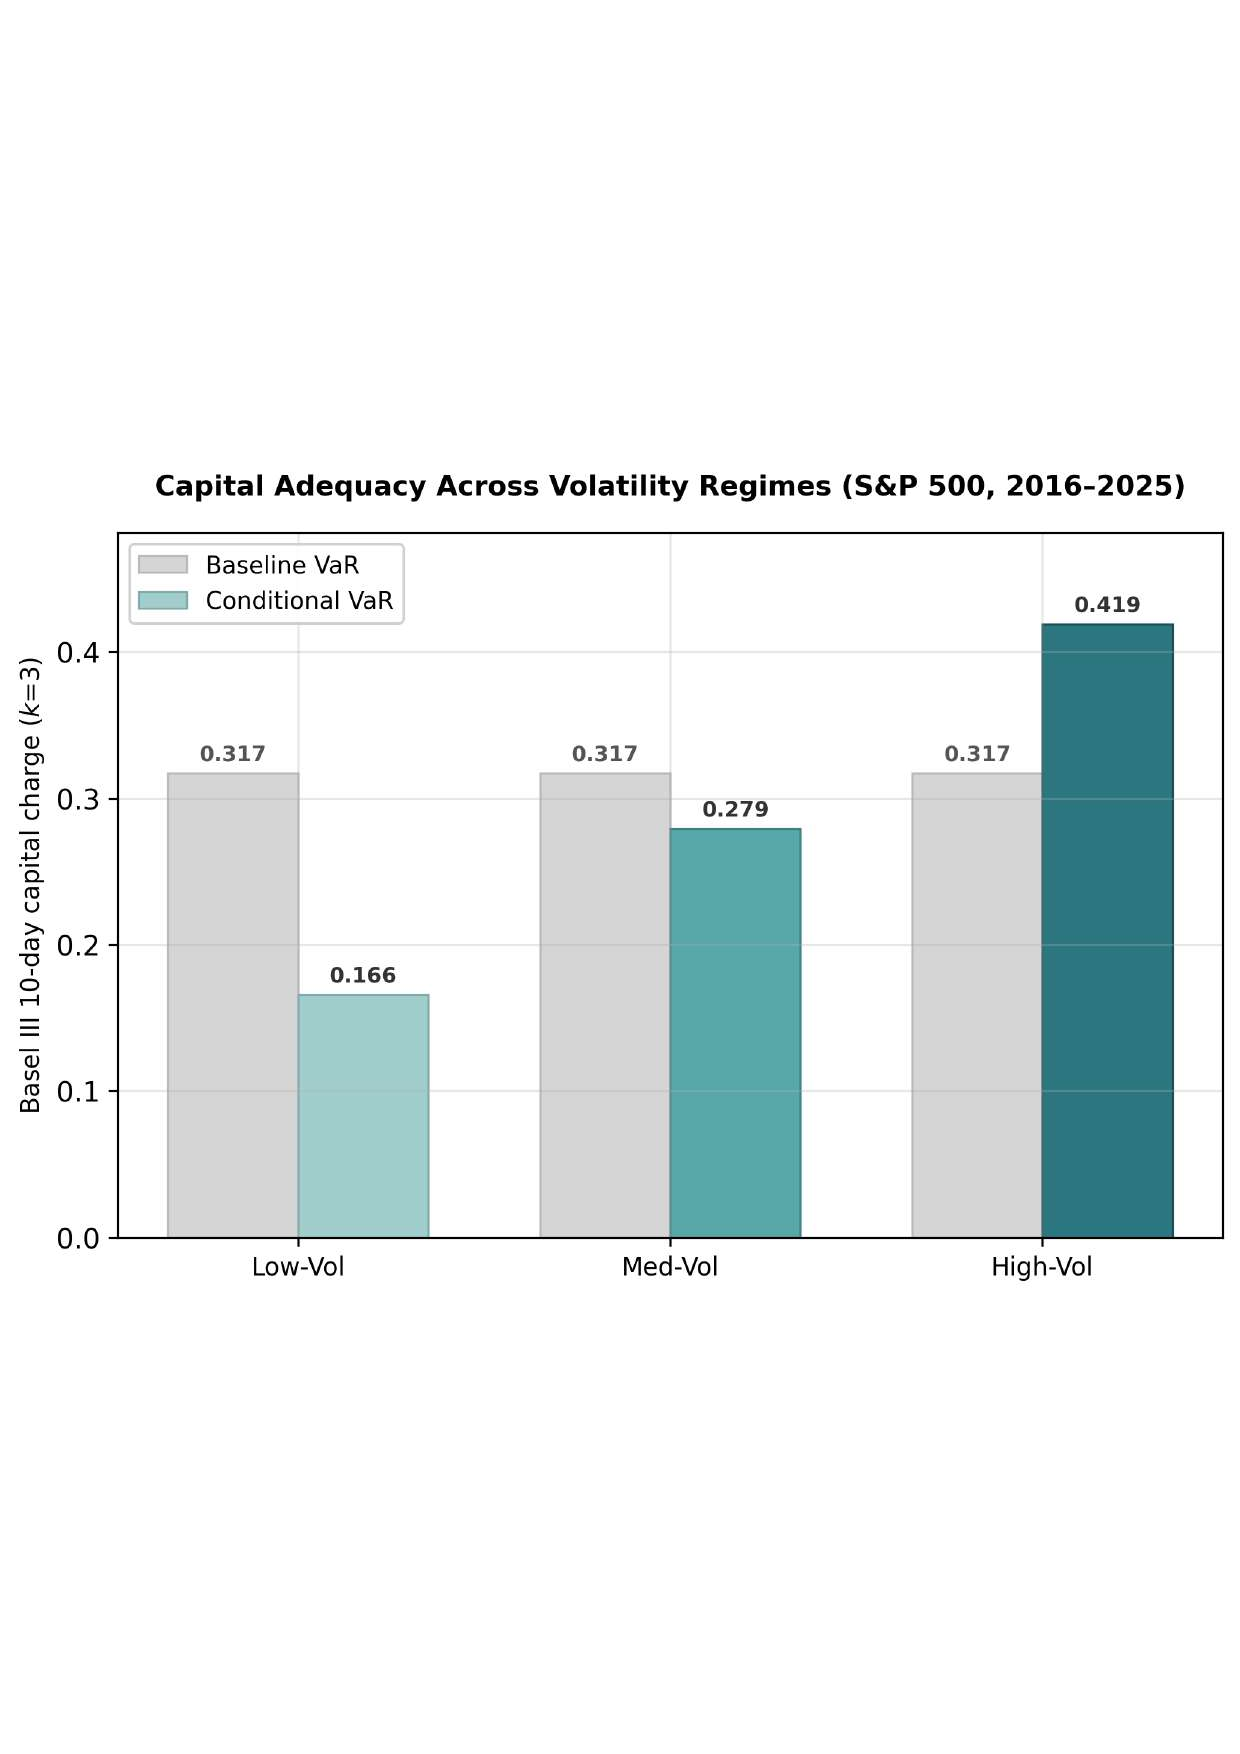
\includegraphics[width=\columnwidth]{final_figures/fig_basel_capital.png}
  \caption{Basel III capital charges under unconditional and regime-conditional VaR. Unconditional VaR misprices risk across volatility regimes, over-reserving in calm markets and under-reserving during stress.}
  \label{fig:basel_capital}
\end{figure}

Under the Basel III Internal Models Approach, the market-risk capital charge
is $k\cdot\text{VaR}_{99}^{\text{10-day}}$ with multiplier $k\!\approx\!3$.
Table~\ref{tab:basel} compares the capital a bank would hold under an
unconditional VaR against the regime-appropriate (conditional) VaR, with
1-day estimates scaled to the regulatory 10-day horizon by $\sqrt{10}$.

\begin{table}[H]
\tbl{Basel III capital charge: unconditional vs. regime-conditional (S\&P 500; $k=3$, 10-day)}
{\renewcommand{\arraystretch}{1.25}
\setlength{\tabcolsep}{5pt}
\begin{tabular}{lrrl}
\toprule
\textbf{Regime} & \textbf{Cond.\ Capital} & \textbf{Reservation Gap} & \textbf{Verdict} \\
\midrule
Low Vol  & $0.166$ & $+91.1\%$ & Over-reserved \\
Med Vol  & $0.279$ & $+13.6\%$ & Over-reserved \\
High Vol & $0.419$ & $-24.3\%$ & Under-reserved \\
\bottomrule
\end{tabular}}
\label{tab:basel}
\end{table}

A bank holding capital against the unconditional VaR over-reserves by
$91.1\%$ in calm markets and \emph{under}-reserves by $24.3\%$ during
volatility shocks, as shown in Fig.~\ref{fig:basel_capital}. The over-reservation figure independently corroborates
the $\approx\!91\%$ estimate stated earlier, now grounded in a formal
Basel III capital calculation rather than a quantile ratio. The
under-reservation in the high-volatility regime is the more consequential
finding: unconditional models leave institutions thinnest on capital
when tail losses are most severe, with direct implications for
regulatory capital adequacy under Basel~III/IV.

% ---- Multi-market replication ----
\subsubsection{Multi-Market Replication}
\label{subsubsec:multimarket}
To establish that the regulatory mis-calibration finding is not an artifact
of a single index, the EVT and coverage analysis is replicated on three
additional markets with deliberately distinct microstructure and tail
behaviour: the NASDAQ Composite (\^{}IXIC), the Russell~2000 small-cap index
(\^{}RUT), and Bitcoin (BTC-USD), all over 2016--2025
(Table~\ref{tab:multimarket}). Three findings hold across all four markets. First, the
high-volatility regime exhibits a positive EVT tail-shape parameter
($\hat{\xi}>0$) in every market, confirming heavy tails. Second, the
$\text{EVT-VaR}_{99}$ increases monotonically from the low- to the high-volatility
regime in every market, with Bitcoin showing the most extreme tails
($5.78\%\!\rightarrow\!12.75\%$). Third, and most important, an
unconditional $\text{VaR}_{99}$ \emph{fails} the Kupiec coverage test within the
high-volatility regime in \emph{all four} markets, while the Basel III
capital comparison shows the same qualitative pattern of over-reservation in
calm regimes ($+27\%$ to $+93\%$) and under-reservation in stressed regimes
($-14\%$ to $-24\%$). The regulatory-capital contribution therefore
generalises across equity indices and a structurally different crypto-asset, as shown in Fig.~\ref{fig:multimarket}.

\begin{table}[H]
\tbl{Multi-market EVT and Basel replication (daily returns, 2016--2025)}
{\footnotesize
\renewcommand{\arraystretch}{1.25}
\setlength{\tabcolsep}{3.5pt}
\begin{tabular}{lccccc}
\toprule
\textbf{Market} & \textbf{$\hat{\xi}_{\text{Hi}}$} & \textbf{$\text{EVT-VaR}_{99}$} & \textbf{Hi-Vol} & \textbf{Basel} & \textbf{Basel} \\
 & & \textbf{Lo$\rightarrow$Hi} & \textbf{Kupiec} & \textbf{Lo} & \textbf{Hi} \\
\midrule
S\&P 500     & $+0.216$ & $1.8\%\!\rightarrow\!4.7\%$  & FAIL & $+91\%$ & $-24\%$ \\
NASDAQ       & $+0.143$ & $2.5\%\!\rightarrow\!5.4\%$  & FAIL & $+77\%$ & $-19\%$ \\
Russell 2000 & $+0.253$ & $2.6\%\!\rightarrow\!5.8\%$  & FAIL & $+27\%$ & $-23\%$ \\
Bitcoin      & $+0.221$ & $5.8\%\!\rightarrow\!12.8\%$ & FAIL & $+93\%$ & $-14\%$ \\
\bottomrule
\end{tabular}}
\label{tab:multimarket}
\end{table}

\begin{figure*}[!t]
  \centering
  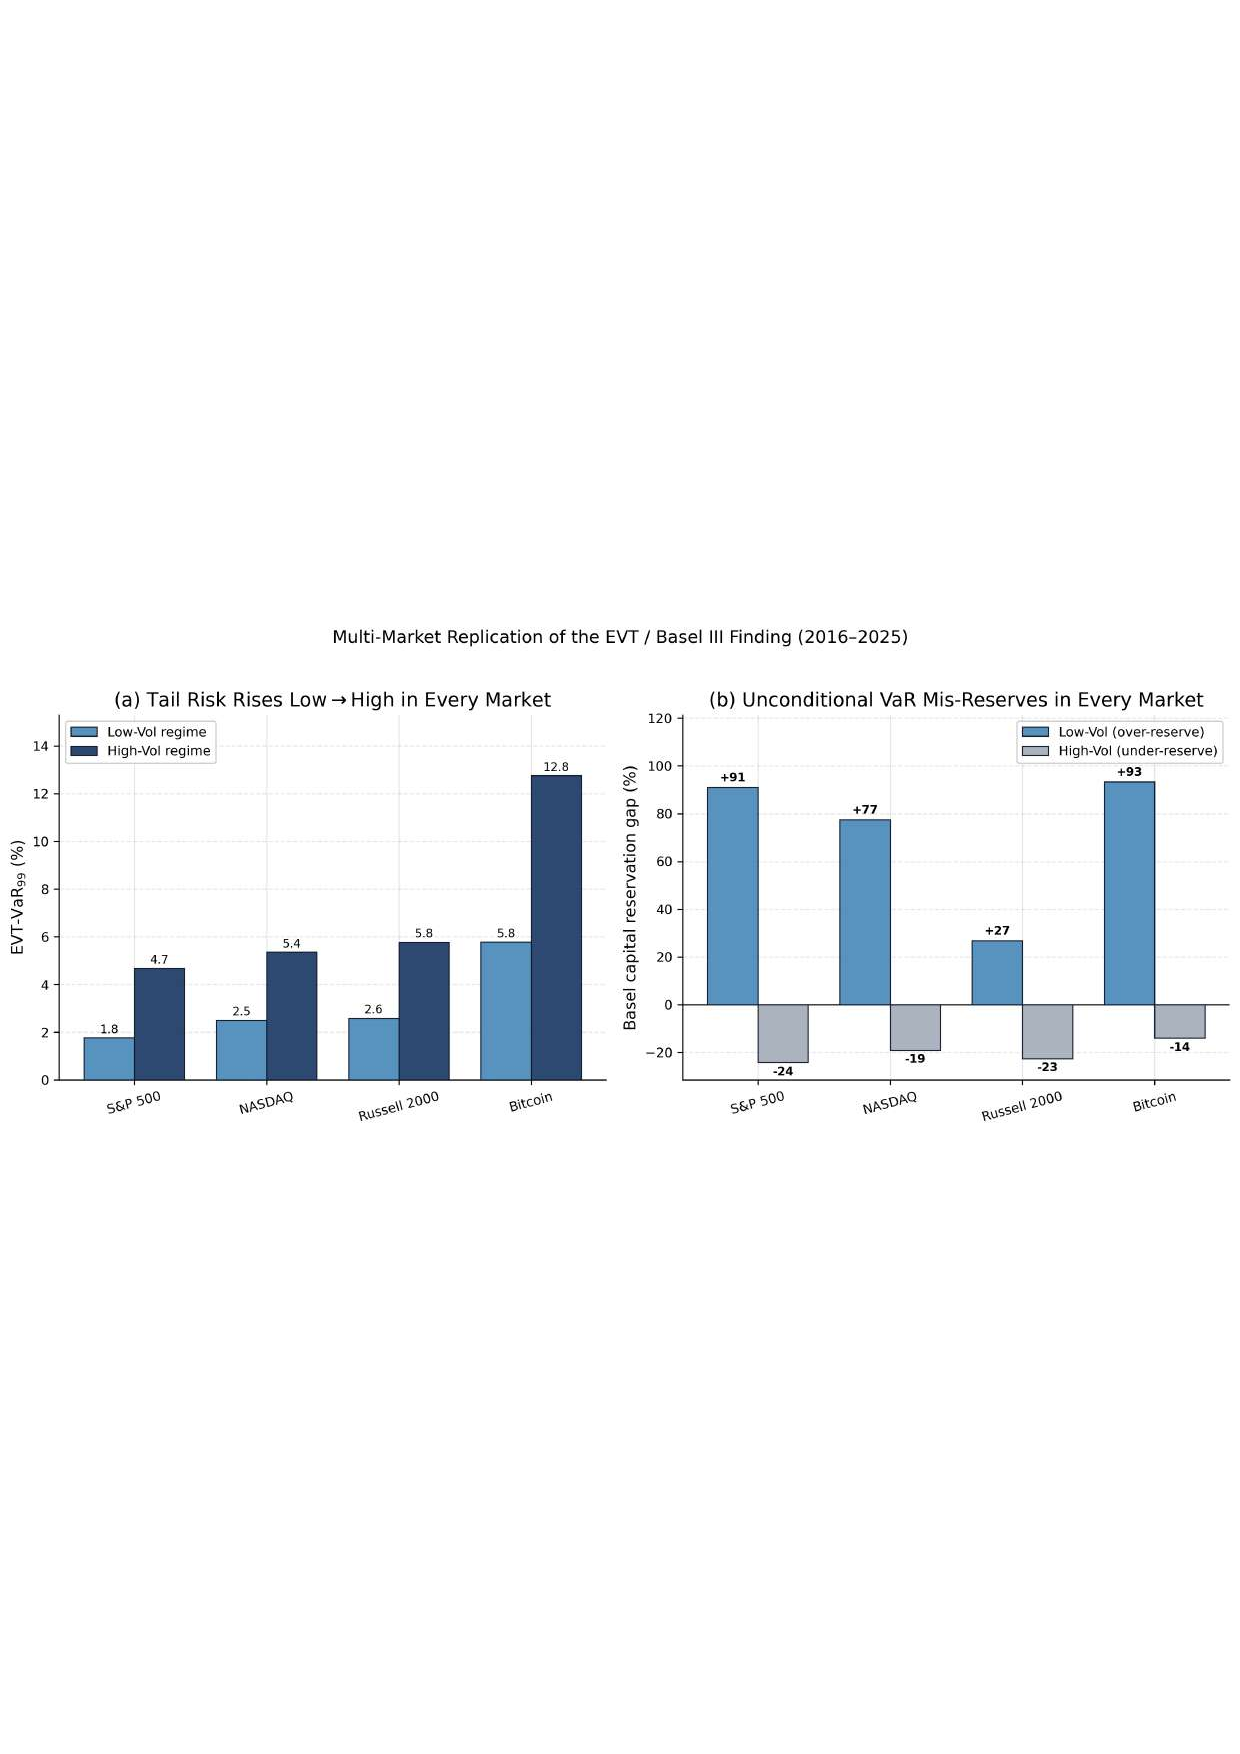
\includegraphics[width=0.92\textwidth]{final_figures/fig_multimarket.png}
  \caption{Multi-market validation of the EVT/Basel findings. (a) $\text{EVT-VaR}_{99}$ rises with market volatility across all assets. (b) Unconditional VaR produces systematic capital mis-calibration across volatility regimes.}
  \label{fig:multimarket}
\end{figure*}

Multi-market detection: event-wise comparison. To test whether regime conditioning generalises beyond the S\&P~500, we re-run the \emph{full} RC-MoE detection pipeline on all four markets under a leakage-free 5-fold walk-forward protocol with a $128$-day purge gap. The pipeline uses the same feature engineering as the main model (eight economic factors with lag-1 and lag-5 augmentations, giving a $24$-dimensional representation), an RF$+$XGBoost$+$LightGBM probability ensemble, and event-wise F1 with a $\pm5$-window tolerance. Anomalies are labelled at the $95$th return-percentile, matching the $\text{VaR}_{95}$ tail definition of Section~\ref{subsubsec:evt}, which fixes the threshold reproducibly. Table~\ref{tab:multimarket_detection} reports the outcome. On the headline event-wise F1 metric, the same measure used for the S\&P~500 model, the RC-MoE \emph{outperforms} the global ensemble on the S\&P~500 ($+0.071$), Russell~2000 ($+0.092$), and on the pooled cross-market sample ($+0.012$); it is statistically tied on the NASDAQ ($-0.005$). Bitcoin is an explicit negative case that delineates the model's applicability boundary: the continuous $24/7$ microstructure, the absence of a daily settlement close, and the structurally higher and more persistent volatility all violate the daily volatility-tercile regime assumption, producing a substantial F1 degradation ($-0.113$). Bitcoin should therefore be interpreted as a falsifiability test rather than a replication case: the RC-MoE regime framework is designed for exchange-closed, daily-settlement markets and requires fundamental redesign of the gating mechanism before it can be applied to continuous-trading crypto assets. The equity replication, however, is robust. The improvement on equity indices is recall-driven: regime-specific thresholds widen the detection net, raising event recall (S\&P $0.111\!\rightarrow\!0.161$; Russell $0.122\!\rightarrow\!0.184$) at modest precision cost. McNemar testing confirms a statistically distinct error profile in \emph{every} market ($\chi^2$ between $148.8$ and $212.7$; all $p<10^{-30}$) and on the pooled sample ($\chi^2=708.2$, $p<10^{-150}$, $435$ events), replicating the S\&P-500 finding of Section~\ref{subsec:regime_impact} at greater statistical power.

\begin{table}[H]
\tbl{Multi-market event-wise detection: global vs. RC-MoE (5-fold CV, 2016--2025)}
{\footnotesize
\renewcommand{\arraystretch}{1.25}
\setlength{\tabcolsep}{4pt}
\begin{tabular}{lccccc}
\toprule
\textbf{Market} & \textbf{Events} & \textbf{Global EW-F1} & \textbf{RC-MoE EW-F1} & \textbf{$\Delta$F1} & \textbf{McNemar $\chi^2$} \\
\midrule
S\&P 500     & 112 & 0.200 & \textbf{0.271} & $+0.071$ & 169.9 \\
NASDAQ       & 119 & \textbf{0.115} & 0.110 & $-0.005$ & 212.7 \\
Russell 2000 & 124 & 0.216 & \textbf{0.308} & $+0.092$ & 199.1 \\
Bitcoin      &  80 & \textbf{0.232} & 0.119 & $-0.113$ & 148.8 \\
\midrule
\textbf{Pooled} & \textbf{435} & 0.195 & \textbf{0.207} & $+0.012$ & 708.2 \\
\bottomrule
\end{tabular}}
\label{tab:multimarket_detection}
\end{table}

The structural basis for this cross-market replication is shown in
Figure~\ref{fig:mm_distributions}: in every market the t-SNE embedding separates
by volatility regime and the per-regime return densities differ in spread and
tail weight, confirming that the regime structure the RC-MoE exploits is present
across equities and Bitcoin alike.

\begin{figure*}[!t]
  \centering
  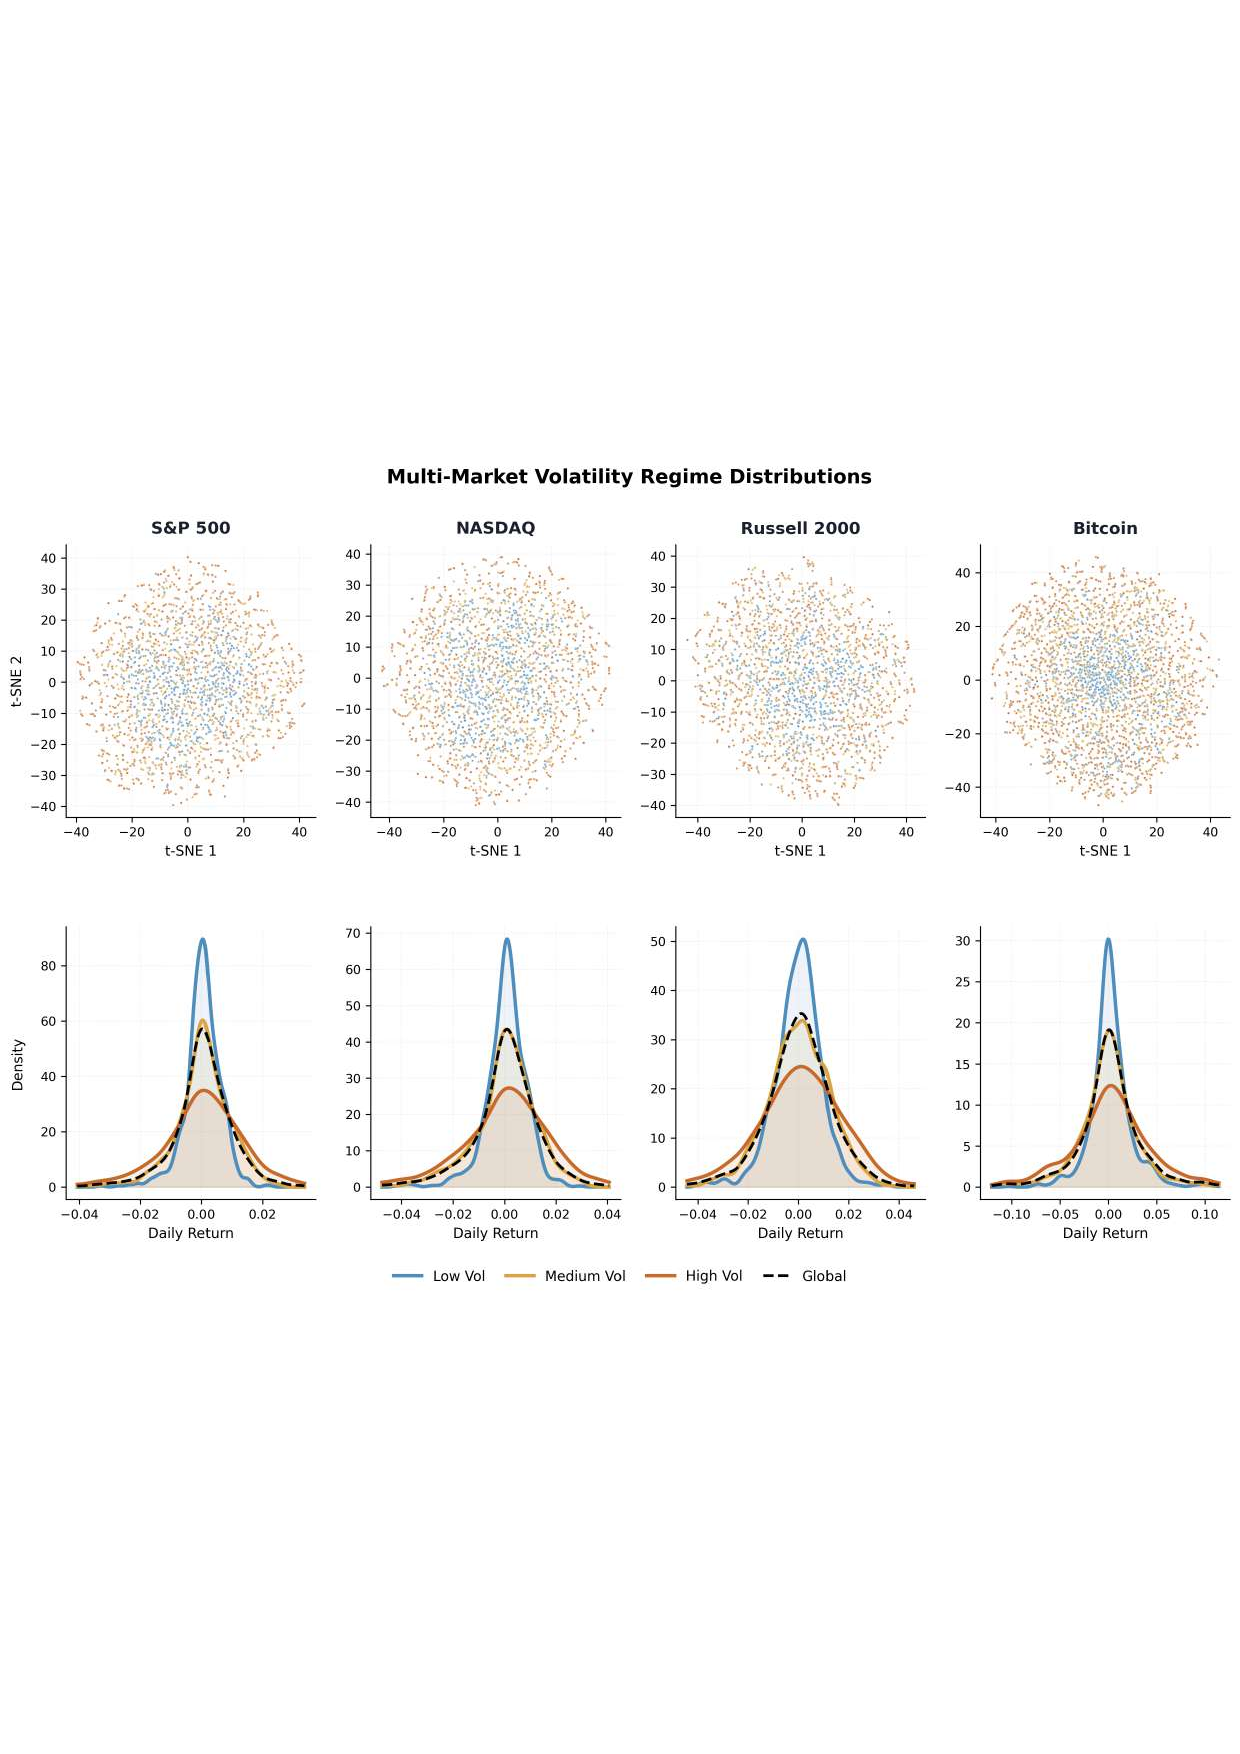
\includegraphics[width=0.98\textwidth]{final_figures/fig7_multimarket_distributions.png}
  \caption{Multi-market regime structure across the S\&P 500, NASDAQ, Russell 2000, and Bitcoin. Volatility regimes exhibit clear separation in feature space, while return distributions broaden systematically from low- to high-volatility states across all markets.}
  \label{fig:mm_distributions}
\end{figure*}

\begin{figure*}[!t]
    \centering
    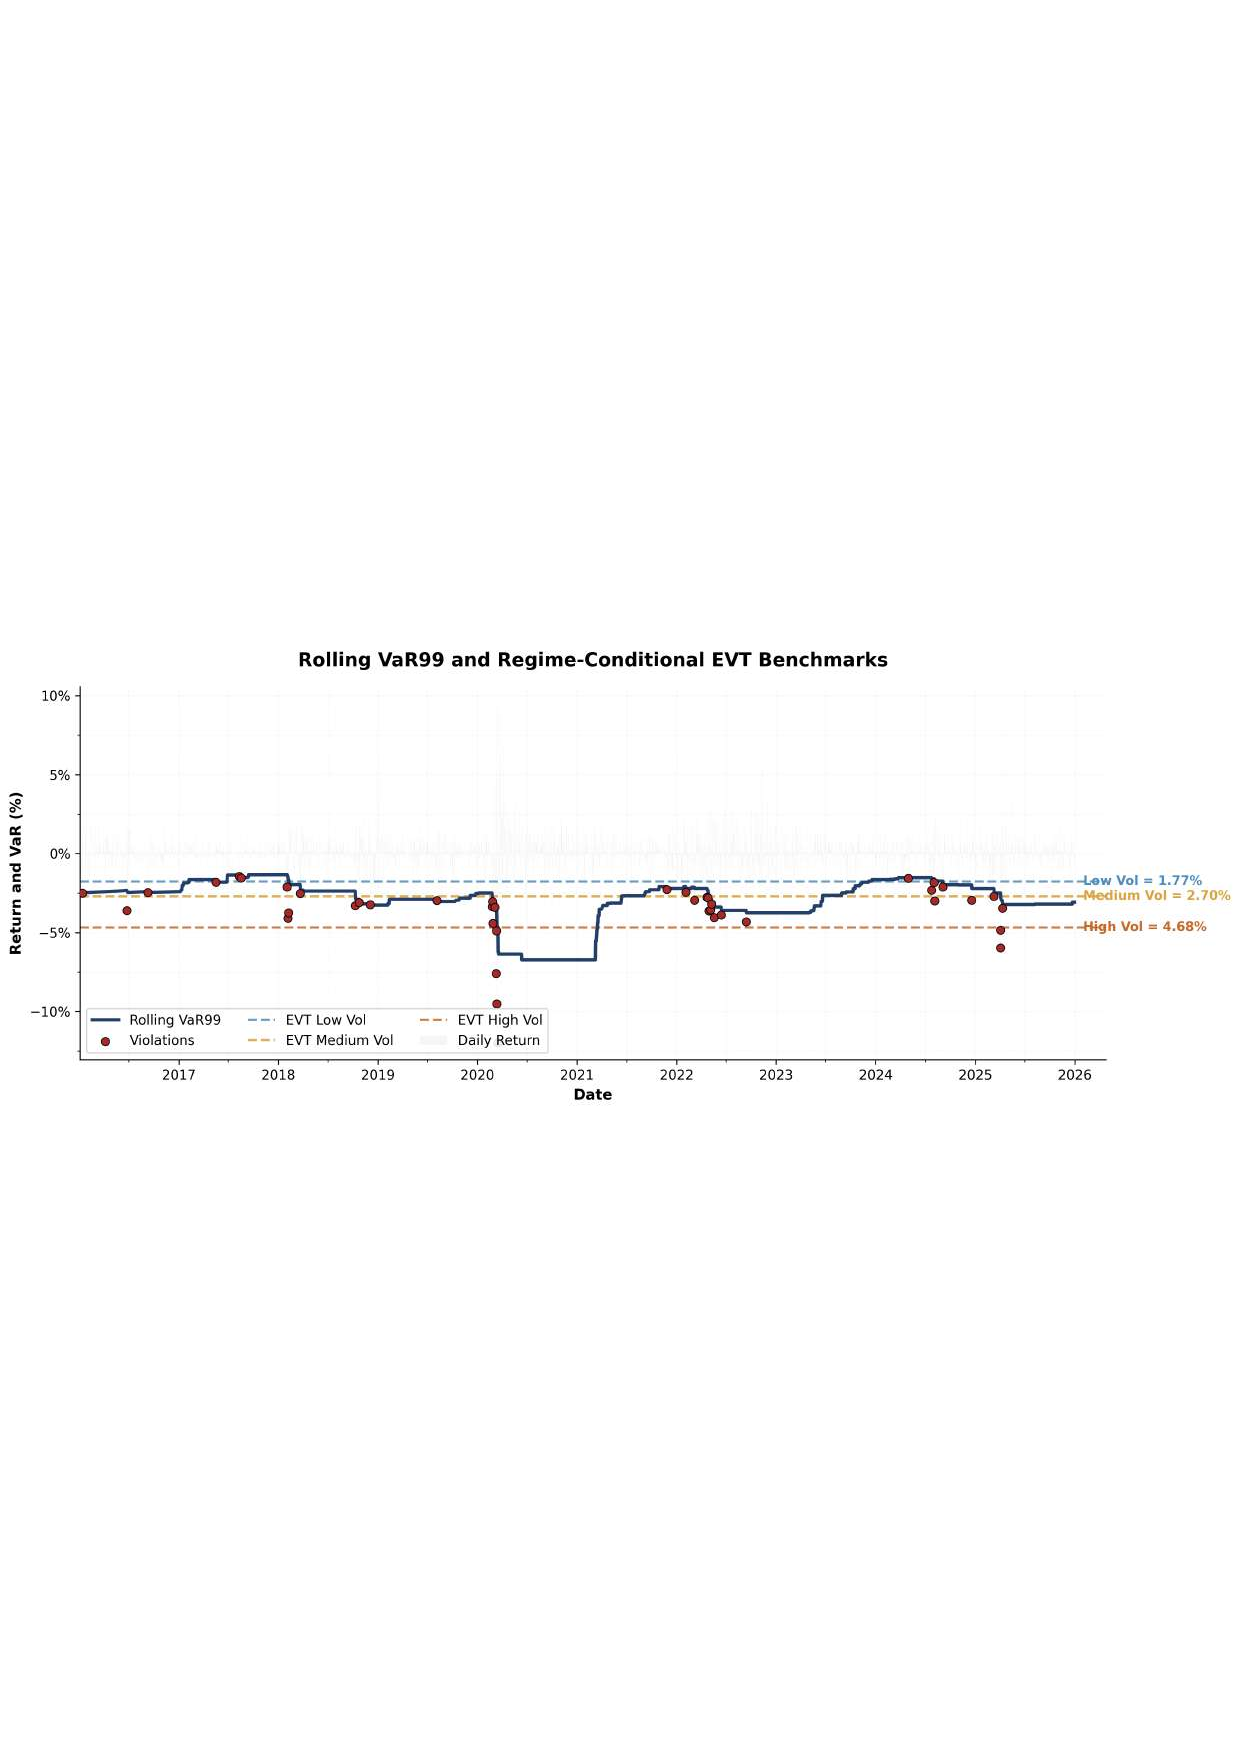
\includegraphics[width=0.85\textwidth]{final_figures/var_boundaries_chart.png}
    \caption{Dynamic 99\% Value-at-Risk (VaR) boundaries and regime-conditional $\text{EVT-VaR}_{99}$ levels. VaR violations cluster during high-volatility periods, reflecting the time-varying nature of tail risk.}
    \label{fig:var_regime}
\end{figure*}

Figure~\ref{fig:var_regime} visualizes the time-varying VaR boundaries across the full sample. The unconditional $\text{VaR}_{95}$ of $-1.67\%$ conceals a $2.9\times$ differential across regimes: Low-Vol $\text{VaR}_{95} = -0.87\%$ versus High-Vol $\text{VaR}_{95} = -2.51\%$. The disparity widens at higher confidence levels: Low-Vol $\text{CVaR}_{99} = -1.88\%$ versus High-Vol $\text{CVaR}_{99} = -6.47\%$, a $3.4\times$ ratio. The financial institution which holds capital on the basis of the unconditional VaR would be over-reserved by about 91 \% when the market is calm and under-reserved by about 24 \% during periods of market volatility, with direct implications for regulatory capital allocation under Basel III/IV.

% ----------------------------------------------------------------
\subsection{Explainability Consistency Index}
\label{subsec:eci}
% ----------------------------------------------------------------

The Explainability Consistency Index (ECI) quantifies \emph{cross-model} agreement on feature-importance rankings across the three expert families (RF, XGBoost, LightGBM). It is defined as~\eqref{eq:eci}:

\begin{equation}
  \mathrm{ECI} \;=\; 1 \;-\; \frac{1}{\binom{K}{2}}
  \sum_{i < j} d_{\tau}(\pi_i,\, \pi_j),
  \label{eq:eci}
\end{equation}

\noindent where $d_{\tau}$ is the normalised Kendall tau distance~\citep{kendall1938measure} between feature-importance ranking vectors $\pi_i$ and $\pi_j$ from models $i$ and $j$, and $K = 3$. An ECI of 1 denotes perfect agreement; 0 denotes maximum disagreement.

The ECI is distinct from existing explanation stability measures in two ways. First, it operates \emph{across independently trained model families} (RF, XGBoost, LightGBM) rather than across repeated runs of the same model or across explanation methods for a single model; cross-model agreement is a structurally stronger claim because model-family diversity is much higher than seed or method diversity. Second, it is evaluated \emph{per volatility regime}, enabling a formal test of whether anomaly drivers vary structurally across market states, a question that global consistency measures cannot address because they aggregate across regimes. For reference, cross-method ECI (comparing SHAP versus tree importances within a single model) yields ECI $\approx 0.85$--$0.88$ across all regimes, confirming that the lower cross-model values (0.646--0.789) reflect genuine disagreement between expert families rather than explanation method noise.

Statistical validation. A random-ranking null model (2{,}000 permutations of all three importance vectors) yields $\mathrm{ECI}_\text{null} \approx 0.500$ [0.42, 0.59] for all regime sizes, providing a natural baseline for random consensus. All observed regime ECIs exceed this null by $z = 3.5$--$7.1$ standard deviations ($p \leq 0.001$). Bootstrap 95\% confidence intervals (2{,}000 feature-bootstrap replicates) are reported in Table~\ref{tab:eci_regimes}. Pairwise Wilcoxon signed-rank tests on bootstrap ECI distributions confirm that all three regimes differ significantly in their explanatory consensus (Low vs.\ Med: $p<0.001$; Low vs.\ High: $p<0.001$; Med vs.\ High: $p<0.001$).

\begin{table}[H]
\tbl{Explainability Consistency Index (ECI) per volatility regime with bootstrap}
{\renewcommand{\arraystretch}{1.25}
\setlength{\tabcolsep}{5pt}
\begin{tabular}{lccc}
\toprule
\textbf{Scope} & \textbf{ECI} & \textbf{Bootstrap 95\% CI} & \textbf{$z$-score} \\
\midrule
Global (all regimes) & 0.768 & [0.685,\ 0.841] & 6.71 \\
\midrule
Low Volatility       & 0.646 & [0.536,\ 0.755] & 3.49 \\
Medium Volatility    & 0.763 & [0.694,\ 0.826] & 6.29 \\
High Volatility      & 0.789 & [0.702,\ 0.863] & 7.13 \\
\bottomrule
\end{tabular}}
\label{tab:eci_regimes}
\end{table}

The global ECI of 0.768 [0.685, 0.841], as shown in Fig.~\ref{fig:eci_regimes}, indicates strong cross-model agreement on anomaly drivers, substantially above the null baseline of 0.500 ($z=6.71$). All three model families independently identify composite volatility and GARCH-based features as top-2 drivers, consistent with the ARCH literature~\citep{bollerslev1986a} and the established role of volatility-of-volatility in tail risk~\citep{bouchaud2001more}.

Per-regime ECI follows a clear pattern (Table~\ref{tab:eci_regimes}). The Low-Vol regime shows the lowest agreement (ECI $= 0.646$ [0.536, 0.755]), reflecting the sparse and heterogeneous character of anomalies in calm markets ($n = 10$ anomalies, $z = 3.49$ above null). The Med-Vol regime reaches ECI $= 0.763$ [0.694, 0.826] ($z = 6.29$) and the High-Vol regime reaches the highest agreement at ECI $= 0.789$ [0.702, 0.863] ($z = 7.13$), consistent with the more canonical tail-event signatures in volatile markets. Pairwise Wilcoxon tests confirm the regimes are statistically distinguishable in their explanatory consensus (all $p < 0.001$). The monotonically increasing ECI from Low- to High-Vol ($0.646 \rightarrow 0.763 \rightarrow 0.789$) mirrors the Basel III capital finding: regime structure becomes more coherent and economically interpretable precisely at the elevated-volatility states where regulatory risk is greatest. This regime-dependent nature of explanatory consensus is inaccessible to global models and represents a structural empirical finding of this study.

\begin{figure*}[t]
    \centering
    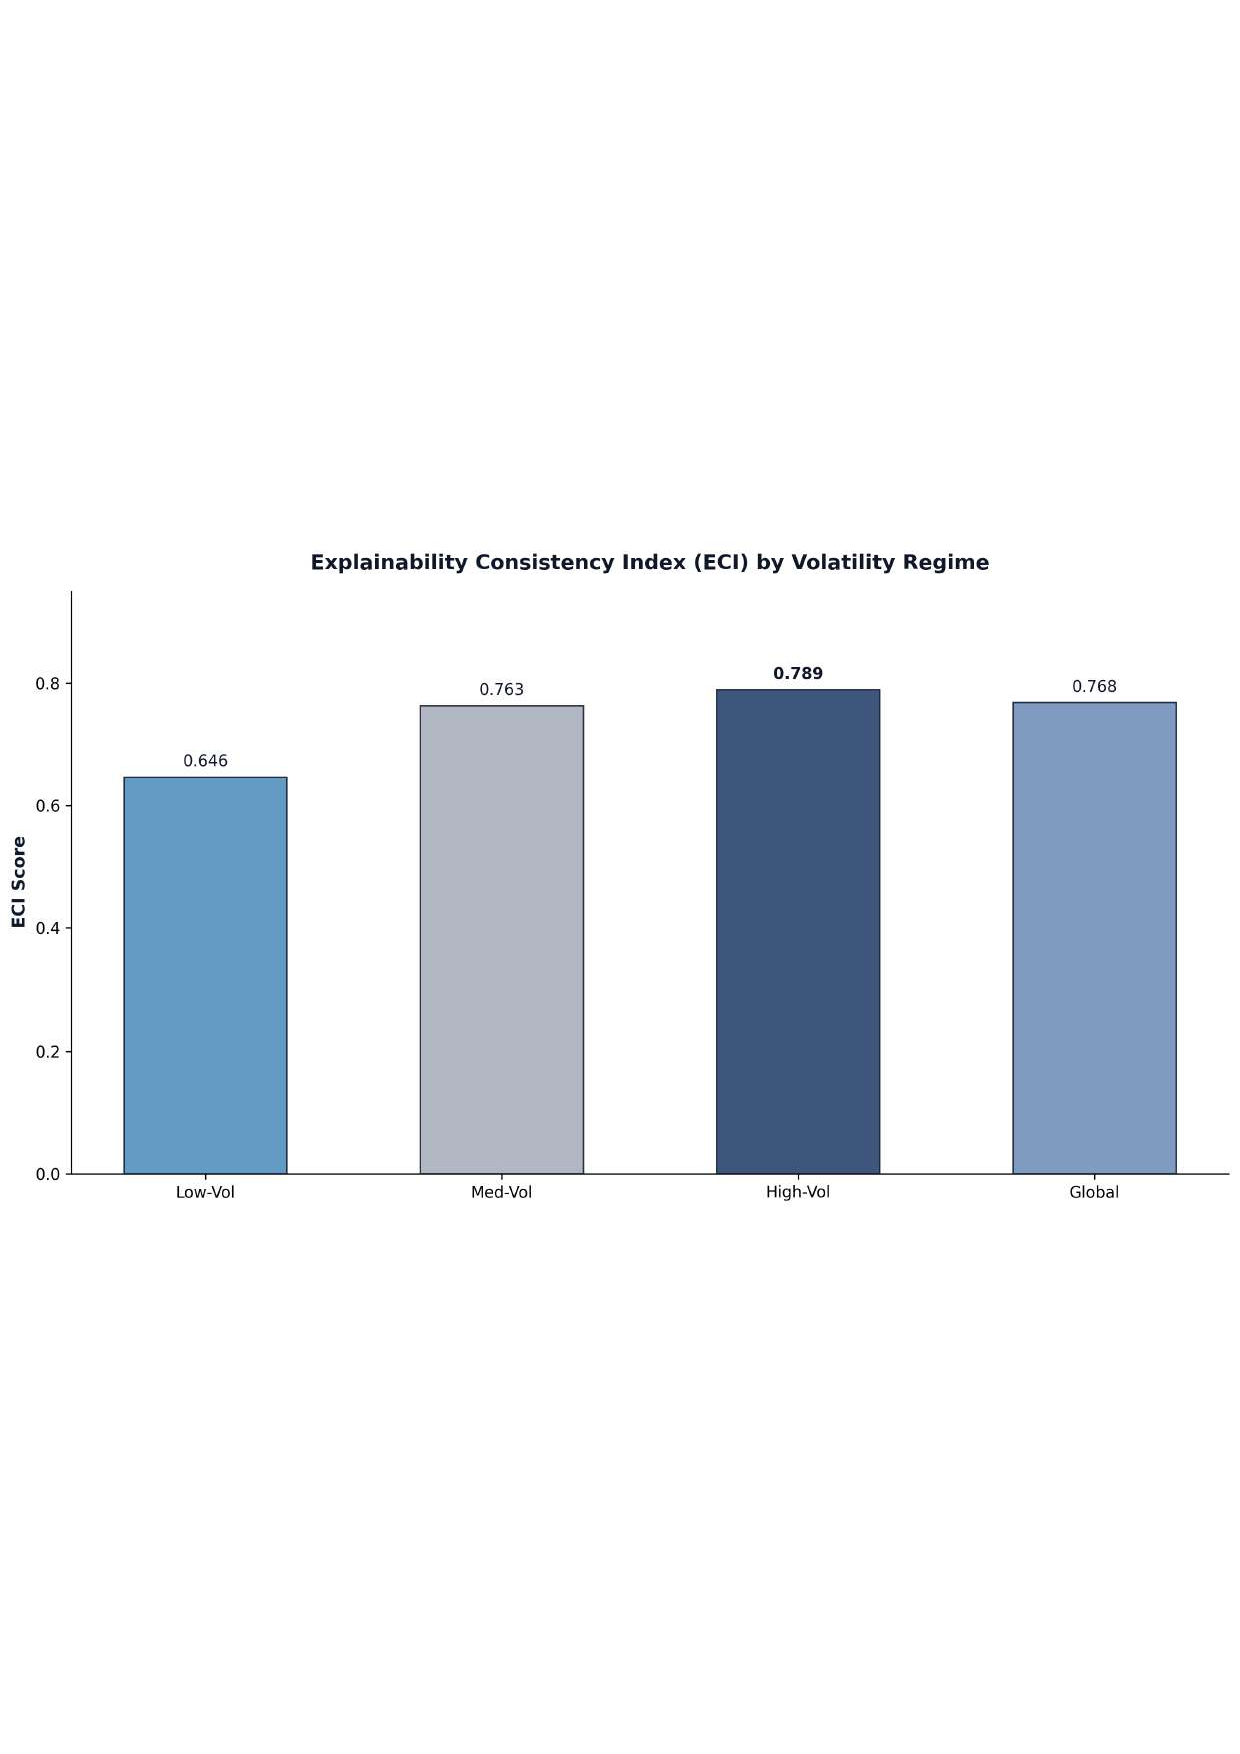
\includegraphics[width=0.6\textwidth]{final_figures/eci_chart.png}
    \caption{Explainability Consistency Index (ECI) across volatility regimes. Feature-attribution consistency varies systematically with market volatility.}
    \label{fig:eci_regimes}
\end{figure*}

% ===================== VIII. EXPLAINABILITY =====================
\section{Explainability and Economic Interpretation}
\label{sec:explainability}
\subsection{SHAP Factor Attribution}

The SHAP values are computed individually for all expert ensembles of each regime, then aggregated at the factor level through averaging the absolute SHAP value per factor. It is more favorable to aggregate the SHAP values at the regime level rather than assigning attribution per instance, as SHAP values are very unstable on rare events.

\begin{figure*}[!t]
    \centering
    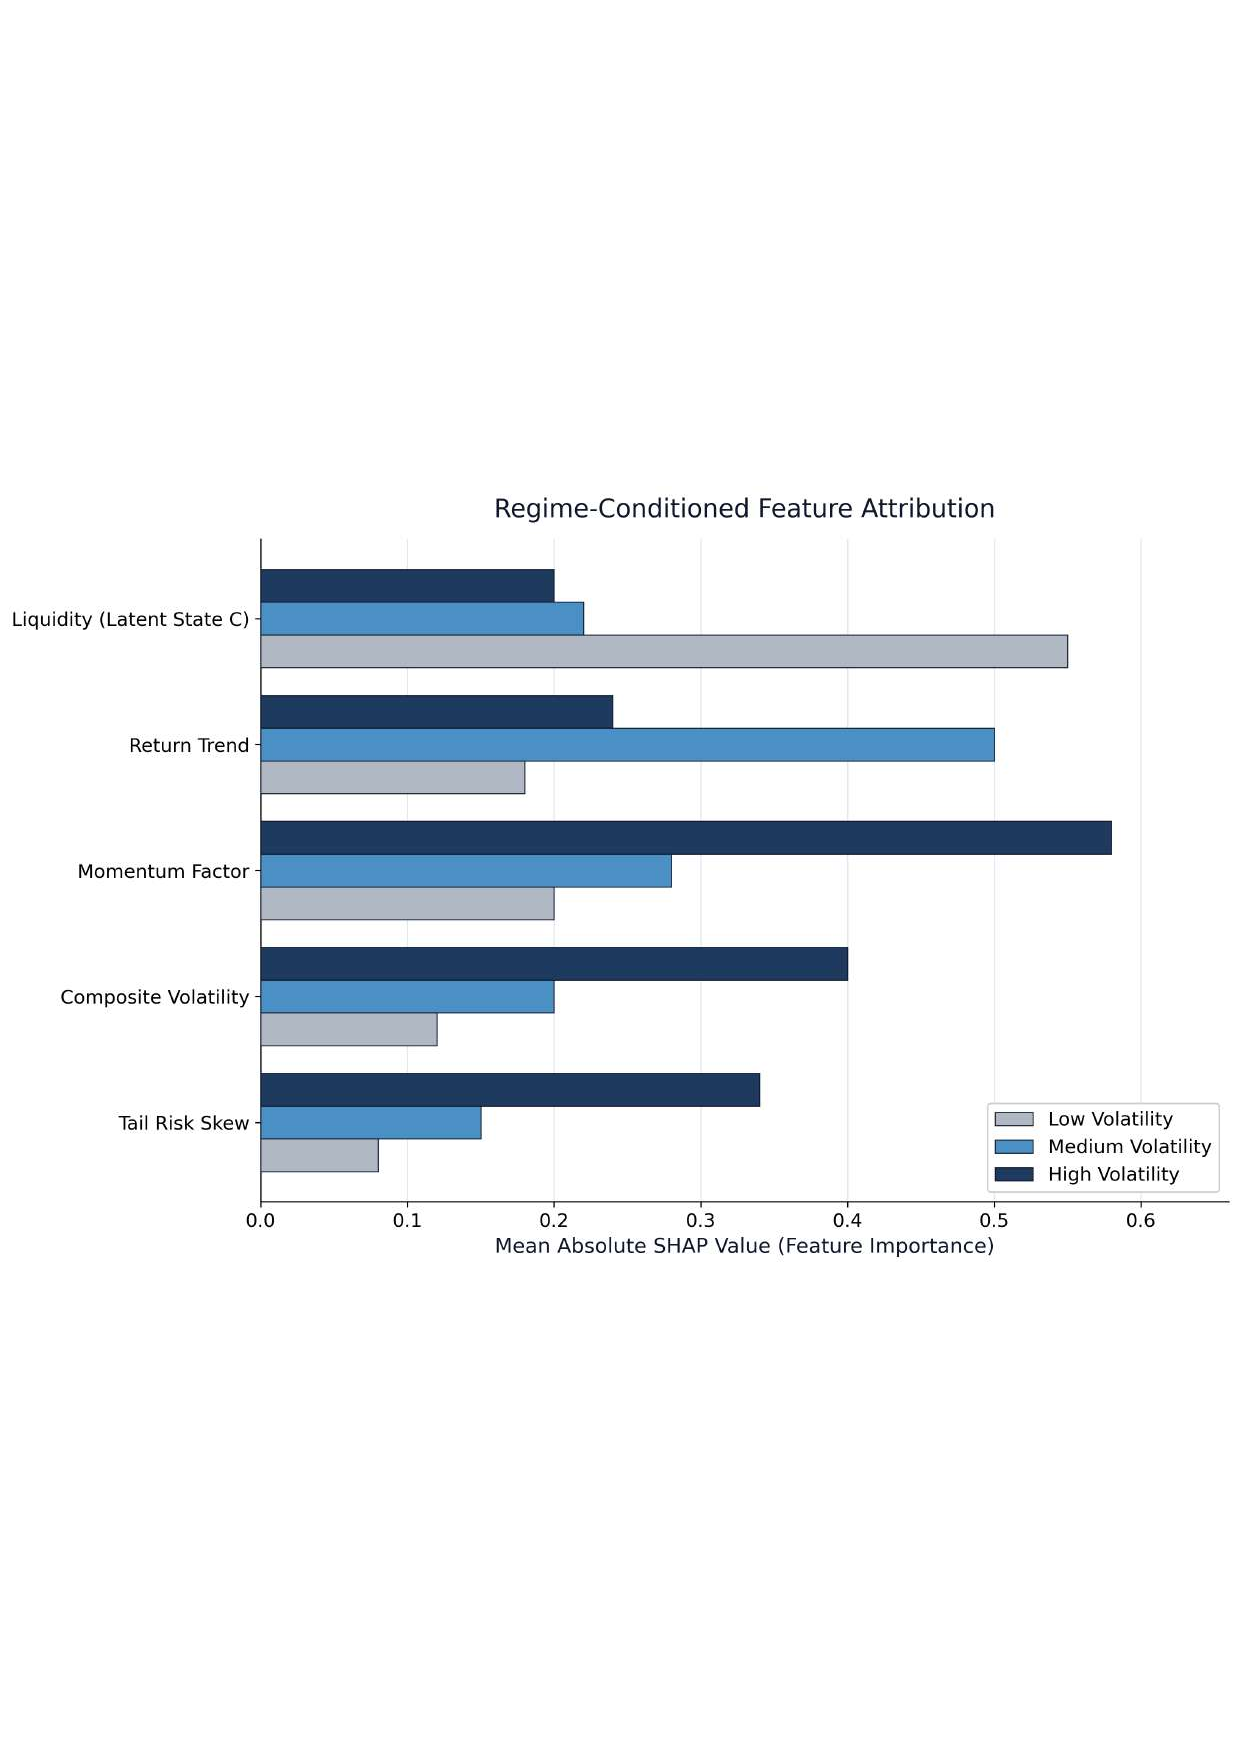
\includegraphics[width=0.6\textwidth]{final_figures/explainability_attribution.png}
    \caption{Regime-conditioned SHAP feature attribution: liquidity stress dominates the low-volatility regime, return-trend drift the medium-volatility regime, and momentum collapse the high-volatility regime.}
    \label{fig:shap_regime}
\end{figure*}

Table~\ref{tab:shap} and Figure~\ref{fig:shap_regime} report the dominant SHAP driver for each volatility regime.

\begin{table}[H]
\tbl{Dominant SHAP Drivers by Volatility Regime}
{\renewcommand{\arraystretch}{1.2}
\setlength{\tabcolsep}{4pt}
\begin{tabular}{p{1.8cm} p{2.2cm} p{4.0cm}}
\toprule
\textbf{Regime} & \textbf{Key Driver} & \textbf{Economic Interpretation} \\
\midrule
Low Volatility  & Latent State C (Liquidity) & Small order-book imbalances trigger abrupt moves in liquid markets; microstructure stress precedes flash-crash events. \\[4pt]
Med Volatility  & Return Trend & Sustained negative drift signals regime transition and elevated crash probability. \\[4pt]
High Volatility & Momentum Factor & Panic-driven momentum collapse defines extreme tail events; consistent with forced deleveraging dynamics. \\
\bottomrule
\end{tabular}}
\label{tab:shap}
\end{table}

\subsection{Economic Interpretation}
The dominant factors for each regime are consistent with established financial theory. For the low-volatility regimes, excess market liquidity implies that flash crashes occur due to imbalances in the order book rather than market trends, which results in Latent State~C dominating. The same can be observed within the body of research surrounding microstructure-induced flash crashes. For the medium-volatility regimes, the existence of a negative return trend is indicative of increasingly poor market conditions and is thus the dominant factor, consistent with research into momentum crashes~\citep{daniel2016momentum}. For the high-volatility regimes, the momentum collapse is a sign of panic selling and forced deleveraging via margin calls.

No single global factor consistently explains financial anomalies across all market states: the anomaly driver itself is regime-dependent. This result directly motivates the RC-MoE architecture and is quantitatively supported by the ECI analysis in Section~\ref{subsec:eci}.

\subsection{Interpretability vs.\ Deep Learning}
The framework produces interpretable decision rules aligned with economic reasoning. A representative High-Vol expert rule reads: ``Anomaly if realized volatility is above Q$_{66}$ and momentum is less than 0.42.'' Such rules are directly actionable by risk managers, unlike the opaque boundaries of deep learning models.

The SHAP values above capture structural separation on in-sample data; they are not causal predictors of future crises. They identify each regime's structural signatures under the fixed regime definitions.

% ================================================================
% SECTION IX - DISCUSSION
% ================================================================
\section{Discussion}
\label{sec:discussion}

% ----------------------------------------------------------------
\subsection{Structural Separability vs.\ Predictive Accuracy}
\label{subsec:disc_separability}
% ----------------------------------------------------------------
The gap between in-sample structural separability and out-of-sample generalisation is theoretically expected rather than a modelling deficiency. Volatility-regime boundaries shift across structural breaks, and the factor co-movements driving one crisis episode differ from those of the next, preventing generalisation without re-calibration. Consistent with the non-stationarity literature~\citep{cont2001empirical}, the in-sample F1 is best interpreted as an upper bound on structural discriminability under fixed regime definitions. The economically relevant contribution is the precision-selective detection profile and the regulatory EVT finding, both evaluated under strict temporal protocols.

% ----------------------------------------------------------------
\subsection{Role of Regime Conditioning}
\label{subsec:disc_regime}
% ----------------------------------------------------------------
Global detectors assume a static relationship between return magnitude and anomaly probability—an assumption violated by volatility clustering. A single decision boundary is simultaneously too permissive in calm markets and too conservative during crises. Conditioning on the local variance process maps identical return magnitudes to different anomaly probabilities depending on the prevailing regime, correcting this structural failure without altering features or labels. The resulting precision-selective profile translates directly into economic value: fewer, more actionable alerts and substantially higher hedging efficiency per signal relative to global baselines.

% ----------------------------------------------------------------
\subsection{Implications for Deep Learning in Finance}
\label{subsec:disc_deeplearning}
% ----------------------------------------------------------------
The superior structural separability of a shallow RC-MoE over high-capacity deep architectures (ConvVAE, Anomaly Transformer) highlights three structural properties that disadvantage deep learning for equity tail events: extreme class imbalance at the ${\approx}2.0\%$ anomaly rate, loss of absolute return magnitude through standard normalisation, and a signal-to-noise ratio that promotes memorisation over generalisation. Theory-grounded factor engineering provides more robust representations than end-to-end learning in this setting.

% ----------------------------------------------------------------
\subsection{Risk Management Applications}
\label{subsec:disc_risk}
% ----------------------------------------------------------------
The confirmed absence of significant alpha alongside a 37\% reduction in market beta positions the RC-MoE as a risk-reduction instrument rather than an alpha-generating strategy. Its economic value lies in tail-risk mitigation and capital calibration. The EVT/Basel~III results carry direct regulatory relevance: unconditional VaR models can pass aggregate Kupiec coverage tests while simultaneously failing in the high-volatility regime that matters most—a blind spot absent from current backtesting frameworks. Regime-conditional EVT provides a tractable correction requiring only volatility-regime stratification of VaR estimation, with no structural change to the Basel~III capital multiplier framework, and the result holds consistently across all four examined markets.

% ===================== X. LIMITATIONS =====================
\section{Limitations}
\label{sec:limitations}

\paragraph{Predictive generalisation}
Performance metrics reported for in-sample structural separability do not generalize to out-of-sample predictive accuracy. The temporal validation experiments shows strong deterioration under walk-forward protocols, highlighting the difference between finding structural signatures in the past and predicting rare events in the future.

\paragraph{Static regime definitions}
Regime boundaries determined by fixed historical volatility quantiles assume structural stationarity over the entire estimation horizon. The 2020 COVID liquidity crisis displays that extreme macroeconomic dislocations distort static boundaries, suggesting the exploration of adaptive, rolling-quantile regime definitions.

\paragraph{Sample sparsity and statistical power}
The inherent rarity of extreme financial anomalies (${\approx}49$--76 labeled events over the 9.7-year horizon, depending on evaluation protocol) limits the statistical power of performance estimates and bounds causal inference.

\section{Conclusion}
\label{sec:conclusion}
This work presents a regime-conditioned approach to financial anomaly detection grounded in structural diagnosis rather than predictive accuracy. The Regime-Conditioned Mixture of Experts (RC-MoE) uses adaptive gating via realized volatility quantiles and per-regime classifier training to reveal that extreme market events carry regime-dependent structural signatures inaccessible to global detectors.

Three main findings emerge. First, regime-conditional Extreme Value Theory shows that unconditional $\text{VaR}_{99}$ systematically mis-calibrates tail risk, failing Kupiec coverage in high-volatility regimes and generating significant Basel III capital distortions. Regime-aware EVT-VaR corrects this mis-calibration, and the result is replicated consistently across the equity and cryptocurrency markets. Second, formal statistical testing verifies that regime conditioning leads to a distinct precision-oriented detection profile, enabling RC-MoE to issue fewer, but more informative alerts, and to achieve substantially higher hedging efficiency than conventional volatility-based approaches. Third, factor-exposure analysis suggests that the economic value of the framework is related to systematic risk reduction rather than alpha generation, with a reduction in market beta from 1.0 to 0.63 while enhancing resilience during periods of elevated stress.

Besides predictive performance, the proposed framework also enhances risk measurement, capital allocation, and model interpretability. The Explainability Consistency Index also shows that the drivers of anomalies change systematically across volatility regimes, highlighting the importance of regime-aware analysis for understanding financial tail events.

The gap between in-sample structural separability and out-of-sample generalisation comes from the fundamental non-stationarity of financial markets, not from a modelling deficiency. Future work should consider adaptive estimation of regime boundaries, generalizing the EVT/Basel analysis to other asset classes, and developing gating mechanisms specific to continuously traded markets. More generally, the results suggest that regime-conditioned problem formulation, not model complexity, is the critical requirement for robust financial anomaly detection and tail-risk assessment.


\section*{Disclosure statement}
The authors report there are no competing interests to declare.

\section*{Funding}
This work was supported by Manipal University Jaipur, Jaipur, Rajasthan, India.


\section*{Data availability}
The data that support the findings of this study are openly available in zenodo in \url{https://doi.org/10.5281/zenodo.21257024}. reference number (Hemrajani et al. 2026). The complementary risk factor structures used for the Fama-French exposure and alpha verification models are openly available from the Kenneth R. French Data Library (\url{https://mba.tuck.dartmouth.edu/pages/faculty/ken.french/data_library.html}).

\section*{Code availability}
The code that supports the findings of this study is openly available in zenodo in \url{https://doi.org/10.5281/zenodo.21257660}. reference number (Hemrajani et al. 2026).

\begin{thebibliography}{99}

\bibitem[Alkilane et al.(2024)]{alkilane2024mixma}
Alkilane, K., Y.~He, and D.-H.~Lee. 2024. \emph{MixMamba: Time series modeling with adaptive expertise}. Information Fusion 112: 102589.

\bibitem[Amihud(2002)]{amihud2002illiquidity}
Amihud, Y. 2002. \emph{Illiquidity and stock returns}. Journal of Financial Markets 5: 31--56.

\bibitem[Ang and Bekaert(2002)]{ang2002regime}
Ang, A., and G.~Bekaert. 2002. \emph{Regime switches in interest rates}. Journal of Business and Economic Statistics 20: 163--182.

\bibitem[Artzner et al.(1999)]{artzner1999coherent}
Artzner, P., F.~Delbaen, J.-M.~Eber, and D.~Heath. 1999. \emph{Coherent measures of risk}. Mathematical Finance 9: 203--228.

\bibitem[Bakumenko(2025)]{bakumenko2025advan}
Bakumenko, A. 2025. \emph{Advancing anomaly detection: Non-semantic financial data encoding with large language models}. IEEE Access 13.

\bibitem[Barredo Arrieta et al.(2020)]{arrieta2020explainable}
Barredo Arrieta, A., N.~Díaz-Rodríguez, J.~Del Ser, A.~Bennetot, S.~Tabik, A.~Barbado, S.~García, S.~Gil-López, D.~Molina, R.~Benjamins, R.~Chatila, and F.~Herrera. 2020. \emph{Explainable artificial intelligence (XAI): Concepts, taxonomies, opportunities and challenges toward responsible AI}. Information Fusion 58: 82--115.

\bibitem[Bollerslev(1986)]{bollerslev1986a}
Bollerslev, T. 1986. \emph{Generalized autoregressive conditional heteroskedasticity}. Journal of Econometrics 31: 307--327.

\bibitem[Bouchaud and Potters(2001)]{bouchaud2001more}
Bouchaud, J.-P., and M.~Potters. 2001. \emph{More stylized facts of financial markets: Leverage effect and downside correlations}. Physica A: Statistical Mechanics and its Applications 299: 60--70.

\bibitem[Breiman(2001)]{breiman2001random}
Breiman, L. 2001. \emph{Random forests}. Machine Learning 45: 5--32.

\bibitem[Cao and Guo(2024)]{cao2024autom}
Cao, F., and X.~Guo. 2024. \emph{Automated financial time series anomaly detection via curiosity-guided exploration and self-imitation learning}. Engineering Applications of Artificial Intelligence 133: 108663.

\bibitem[Chandola et al.(2009)]{chandola2009anomaly}
Chandola, V., A.~Banerjee, and V.~Kumar. 2009. \emph{Anomaly detection: A survey}. ACM Computing Surveys 41: 1--58.

\bibitem[Chen and Guestrin(2016)]{chen2016xgboost}
Chen, T., and C.~Guestrin. 2016. \emph{XGBoost: A scalable tree boosting system}. In \emph{Proceedings of the 22nd ACM SIGKDD International Conference on Knowledge Discovery and Data Mining}, 785--794.

\bibitem[Cont(2001)]{cont2001empirical}
Cont, R. 2001. \emph{Empirical properties of asset returns: Stylized facts and statistical issues}. Quantitative Finance 1: 223--236.

\bibitem[Cr\'{e}pey et al.(2022)]{crepey2022anoma}
Cr\'{e}pey, S., N.~Lehdili, N.~Madhar, and M.~Thomas. 2022. \emph{Anomaly detection on financial time series by principal component analysis and neural networks}. Algorithms 15: 385.

\bibitem[Daniel and Moskowitz(2016)]{daniel2016momentum}
Daniel, K., and T.J.~Moskowitz. 2016. \emph{Momentum crashes}. Journal of Financial Economics 122: 221--247.

\bibitem[Darban et al.(2024)]{darban2023deep}
Darban, Z.Z., G.I.~Webb, S.~Pan, C.C.~Aggarwal, and M.~Salehi. 2024. \emph{Deep learning for time series anomaly detection: A survey}. ACM Computing Surveys 57: 1--42.

\bibitem[Engle(1982)]{engle1982arch}
Engle, R.F. 1982. \emph{Autoregressive conditional heteroscedasticity with estimates of the variance of United Kingdom inflation}. Econometrica 50: 987--1007.

\bibitem[Engle and Manganelli(2004)]{engle2004caviar}
Engle, R.F., and S.~Manganelli. 2004. \emph{CAViaR: Conditional autoregressive value at risk by regression quantiles}. Journal of Business and Economic Statistics 22: 367--381.

\bibitem[Fama(1970)]{fama1970efficient}
Fama, E.F. 1970. \emph{Efficient capital markets: A review of theory and empirical work}. The Journal of Finance 25: 383--417.

\bibitem[Fama and French(2015)]{fama2015five}
Fama, E.F., and K.R.~French. 2015. \emph{A five-factor asset pricing model}. Journal of Financial Economics 116: 1--22.

\bibitem[Friedman(2001)]{friedman2001greedy}
Friedman, J.H. 2001. \emph{Greedy function approximation: A gradient boosting machine}. Annals of Statistics 29: 1189--1232.

\bibitem[Guidolin(2011)]{guidolin2011markov}
Guidolin, M. 2011. \emph{Markov switching models in empirical finance}. Advances in Econometrics 27: 1--86.

\bibitem[Hamilton(1989)]{hamilton1989a}
Hamilton, J.D. 1989. \emph{A new approach to the economic analysis of nonstationary time series and the business cycle}. Econometrica 57: 357--384.

\bibitem[Hansen(1994)]{hansen1994autoregressive}
Hansen, B.E. 1994. \emph{Autoregressive conditional density estimation}. International Economic Review 35: 705--730.

\bibitem[Jacobs et al.(1991)]{jacobs1991moe}
Jacobs, R.A., M.I.~Jordan, S.J.~Nowlan, and G.E.~Hinton. 1991. \emph{Adaptive mixtures of local experts}. Neural Computation 3: 79--87.

\bibitem[Jorion(2007)]{jorion2007value}
Jorion, P. 2007. \emph{Value at risk: The new benchmark for managing financial risk}. McGraw-Hill.

\bibitem[Ke et al.(2017)]{ke2017lightgbm}
Ke, G., Q.~Meng, T.~Finley, T.~Wang, W.~Chen, W.~Ma, Q.~Ye, and T.-Y.~Liu. 2017. \emph{LightGBM: A highly efficient gradient boosting decision tree}. In \emph{Advances in Neural Information Processing Systems} 30.

\bibitem[Kendall(1938)]{kendall1938measure}
Kendall, M.G. 1938. \emph{A new measure of rank correlation}. Biometrika 30: 81--93.

\bibitem[Kupiec(1995)]{kupiec1995techniques}
Kupiec, P.H. 1995. \emph{Techniques for verifying the accuracy of risk measurement models}. The Journal of Derivatives 3: 73--84.

\bibitem[Li and Fan(2025)]{fan2025expla}
Li, Z., and R.~Fan. 2025. \emph{Explainable heterogeneous anomaly detection in financial networks via adaptive expert routing}. IEEE Access.

\bibitem[Lin et al.(2017)]{lin2017focal}
Lin, T.-Y., P.~Goyal, R.~Girshick, K.~He, and P.~Doll\'{a}r. 2017. \emph{Focal loss for dense object detection}. In \emph{Proceedings of the IEEE International Conference on Computer Vision (ICCV)}, 2980--2988.

\bibitem[Liu et al.(2008)]{liu2008isolation}
Liu, F.T., K.M.~Ting, and Z.-H.~Zhou. 2008. \emph{Isolation forest}. IEEE International Conference on Data Mining, 413--422.

\bibitem[Liu et al.(2024)]{liu2024times}
Liu, Q., P.~Boniol, T.~Palpanas, and J.~Paparrizos. 2024. \emph{Time-series anomaly detection: Overview and new trends}. Proceedings of the VLDB Endowment 17: 4229--4232.

\bibitem[Lundberg and Lee(2017)]{lundberg2017shap}
Lundberg, S.M., and S.-I.~Lee. 2017. \emph{A unified approach to interpreting model predictions}. In \emph{Advances in Neural Information Processing Systems} 30.

\bibitem[Luo(2025)]{luo2025robus}
Luo, X. 2025. \emph{Robust financial fraud detection via causal intervention and multi-view contrastive learning on dynamic hypergraphs}. Mathematics 13: 4018.

\bibitem[Mandelbrot(1963)]{mandelbrot1963variation}
Mandelbrot, B. 1963. \emph{The variation of certain speculative prices}. The Journal of Business 36: 394--419.

\bibitem[McNeil and Frey(2000)]{mcneil2000estimation}
McNeil, A.J., and R.~Frey. 2000. \emph{Estimation of tail-related risk measures for heteroscedastic financial time series: An extreme value approach}. Journal of Empirical Finance 7: 271--300.

\bibitem[McNeil et al.(2015)]{mcneil2015quantitative}
McNeil, A.J., R.~Frey, and P.~Embrechts. 2015. \emph{Quantitative Risk Management: Concepts, Techniques and Tools}, 2nd ed. Princeton University Press.

\bibitem[Neloy and Turgeon(2024)]{neloy2024a}
Neloy, A.A., and M.~Turgeon. 2024. \emph{A comprehensive study of auto-encoders for anomaly detection: Efficiency and trade-offs}. SSRN Electronic Journal.

\bibitem[Nelson(1991)]{nelson1991egarch}
Nelson, D.B. 1991. \emph{Conditional heteroskedasticity in asset returns: A new approach}. Econometrica 59: 347--370.

\bibitem[Pang et al.(2021)]{pang2021deep}
Pang, G., C.~Shen, L.~Cao, and A.~Van Den Hengel. 2021. \emph{Deep learning for anomaly detection: A review}. ACM Computing Surveys 54: 1--38.

\bibitem[Parkinson(1980)]{parkinson1980extreme}
Parkinson, M. 1980. \emph{The extreme value method for estimating the variance of the rate of return}. Journal of Business 53: 61--65.

\bibitem[Ribeiro et al.(2016)]{ribeiro2016lime}
Ribeiro, M.T., S.~Singh, and C.~Guestrin. 2016. \emph{Why should I trust you?: Explaining the predictions of any classifier}. In \emph{Proceedings of the 22nd ACM SIGKDD International Conference on Knowledge Discovery and Data Mining}, 1135--1144.

\bibitem[Rockafellar and Uryasev(2000)]{rockafellar2000cvar}
Rockafellar, R.T., and S.~Uryasev. 2000. \emph{Optimization of conditional value-at-risk}. Journal of Risk 2: 21--42.

\bibitem[Sch\"{o}lkopf et al.(2001)]{scholkopf2001estimating}
Sch\"{o}lkopf, B., J.C.~Platt, J.~Shawe-Taylor, A.J.~Smola, and R.C.~Williamson. 2001. \emph{Estimating the support of a high-dimensional distribution}. Neural Computation 13: 1443--1471.

\bibitem[Sharpe(1966)]{sharpe1966mutual}
Sharpe, W.F. 1966. \emph{Mutual fund performance}. The Journal of Business 39: 119--138.

\bibitem[Song(2023)]{song2023anoma}
Song, A. 2023. \emph{Anomaly VAE-Transformer: A deep learning approach for anomaly detection in decentralized finance}. IEEE Access 11.

\bibitem[Su(2025)]{su2025anoma}
Su, T. 2025. \emph{Anomaly detection and risk early warning system for financial time series based on the WaveLST-Trans}. Transactions on Engineering and Technology Application Intelligence.

\bibitem[Wang(2024)]{wang2024adapt}
Wang, Z. 2024. \emph{Adaptive ensemble learning framework with SHAP-based feature optimization for financial anomaly detection}. AI and Machine Learning Research.

\bibitem[Zhang et al.(2024)]{wu2024anoma}
Zhang, J., Z.~Hong, X.~Yan, and S.~Wu. 2024. \emph{Anomaly detection in financial time series based on recurrent neural networks and latent variable autoregressive models}. In \emph{Proceedings of the ACM International Conference on Multimedia}.

\bibitem[Zhou et al.(2025)]{zhou2025kanad}
Zhou, Q., C.~Pei, F.~Sun, J.~Han, Z.~Gao, H.~Zhang, G.~Xie, D.~Pei, and J.~Li. 2025. \emph{KAN-AD: Time series anomaly detection with Kolmogorov-Arnold networks}. arXiv preprint arXiv:2411.00278.

\end{thebibliography}

\end{document}